%_____________________________________________________________________________
%=============================================================================
% main.tex v6 (10-11-2013) \ldots dibuat oleh Lionov - Informatika FTIS UNPAR
% 
% Ini adalah file utama (main.tex), berisi perintah-perintah yang khusus 
% dibuat untuk template ini
%
% 			JANGAN MENGUBAH APAPUN DI DALAM FILE INI,
%			KECUALI ANDA TAHU APA YANG ANDA LAKUKAN !!!
%
% Jika ada tambahan perintah, dapat anda tuliskan di tempat yang telah disediakan 
% di baris 295 pada file ini
% Jika daftar tabel tidak digunakan, anda harus menghapus (beri komentar) secara
% manual di baris 470
%
% Bug, kritik, saran: silahkan kirimkan via email ke lionov@unpar.ac.id
%
% Perubahan pada versi 6 (10-11-2013):
%	- perbaikan pada abstract dengan paragraf lebih dari satu: perbaikan vertical spacing
%	- perbaikan pada tampilan bab dan lampiran: tidak perlu menuliskan apapun untuk 
%	  menampilkan semuanya (di data.tex) atau -1 jika tidak ada lampiran
%	- halaman bernomor genap untuk halaman romawi sudah dimunculkan
%	- Kurikulum 2013 : perubahan nama buku skripsi 
%
% Perubahan dari versi sebelumnya :
%	versi 5 (21-10-2012)
%	- halaman terakhir setiap bab tidak ada headernya jika kosong
%	versi 4 (06-08-2012)
% 	- penggabungan main.tex, depan.tex dan setup.tex menjadi main.tex
% 	- menambahkan keterangan di lampiran untuk kode program 
% 	- ukuran font dapat diubah langsung di tiap lampiran
% 	versi 3 (09-07-2012): 
%	- Tidak ada di file ini
% 	versi 2 :
% 	- "Daftar Referensi" tidak perlu diubah secara manual (tidak perlu mengubah file bahasai.ldf)
% 	- Bahasa Indonesia dari abstract adalah abstrak (secara otomatis), bukan ringkasan
% 	- Spasi pada buku dokumen final adalah onehalfspacing
%
% to do : - hilangkan secara otomatis daftar tabel/gambar jika tidak digunakan
%         - (IT) aturan penulisan algoritma untuk IT (pakai algo.sty ?)
%=============================================================================

%=============================================================================
% setup.tex v2 (08-07-2012)
% Perubahan pada versi 2:
% - Menambahkan perintah untuk judulINA dan judulENG
% - Menghapus \usepackage{microtype}, yang pada beberapa kasus menjadi masalah
%=============================================================================
% depan.tex v2 (09-07-2012)
% Perubahan pada versi 2:
% - Menambahkan halaman depan dalam bahasa inggris
%=============================================================================

%setup.tex
\documentclass[11pt,a4paper,twoside,openright,notitlepage]{report} 

\usepackage[bahasa]{babel} %bahasa indonesia
\usepackage[T1]{fontenc}  %encoding
% \usepackage{mathptmx}
% \usepackage{venturisold}
% \usepackage{helvet}
% \usepackage{fouriernc} 
\usepackage{abstract} %manipulasi abstract
\usepackage{algorithmic} %untuk membuat algo
\usepackage{chappg} % format daftar isi 
\usepackage{color} %warna
\usepackage{etoolbox} %untuk programming if-then
\usepackage{fancyhdr} %format header & footer
\usepackage{float} %penempatan gambar di tempat yg seharusnya
\usepackage[inner=2.5cm,outer=2cm,top=2.5cm,bottom=2.5cm]{geometry} %margin
\usepackage{graphicx} %gambar
\usepackage{listings} %source code
\usepackage{lscape} %landscape untuk source code
\usepackage{pdflscape} %landscape untuk doc
\usepackage{multicol} %multiple column
\usepackage{ifthen} % if then
\usepackage[pagewise]{lineno} %line numbering
\usepackage{lipsum} % untuk testing		
\usepackage{longtable} % untuk membuat table panjang
\usepackage{titlesec} %judul header
\usepackage{tocbibind} %daftar isi, gambar, tabel dll
\usepackage{tocloft} % format daftar isi 
\usepackage{setspace} %line spacing
\usepackage{xstring} %manipulasi string
\usepackage[plainpages=false,pdfpagelabels,unicode]{hyperref} %\autoref, \phantomsection & link 

\usepackage{emptypage}

\let\abstractname\Abstrak

\titleformat{\chapter}[display] {\Large\bfseries\centering}{\MakeUppercase{\chaptertitlename} \thechapter}{15pt}{\Large\MakeUppercase}

\renewcommand{\cftchapfont}{\scshape \bfseries}

\renewcommand{\cfttoctitlefont}{\hfill\Large\bfseries\MakeUppercase}
\renewcommand{\cftaftertoctitle}{\hfill}
\renewcommand{\cftloftitlefont}{\hfill\Large\bfseries\MakeUppercase}
\renewcommand{\cftafterloftitle}{\hfill}
\renewcommand{\cftlottitlefont}{\hfill\Large\bfseries\MakeUppercase}
\renewcommand{\cftafterlottitle}{\hfill}

% Tidak perlu ada kata "Bab", "Gambar" atau "Tabel" di daftar 
% \renewcommand{\cftchappresnum}{{\bf \scshape Bab} } 
% \renewcommand{\cftchapnumwidth}{1.5cm}
% \renewcommand{\cftfigpresnum}{{Gambar\ }} 
% \renewcommand{\cftfignumwidth}{2.5cm}
% \renewcommand{\cfttabpresnum}{{Tabel\ }} 
% \renewcommand{\cfttabnumwidth}{2cm}

\newcommand{\apptoc}{
	% Hapus kata "Lampiran" dari daftar isi
	%\addtocontents{toc}{\protect\renewcommand{\protect\cftchappresnum}{\bf \scshape Lampiran\  }}%
	%\addtocontents{toc}{\protect\renewcommand{\protect\cftchapnumwidth}{2.75cm}}
	\addtocontents{toc}{\protect\renewcommand{\protect\cftchappresnum}{\bf \scshape}}%	

}

\newcommand{\vnama}{Jane Doe}
\newcommand{\vlnama}{John Doe}
\newcommand{\vnpm}{1992700001}
\newcommand{\vprodiINA}{SAINS}
\newcommand{\vprodiENG}{SCIENCE}
\newcommand{\vstaINA}{UJIAN}
\newcommand{\vstaENG}{EXAM}
%\newcommand{\vjudul}{Judul Skripsi/Tugas Akhir}
\newcommand{\vpembu}{Plato}
\newcommand{\vpembs}{Euclid}
\newcommand{\vpengi}{Plato}
\newcommand{\vpengii}{Euclid}
\newcommand{\vtanggal}{1}
\newcommand{\vbulan}{Januari}
\newcommand{\vtahun}{1970}
\newcommand{\vmode}{final}
\newcommand{\vspacing}{double}
\newcommand{\vlineno}{yes}
\newcommand{\vkunciina}{Skripsi, Tugas Akhir}
\newcommand{\vkuncieng}{Undergraduate Thesis, Final Project}
\newcommand{\vkajur}{Jack Doe}
\newcommand{\vkajurmat}{Jack Doe}
\newcommand{\vkajurfis}{Jack Doe}
\newcommand{\vkajurtif}{Jack Doe}

\newcommand{\namanpm}[2]{
	\renewcommand{\vnama}{\uppercase{#1}} \renewcommand{\vlnama}{#1} \hypersetup{pdfauthor={#2 - #1}}
	\renewcommand{\vnpm}{#2} \hypersetup{pdfcreator={#2}} \StrChar{\vnpm}{6}[\vprodiN]
	\ifdefstring{\vprodiN}{1}{
		\renewcommand{\vprodiINA}{MATEMATIKA} \renewcommand{\vprodiENG}{MATHEMATICS} 
		\renewcommand{\vstaINA}{SKRIPSI} \renewcommand{\vstaENG}{FINAL PROJECT} \renewcommand{\vkajur}{\vkajurmat}}{}
	\ifdefstring{\vprodiN}{2}{
		\renewcommand{\vprodiINA}{FISIKA} \renewcommand{\vprodiENG}{PHYSICS} 
		\renewcommand{\vstaINA}{TUGAS AKHIR} \renewcommand{\vstaENG}{FINAL PROJECT} \renewcommand{\vkajur}{\vkajurfis}}{}
	\ifdefstring{\vprodiN}{3}{
		\renewcommand{\vprodiINA}{TEKNIK INFORMATIKA} \renewcommand{\vprodiENG}{INFORMATICS} 
		\renewcommand{\vstaINA}{SKRIPSI} \renewcommand{\vstaENG}{UNDERGRADUATE THESIS} \renewcommand{\vkajur}{\vkajurtif}}{}}

%\newcommand{\judul}[1]{\renewcommand{\vjudul}{\uppercase{#1}}\hypersetup{pdftitle={#1}, pdfsubject={#1}}}
\newcommand{\pembimbing}[2]{\renewcommand{\vpembu}{#1}\renewcommand{\vpembs}{#2}}
\newcommand{\penguji}[2]{\renewcommand{\vpengi}{#1}\renewcommand{\vpengii}{#2}}
\newcommand{\kajur}[3]{\renewcommand{\vkajurmat}{#1}\renewcommand{\vkajurfis}{#2}\renewcommand{\vkajurtif}{#3}}
\newcommand{\tanggal}[3]{\renewcommand{\vtanggal}{#1}\renewcommand{\vtahun}{#3}
	\newcommand{\vcbulan}{#2}
	\ifdefstring{\vcbulan}{1}{\renewcommand{\vbulan}{Januari}}{}
	\ifdefstring{\vcbulan}{2}{\renewcommand{\vbulan}{Februari}}{}
	\ifdefstring{\vcbulan}{3}{\renewcommand{\vbulan}{Maret}}{}
	\ifdefstring{\vcbulan}{4}{\renewcommand{\vbulan}{April}}{}
	\ifdefstring{\vcbulan}{5}{\renewcommand{\vbulan}{Mei}}{}
	\ifdefstring{\vcbulan}{6}{\renewcommand{\vbulan}{Juni}}{}
	\ifdefstring{\vcbulan}{7}{\renewcommand{\vbulan}{Juli}}{}
	\ifdefstring{\vcbulan}{8}{\renewcommand{\vbulan}{Agustus}}{}
	\ifdefstring{\vcbulan}{9}{\renewcommand{\vbulan}{September}}{}
	\ifdefstring{\vcbulan}{10}{\renewcommand{\vbulan}{Oktober}}{}
	\ifdefstring{\vcbulan}{11}{\renewcommand{\vbulan}{November}}{}
	\ifdefstring{\vcbulan}{12}{\renewcommand{\vbulan}{Desember}}{}	
}

\newcommand{\judulINA}[1]{\newcommand{\vjudulINA}{\uppercase{#1}}\hypersetup{pdftitle={#1},pdfsubject={#1}}}
\newcommand{\judulENG}[1]{\newcommand{\vjudulENG}{\uppercase{#1}}\hypersetup{pdftitle={#1},pdfsubject={#1}}}
\newcommand{\abstrakINA}[1]{\newcommand{\vabstrakina}{#1}}
\newcommand{\abstrakENG}[1]{\newcommand{\vabstrakeng}{#1}}
\newcommand{\kunciINA}[1]{\renewcommand{\vkunciina}{#1} \hypersetup{pdfkeywords={#1}}}
\newcommand{\kunciENG}[1]{\renewcommand{\vkuncieng}{#1}}
\newcommand{\untuk}[1]{\newcommand{\vuntuk}{#1}}
\newcommand{\prakata}[1]{\newcommand{\vprakata}{#1}}
\newcommand{\mode}[1]{\renewcommand{\vmode}{#1}}
\newcommand{\linespacing}[1]{\renewcommand{\vspacing}{#1}}
\newcommand{\linenumber}[1]{\renewcommand{\vlineno}{#1}}

\newcommand{\bab}[1]{\newcommand{\vbab}{#1}}
\newcommand{\lampiran}[1]{\renewcommand{\vlmp}{#1}}

\newcommand{\vpilbab}{0}
\newcommand{\vbaba}{0}\newcommand{\vbabb}{0}\newcommand{\vbabc}{0}
\newcommand{\vbabd}{0}\newcommand{\vbabe}{0}\newcommand{\vbabf}{0}
\newcommand{\vbabg}{0}\newcommand{\vbabh}{0}\newcommand{\vbabi}{0}
\newcommand{\vpillmp}{0}
\newcommand{\vlmpa}{0}\newcommand{\vlmpb}{0}\newcommand{\vlmpc}{0}
\newcommand{\vlmpd}{0}\newcommand{\vlmpe}{0}\newcommand{\vlmpf}{0}
\newcommand{\vlmpg}{0}\newcommand{\vlmph}{0}\newcommand{\vlmpi}{0}
\newcommand{\vlmp}{x}

%	\ifdefempty{#1}{\bab{1,2,3,4,5,6,7,8,9} \tampilbab{\vbab}}{
\newcommand{\tampilbab}[1]{
	\ifdefempty{#1}{
		\renewcommand{\vbaba}{1}\renewcommand{\vbabb}{1}\renewcommand{\vbabc}{1}
		\renewcommand{\vbabd}{1}\renewcommand{\vbabe}{1}\renewcommand{\vbabf}{1}
		\renewcommand{\vbabg}{1}\renewcommand{\vbabh}{1}\renewcommand{\vbabi}{1}}{
	\renewcommand{\do}[1]{
		\renewcommand{\vpilbab}{##1}
		\ifdefstring{\vpilbab}{1}{\renewcommand{\vbaba}{1}}{}
		\ifdefstring{\vpilbab}{2}{\renewcommand{\vbabb}{1}}{}
		\ifdefstring{\vpilbab}{3}{\renewcommand{\vbabc}{1}}{}
		\ifdefstring{\vpilbab}{4}{\renewcommand{\vbabd}{1}}{}
		\ifdefstring{\vpilbab}{5}{\renewcommand{\vbabe}{1}}{}
		\ifdefstring{\vpilbab}{6}{\renewcommand{\vbabf}{1}}{}
		\ifdefstring{\vpilbab}{7}{\renewcommand{\vbabg}{1}}{}
		\ifdefstring{\vpilbab}{8}{\renewcommand{\vbabh}{1}}{}
		\ifdefstring{\vpilbab}{9}{\renewcommand{\vbabi}{1}}{}
	}
	\expandafter\docsvlist\expandafter{#1}
	}
}

\newcommand{\tampillmp}[1]{
	\ifdefempty{#1}{
		\renewcommand{\vlmpa}{1}\renewcommand{\vlmpb}{1}\renewcommand{\vlmpc}{1}
		\renewcommand{\vlmpd}{1}\renewcommand{\vlmpe}{1}\renewcommand{\vlmpf}{1}
		\renewcommand{\vlmpg}{1}\renewcommand{\vlmph}{1}\renewcommand{\vlmpi}{1}}{
	\ifdefstring{#1}{-1}{ }{
		\renewcommand{\do}[1]{ 
			\renewcommand{\vpillmp}{##1}
			\ifdefstring{\vpillmp}{A}{\renewcommand{\vlmpa}{1}}{}
			\ifdefstring{\vpillmp}{B}{\renewcommand{\vlmpb}{1}}{}
			\ifdefstring{\vpillmp}{C}{\renewcommand{\vlmpc}{1}}{}
			\ifdefstring{\vpillmp}{D}{\renewcommand{\vlmpd}{1}}{}
			\ifdefstring{\vpillmp}{E}{\renewcommand{\vlmpe}{1}}{}
			\ifdefstring{\vpillmp}{F}{\renewcommand{\vlmpf}{1}}{}
			\ifdefstring{\vpillmp}{G}{\renewcommand{\vlmpg}{1}}{}
			\ifdefstring{\vpillmp}{H}{\renewcommand{\vlmph}{1}}{}
			\ifdefstring{\vpillmp}{I}{\renewcommand{\vlmpi}{1}}{}}
		}
	\expandafter\docsvlist\expandafter{#1}
	}
}

\newcommand{\appspacing}{
	\ifdefstring{\vspacing}{single}{\singlespacing}{}
	\ifdefstring{\vspacing}{onehalf}{\onehalfspacing}{}
	\ifdefstring{\vspacing}{double}{\doublespacing}{}
	\ifdefstring{\vmode}{final}{\onehalfspacing}{}
}

\newcommand{\appline}{
	\ifdefstring{\vmode}{final}{\renewcommand{\vlineno}{no}}{}
	\ifdefstring{\vlineno}{yes}{\linenumbers \def\linenumberfont{\normalfont\tiny\sffamily}}{}
	\ifdefstring{\vlineno}{no}{\lstset{numbers=left, stepnumber=1, numbersep=5pt}}{}
	
}

\newcommand{\appmargin}{
	\ifdefstring{\vmode}{final}{}{\newgeometry{inner=3cm,outer=2.75cm,top=2cm,bottom=2cm}}
}

\renewcommand{\abstractnamefont}{\bf \MakeUppercase}

\makeatletter
\def\headrule{{%
  \if@fancyplain\let\headrulewidth\plainheadrulewidth\fi
  \hrule\@height\footrulewidth\@width\headwidth\vskip2pt%
  \hrule\@height\headrulewidth\@width\headwidth\vskip-\headrulewidth\vskip-4pt
}}
\def\footrule{}

\def\cleardoublepage{
	\clearpage
	\if@twoside \ifodd\c@page
	\else
		\hbox{}
		\vspace{\fill}
		\thispagestyle{empty}
		\newpage
	\if@twocolumn\hbox{}\newpage\fi\fi\fi}
\makeatother

\renewcommand{\headrulewidth}{1.25pt}
\renewcommand{\footrulewidth}{0.25pt}

\setlength{\headheight}{15pt}
\fancyhead[LE,RO]{\thepage}
\fancyhead[RE]{\small{\textsc{\nouppercase{\leftmark}}}}
\fancyhead[LO]{\small{\textsc{\nouppercase{\rightmark}}}}
\fancyfoot{}

\hypersetup{unicode=true,colorlinks=true,linkcolor=blue,citecolor=green,filecolor=magenta, urlcolor=cyan}

\lstset{basicstyle=\tiny, commentstyle=\color{blue}}
\lstset{frame=leftline, tabsize=4, breaklines=true}

%=============================================================================

%tambahkan perintah yang anda butuhkan di sini :

%=============================================================================
%end setup.tex

%_____________________________________________________________________________
%=============================================================================
% data.tex v6 (13-04-2015) \ldots dibuat oleh Lionov - Informatika FTIS UNPAR
%
% Perubahan pada versi 6 (13-04-2015)
% - Perubahan untuk data-data ``template" menjadi lebih generik dan menggunakan
%	tanda << dan >>
%
% Perubahan pada versi sebelumnya
% 	versi 5 (10-11-2013)
% 	- Perbaikan pada memasukkan bab : tidak perlu menuliskan apapun untuk 
%	  memasukkan seluruh bab (bagian V)
% 	- Perbaikan pada memasukkan lampiran : tidak perlu menuliskan apapun untuk
%	  memasukkan seluruh lampiran atau -1 jika tidak memasukkan apapun
%	versi 4 (21-10-2012)
%	- Data dosen dipindah ke dosen.tex agar jika ada perubahan/update data dosen
%   mahasiswa tidak perlu mengubah data.tex
%	- Perubahan pada keterangan dosen	
% 	versi 3 (06-08-2012)
% 	- Perubahan pada beberapa keterangan 
% 	versi 2 (09-07-2012):
% 	- Menambahkan data judul dalam bahasa inggris
% 	- Membuat bagian khusus untuk judul (bagian VIII)
% 	- Perbaikan pada gelar dosen
%_____________________________________________________________________________
%=============================================================================
% 								BAGIAN -
%=============================================================================
% Ini adalah file data (data.tex)
% Masukkan ke dalam file ini, data-data yang diperlukan oleh template ini
% Cara memasukkan data dijelaskan di setiap bagian
% Data yang WAJIB dan HARUS diisi dengan baik dan benar adalah SELURUHNYA !!
% Hilangkan tanda << dan >> jika anda menemukannya
%=============================================================================
%_____________________________________________________________________________
%=============================================================================
% 								BAGIAN I
%=============================================================================
% Tambahkan package2 lain yang anda butuhkan di sini
%=============================================================================
\usepackage{booktabs}
\usepackage[table]{xcolor}
\usepackage{longtable}
\usepackage{amsmath}
%=============================================================================

%_____________________________________________________________________________
%=============================================================================
% 								BAGIAN II
%=============================================================================
% Mode dokumen: menetukan halaman depan dari dokumen, apakah harus mengandung 
% prakata/pernyataan/abstrak dll (termasuk daftar gambar/tabel/isi) ?
% - kosong : tidak ada halaman depan sama sekali (untuk dokumen yang 
%            dipergunakan pada proses bimbingan)
% - cover : cover saja tanpa daftar isi, gambar dan tabel
% - sidang : cover, daftar isi, gambar, tabel (IT: UTS-UAS Seminar 
%			 dan UTS TA)
% - sidang_akhir : mode sidang + abstrak + abstract
% - final : seluruh halaman awal dokumen (untuk cetak final)
% Jika tidak ingin mencetak daftar tabel/gambar (misalkan karena tidak ada 
% isinya), edit manual di baris 439 dan 440 pada file main.tex
%=============================================================================
% \mode{kosong}
% \mode{cover}
% \mode{sidang}
%\mode{sidang_akhir}
\mode{final} 
%=============================================================================

%_____________________________________________________________________________
%=============================================================================
% 								BAGIAN III
%=============================================================================
% Line numbering: penomoran setiap baris, otomatis di-reset setiap berganti
% halaman
% - yes: setiap baris diberi nomor
% - no : baris tidak diberi nomor, otomatis untuk mode final
%=============================================================================
\linenumber{yes}
%=============================================================================

%_____________________________________________________________________________
%=============================================================================
% 								BAGIAN IV
%=============================================================================
% Linespacing: jarak antara baris 
% - single: opsi yang disediakan untuk bimbingan, jika pembimbing tidak
%            keberatan (untuk menghemat kertas)
% - onehalf: default dan wajib (dan otomatis) jika ingin mencetak dokumen
%            final/untuk sidang.
% - double : jarak yang lebih lebar lagi, jika pembimbing berniat memberi 
%            catatan yg banyak di antara baris (dianjurkan untuk bimbingan)
%=============================================================================
%\linespacing{single}
 \linespacing{onehalf}
%\linespacing{double}
%=============================================================================

%_____________________________________________________________________________
%=============================================================================
% 								BAGIAN V
%=============================================================================
% Bab yang akan dicetak: isi dengan angka 1,2,3 s.d 9, sehingga bisa digunakan
% untuk mencetak hanya 1 atau beberapa bab saja
% Jika lebih dari 1 bab, pisahkan dengan ',', bab akan dicetak terurut sesuai 
% urutan bab.
% Untuk mencetak seluruh bab, kosongkan parameter (i.e. \bab{ })  
% Catatan: Jika ingin menambahkan bab ke-10 dan seterusnya, harus dilakukan 
% secara manual
%=============================================================================
\bab{ }
%=============================================================================

%_____________________________________________________________________________
%=============================================================================
% 								BAGIAN VI
%=============================================================================
% Lampiran yang akan dicetak: isi dengan huruf A,B,C s.d I, sehingga bisa 
% digunakan untuk mencetak hanya 1 atau beberapa lampiran saja
% Jika lebih dari 1 lampiran, pisahkan dengan ',', lampiran akan dicetak 
% terurut sesuai urutan lampiran
% Jika tidak ingin mencetak lampiran apapun, isi dengan -1 (i.e. \lampiran{-1})
% Untuk mencetak seluruh mapiran, kosongkan parameter (i.e. \lampiran{ })  
% Catatan: Jika ingin menambahkan lampiran ke-J dan seterusnya, harus 
% dilakukan secara manual
%=============================================================================
\lampiran{ }
%=============================================================================

%_____________________________________________________________________________
%=============================================================================
% 								BAGIAN VII
%=============================================================================
% Data diri dan skripsi/tugas akhir
% - namanpm: Nama dan NPM anda, penggunaan huruf besar untuk nama harus benar
%			 dan gunakan 10 digit npm UNPAR, PASTIKAN BAHWA BENAR !!!
%			 (e.g. \namanpm{Jane Doe}{1992710001}
% - judul : Dalam bahasa Indonesia, perhatikan penggunaan huruf besar, judul
%			tidak menggunakan huruf besar seluruhnya !!! 
% - tanggal : isi dengan {tangga}{bulan}{tahun} dalam angka numerik, jangan 
%			  menuliskan kata (e.g. AGUSTUS) dalam isian bulan
%			  Tanggal ini adalah tanggal dimana anda akan melaksanakan sidang 
%			  ujian akhir skripsi/tugas akhir
% - pembimbing: isi dengan pembimbing anda, lihat daftar dosen di file dosen.tex
%				jika pembimbing hanya 1, kosongkan parameter kedua 
%				(e.g. \pembimbing{\JND}{  } ) , \JND adalah kode dosen
% - penguji : isi dengan para penguji anda, lihat daftar dosen di file dosen.tex
%				(e.g. \penguji{\JHD}{\JCD} ) , \JND dan \JCD adalah kode dosen
%
%=============================================================================
\namanpm{Jovan Gunawan}{2011730029}	%hilangkan tanda << & >>
\tanggal{24}{4}{2015}			%hilangkan tanda << & >>
\pembimbing{\PAS}{}     
%Lihat singkatan pembimbing anda di file dosen.tex, hilangkan tanda << & >>
\penguji{\CAN}{\JNH} 		
%Lihat singkatan penguji anda di file dosen.tex, hilangkan tanda << & >>
%=============================================================================

%_____________________________________________________________________________
%=============================================================================
% 								BAGIAN VIII
%=============================================================================
% Judul dan title : judul bhs indonesia dan inggris
% - judulINA: judul dalam bahasa indonesia
% - judulENG: title in english
% PERHATIAN: - langsung mulai setelah '{' awal, jangan mulai menulis di baris 
%			   bawahnya
%			 - Gunakan \texorpdfstring{\\}{} untuk pindah ke baris baru
%			 - Judul TIDAK ditulis dengan menggunakan huruf besar seluruhnya !!
%			 - Gunakan perintah \texorpdfstring{\\}{} untuk baris baru
%=============================================================================

\judulINA{\textsl{Data Mining} Histori Pencarian Rute Angkot}

\judulENG{\textsl{Data Mining on Public Transport Route Searching History}}

%_____________________________________________________________________________
%=============================================================================
% 								BAGIAN IX
%=============================================================================
% Abstrak dan abstract : abstrak bhs indonesia dan inggris
% - abstrakINA: abstrak bahasa indonesia
% - abstrakENG: abstract in english
% PERHATIAN: langsung mulai setelah '{' awal, jangan mulai menulis di baris 
%			 bawahnya
%=============================================================================

\abstrakINA{Informasi yang akurat dibutuhkan dalam kehidupan sehari-hari untuk melakukan analisis dan pengambilan keputusan. Informasi tersebut perlu diolah agar dapat disajikan dengan baik. 
Jika dilihat lebih rinci, suatu data dapat diolah lebih lanjut untuk mempermudah pengambilan keputusan. \textsl{Data mining} merupakan salah satu proses pengolahan data untuk mempermudah analisis dan pengambilan keputusan dari data yang dimiliki. 

Salah satu teknik dari \textsl{data mining} adalah dengan membuat \textsl{decision tree} untuk melakukan klasifikasi suatu objek. 
Terdapat beberapa metode untuk memilih atribut pada pembuatan \textsl{decision tree}, dua diantaranya adalah ID3 dan C4.5. Metode ID3 merupakan metode yang menggunakan nilai \textsl{entropy} untuk memilih atribut sedangkan C4.5 menggunakan nilai \textsl{entropy} dan \textsl{gain ratio} untuk memilih atribut. 

Pada penelitian ini, percobaan \textsl{data mining} dilakukan pada data \textsl{log} histori KIRI bulan Febuari 2014, khususnya untuk aksi pencarian dari satu titik ke titik yang lain. 
Atribut yang diuji adalah \textsl{timestamp} dan \textsl{additionalData} yang berisi lokasi keberangkatan dan tujuan dari pengguna yang menggunakan aplikasi KIRI. Pada percobaan ini, dibuat klasifikasi sepuluh daerah di Bandung berdasarkan titik pusat Bandung dengan radius satu kilometer untuk setiap daerah.
Dengan klasifikasi tersebut, dapat ditentukan apakah pengguna menjauhi Bandung atau mendekati Bandung atau menuju daerah yang sama. Penggunaan \textsl{decision tree} digunakan untuk melakukan klasifikasi apakah pada hari tertentu dan jam tertentu, pengguna akan lebih sering menjauhi Bandung atau menuju Bandung atau menuju daerah yang sama. 
Dari hasil pengujian eksperimental, diperoleh bahwa \textsl{decision tree} yang dibuat dengan ID3 mengalami \textsl{overfitting} dengan akurasi 38.22\%, sedangkan dengan C4.5 tidak mengalami \textsl{overfitting} dengan akurasi 50.37\%. Dari hasil tersebut, diperoleh kesimpulan bahwa pengguna sering menjauhi Bandung daripada menuju Bandung atau menuju daerah yang sama pada bulan Febuari 2014.
}

\abstrakENG{Accurate information is needed everyday to perform analysis and decision making. The information need to be treated in order to be presented better.
If viewed in more detail, the data can be treated furthermore to facilitate decision making. \textsl{Data mining} is one of data processing to ease analyze and draw conclusions.
One of the techniques of \textsl{data mining} is to make \textsl{decision tree} to classify object.

There are several methods to choose attribute at \textsl{decision tree}, two of which are ID3 and C4.5. ID3 method is a method that uses \textsl{entropy} to choose attribute, while C4.5 uses \textsl{entropy} and \textsl{gain ratio} to do that.

In this study, \textsl{data mining} experiments performed on the log KIRI history in February 2014, in particular to the action find from one place to other place.
Attributes to be tested is timestamp and additionalData which contains departure location and destination location from user who uses KIRI application. In this experiment, will be made ten regional classification in Bandung based on center point of Bandung with radius one kilometer for each region.
With the regional classification, can be determined whether the user away from Bandung or heading to Bandung or heading to same region. The \textsl{decision tree} is used to classify whether on certain days and certain hours, users will be more frequent to away Bandung or heading to Bandung or heading to same region.
From the results of experimental testing, obtained that the \textsl{decision tree} created with ID3 is overfitting with 38.22\% accuracy, while C4.5 is not overfitting with 50.37\% accuracy. From these result, it is concluded that user more often away from Bandung than heading Bandung or heading to same region at February 2014.
} 

%=============================================================================

%_____________________________________________________________________________
%=============================================================================
% 								BAGIAN X
%=============================================================================
% Kata-kata kunci dan keywords : diletakkan di bawah abstrak (ina dan eng)
% - kunciINA: kata-kata kunci dalam bahasa indonesia
% - kunciENG: keywords in english
%=============================================================================
\kunciINA{\textsl{Data Mining}, \textsl{Decision Tree}, KIRI}

\kunciENG{\textsl{Data Mining}, \textsl{Decision Tree}, KIRI}
%=============================================================================

%_____________________________________________________________________________
%=============================================================================
% 								BAGIAN XI
%=============================================================================
% Persembahan : kepada siapa anda mempersembahkan skripsi ini ...
%=============================================================================
\untuk{Dipersembahkan untuk keluarga, teman-teman serta dosen di universitas Parahyangan jurusan Ilmu Komputer}
%=============================================================================

%_____________________________________________________________________________
%=============================================================================
% 								BAGIAN XII
%=============================================================================
% Kata Pengantar: tempat anda menuliskan kata pengantar dan ucapan terima 
% kasih kepada yang telah membantu anda bla bla bla ....  
%=============================================================================
\prakata{Puji syukur kepada Tuhan yang Maha Esa atas petunjuk dan rahmat-Nya, penulis dapat menyelesaikan laporan skripsi tanpa ada halangan apapun dan dapat selesai tepat pada waktunya.

Laporan skripsi yang telah saya susun ini dibuat dalam rangka memenuhi salah satu syarat untuk mendapatkan gelar sarjana (S1) Program Studi Ilmu Komputer, Fakultas Teknologi Informasi dan Sains, Universitas Katolik Parahyangan.

Saya menyadari bahwa skripsi ini dapat diselesaikan karena peranan banyak pihak. Oleh karena itu, saya ingin mengucapkan terima kasih sebesar-besarnya kepada:

\begin{enumerate}
	\item Papa, Mama, Koko, dan Cici yang telah memberikan dukungan dalam mengerjakan skripsi ini pada saya.
	\item Pak Pascal selaku dosen wali atas bimbingannya selama saya mengerjakan skripsi ini dan selaku developer KIRI yang telah mengizinkan saya melakukan \textsl{data mining} serta analisis pada data \textsl{log} histori KIRI.
	\item Pa Chandra dan bu Joanna Helga sebagai dosen penguji yang telah meluangkan waktu untuk mempelajari skripsi ini dan memberikan kritik dan saran.
	\item Pak Lionov yang telah memberikan informasi serta dorongan dalam melaksanakan skripsi.
	\item Clara, Antonio, Steven, Samuel, Kevin, dan seluruh angkatan 2011 IT Universitas Parahyangan atas segala dukungan, bantuan, saran, persahabatan, serta kerja samanya selama ini.
\end{enumerate}
Serta seluruh pihak yang tidak dapat disebutkan satu-persatu atas dukungan kalian yang sangat bearti bagi saya, Tuhan memberkati.

Saya menyadari bahwa skripsi ini masih jauh dari sempurna, oleh karena itu, saya menerima saran dan kritik agar bisa menghasilkan yang lebih baik. Akhir kata, saya berharap skripsi ini dapat bermanfaat bagi perkembangan ilmu teknologi khususnya di bidang \textsl{data mining}, dan bagi KIRI serta para pembaca.}
%=============================================================================

%_____________________________________________________________________________
%=============================================================================
% 								BAGIAN XIII
%=============================================================================
% Tambahkan hyphen (pemenggalan kata) yang anda butuhkan di sini 
%=============================================================================
\hyphenation{ma-te-ma-ti-ka}
\hyphenation{fi-si-ka}
\hyphenation{tek-nik}
\hyphenation{in-for-ma-ti-ka}
\hyphenation{skrip-si}
%=============================================================================


%=============================================================================

%_____________________________________________________________________________
%=============================================================================
% dosen.tex v4 (01-03-2014) \ldots dibuat oleh Lionov - Informatika FTIS UNPAR
%
% Perubahan pada versi 4 (01-03-2014)
% 	- Perubahan ketua jurusan teknik informatika menjadi TAB
%	- Penambahan dosen jurusan informatika (Lucky)
%
% Perubahan pada versi 3 (10-11-2013)
% 	- Perubahan ketua jurusan teknik informatika menjadi MAR
%	- Penambahan dosen jurusan informatika (Joanna, Wahyu)
%	- Penghapusan dosen informatika (Lucky, Dharu)
%
% Perubahan pada versi sebelumnya
% 	versi 2 (25-02-2013)
% 	- Tambahan catatan untuk mhs T. Inf. terkait dosen yg tidak bisa menjadi pemb.
% 	- Update data gelar untuk Taufik (MAT)
% 	- Penambahan baru (Farica-Fisika, Husnul-T.Informatika)
% 	- Dosen keluar atau tidak menjadi pembimbing lagi (Nisa, Ghifary)
%
% 	versi 1 (21-10-2012)
% 	- Data dosen dipindah dari data.tex agar jika ada perubahan/update data dosen
%     mahasiswa tidak perlu mengubah data.tex
% 	- Beberapa dosen Informatika yang tidak boleh menjadi pembimbing digantikan OSS
% 	- Update data gelar untuk Maria (MAT)
% 	- Penambahan baru (Flaviana-Fisika, Elok-Fisika)
% 	- Dosen keluar atau tidak menjadi pembimbing lagi (Monika, David)
%_____________________________________________________________________________
%=============================================================================
% Data dosen dan kajur FTIS - JANGAN MENGUBAH APAPUN DI BAGIAN INI, KECUALI
% untuk mengubah kajur (jika kajur telah berganti orang) atau menambahkan 
% pembimbing anda yang tidak/belum tercantum pada daftar ini atau 
% memperbaiki penulisan gelar jika penguji anda meminta
% perintah: \kajur{1}{2}{3} 1: Matematika 2: Fisika 3: Teknik Informatika
%_____________________________________________________________________________
%=============================================================================
% CATATAN UNTUK MAHASISWA TEKNIK INFORMATIKA :
% dosen yang ditandai * :
% - jika menjadi penguji, tetap, hapus komentar (tanda % & *) agar dapat digunakan
% - jika menjadi pembimbing, ganti dengan (prioritas):
%   1. OSS
%   2. CEN
%   3. TAB
%   mis : jika OSS menjadi penguji, ganti dengan CEN, dst
%_____________________________________________________________________________

\kajur{\FJP}{\PNG}{\TAB}

%dummy person
\newcommand{\JND}{Jane Doe} 
\newcommand{\JHD}{John Doe}
\newcommand{\JCD}{Jack Doe}

% Dosen-dosen Program Studi Matematika
\newcommand{\JDL}{Dr. J. Dharma Lesmono}
\newcommand{\FAR}{Farah Kristiani, M.Si.}
\newcommand{\ERW}{Erwinna Chendra, M.Si.}
\newcommand{\FJP}{Dr. Ferry Jaya Permana}
\newcommand{\AGS}{Agus Sukmana, M.Sc.}
\newcommand{\WSB}{M. Wono Setya Budhi, Ph.D}
\newcommand{\LIM}{Liem Chin, M.Si.}
\newcommand{\HAR}{Y.E. Hariman Sanoe, M.Si.}
\newcommand{\IWS}{Iwan Sugiarto, M.Si.}
\newcommand{\IVM}{Ivonne Martin, M.Sc.}
\newcommand{\OWN}{Livia Owen, M.Si.}
\newcommand{\BNY}{Benny Yong, M.Si.}
\newcommand{\TFK}{Taufik Limansyah, M.T.}
\newcommand{\MRA}{Maria Anestasia, M.Si.}

% Dosen-dosen Program Studi Fisika
\newcommand{\PCT}{Paulus Cahyono Tjiang, Ph.D.}
\newcommand{\BSB}{Prof. B. Suprapto Brotosiswojo, Ph.D.}
\newcommand{\RUS}{Dr. Aloysius Rusli}
\newcommand{\KMG}{Kian Ming, S.Si.}
\newcommand{\SHS}{Sylvia Hastuti Sutanto, Ph.D.}
\newcommand{\JVS}{Janto Vincent Sulungbudi, S.Si.}
\newcommand{\FLA}{Flaviana, S.Si.}
\newcommand{\PNG}{Philips N. Gunawidjaja, Ph.D.}
\newcommand{\ELK}{Elok Fidiani, M.Sc.}
\newcommand{\FEY}{Farica E. Yosafat, M.T.}

% Dosen-dosen Program Studi Teknik Informatika
\newcommand{\CEN}{Dr. rer. nat. Cecilia Esti Nugraheni}
\newcommand{\VSM}{Dr. Veronica Sri Moertini}
\newcommand{\RDL}{Rosa De Lima, M.T.}
\newcommand{\TAB}{Thomas Anung Basuki, Ph.D.}
\newcommand{\LNV}{Lionov, M.Sc.}
\newcommand{\OSS}{Dr. Oerip S. Santoso}
% * \newcommand{\MAR}{Mariskha Tri Aditia, PDEng}
\newcommand{\LCA}{Luciana Abednego, M.T.}
\newcommand{\ELH}{Elisati Hulu, M.T.}
\newcommand{\CAN}{Chandra Wijaya, M.T.}
\newcommand{\GDK}{Gede Karya, M.T.}
\newcommand{\NIS}{Nico Saputro, M.T.}
\newcommand{\JNH}{Joanna Helga, M.Sc.}
% * \newcommand{\WHY}{Wahyu Pratomo, M.T.}
% * \newcommand{\VER}{Verliyantina, M.T.} 
\newcommand{\PAS}{Pascal Alfadian, M.Com.} 
% * \newcommand{\HUS}{Husnul Hakim, M.T.} 
\newcommand{\LAD}{Lucky Adhie, M.T.}

\begin{document}

\def\bibname{Daftar Referensi}
\def\abstractname{Abstrak}

\pagestyle{empty}

%depan.tex
\ifdefstring{\vmode}{kosong}{}{

\pagenumbering{roman}

%cover INA
\begin{center}
	{\Large\bf \vstaINA \\} 	\vspace{1.5cm}
	{\Large \bf \vjudulINA \\} \vspace{2.5cm}
	\includegraphics[scale=0.4]{Gambar/logo-unpar}\\ \vspace{1cm}
	{\Large \bf \vnama \\} \vspace{0.5cm}
	{\Large \bf NPM: \vnpm \\}
	\vfill
	\Large{ \textbf { 
		PROGRAM STUDI \vprodiINA \\
		FAKULTAS TEKNOLOGI INFORMASI DAN SAINS\\
		UNIVERSITAS KATOLIK PARAHYANGAN\\
		\vtahun 
	}}
\end{center}
\cleardoublepage

%cover ENG
\begin{center}
	{\Large\bf \vstaENG \\} 	\vspace{1.5cm}
	{\Large \bf \vjudulENG \\} \vspace{2.5cm}
	\includegraphics[scale=0.4]{Gambar/logo-unpar}\\ \vspace{1cm}
	{\Large \bf \vnama \\} \vspace{0.5cm}
	{\Large \bf NPM: \vnpm \\}
	\vfill
	\Large{ \textbf { 
		DEPARTMENT OF \vprodiENG \\
		FACULTY OF INFORMATION TECHNOLOGY AND SCIENCES\\
		PARAHYANGAN CATHOLIC UNIVERSITY\\
		\vtahun 
	}}
\end{center}
\cleardoublepage


% Lembar pengesahan
\ifdefstring{\vmode}{final}{
\begin{center}
	{\Large\bf LEMBAR PENGESAHAN \\} 	\vspace{1.5cm}
	{\Large \bf \vjudulINA \\} 			\vspace{1cm}
	{\Large \bf \vnama \\}				\vspace{0.5cm}
	{\Large \bf NPM: \vnpm \\}			\vspace{1.5cm}
	\large{ \bfseries{
		\begin{centering} 
			Bandung, \vtanggal\ \vbulan\ \vtahun \\ \vspace{0.25cm} Menyetujui,\\
			\vspace{0.75cm}
			\ifdefempty{\vpembs}
					{\centering Pembimbing Tunggal\\ \vspace{2cm} \vpembu\\}
					{ 	\begin{minipage}[b]{0.46\linewidth}
							\centering Pembimbing Utama \\ \vspace{2.25cm} \vpembu \\
						\end{minipage} \hspace{0.5cm}
						\begin{minipage}[b]{0.46\linewidth}
							\centering Pembimbing Pendamping \\	\vspace{2.25cm} \vpembs \\
						\end{minipage}	
					}
		\end{centering}
		\vspace{1.25cm}
		\begin{centering}	
			\begin{minipage}[b]{0.46\linewidth}
				\centering Ketua Tim Penguji \\ \vspace{2.25cm} \vpengi \\
			\end{minipage} \hspace{0.5cm}
			\begin{minipage}[b]{0.46\linewidth}
				\centering Anggota Tim Penguji \\ \vspace{2.25cm} \vpengii 
			\end{minipage}
		\end{centering}
		\vspace{1.5cm} \\
		\centering Mengetahui,\\ \vspace{0.5cm}	
		Ketua Program Studi \\ \vspace{2.25cm} \vkajur\\
	}}			
\end{center}
\cleardoublepage

% Lembar Pernyataan
\vspace*{4cm}
{\Large\bf \centering PERNYATAAN\\} \vspace{1cm}
\noindent
Dengan ini saya yang bertandatangan di bawah ini menyatakan bahwa \MakeLowercase{\vstaINA} dengan judul:  \vspace{0.5cm}
\begin{center}
	{\large \bf \vjudulINA \\}
\end{center}
\vspace{0.75cm}
adalah benar-benar karya saya sendiri, dan saya tidak melakukan penjiplakan atau pengutipan dengan cara-cara yang tidak sesuai dengan etika keilmuan yang berlaku dalam masyarakat keilmuan.
			
Atas pernyataan ini, saya siap menanggung segala risiko dan sanksi yang dijatuhkan kepada saya, apabila di kemudian hari ditemukan adanya pelanggaran terhadap etika keilmuan dalam karya saya, atau jika ada tuntutan formal atau non-formal dari pihak lain berkaitan dengan keaslian karya saya ini.\\
\vspace{0.25cm}

\begin{flushright}	
	Dinyatakan di Bandung,\\
	Tanggal \vtanggal\ \vbulan\ \vtahun \\ \vspace{0.5cm}
	\begin{tabular}{|p{1.75cm}|}
		\hline
		\\ Meterai \\ \\  
		\hline
	\end{tabular}\\
	\vspace{0.5cm} 
	\vlnama \\
	NPM: \vnpm
\end{flushright}
 \cleardoublepage
}{}

% Abstrak & Abstract
\ifthenelse{{\equal{\vmode}{sidang_akhir}}\or{\equal{\vmode}{final}}}{
\ifdefempty{\vabstrakina}{}
	  { \vspace*{4cm}
		\begin{abstract}
			%\noindent \normalsize{\onehalfspacing{\vabstrakina \vspace*{1cm}\\
			\noindent \normalsize{\vabstrakina \vspace*{1cm}\\
			{\bfseries Kata-kata kunci:\ } \vkunciina}
		\end{abstract}
  		\cleardoublepage
	  }
\ifdefempty{\vabstrakeng}{}
	  { \def\abstractname{Abstract}
		\vspace*{4cm}
		\begin{abstract}
			%\noindent \normalsize{\onehalfspacing{\vabstrakeng \vspace*{1cm}\\
			\noindent \normalsize{\vabstrakeng \vspace*{1cm}\\
			{\bfseries Keywords:\ } \vkuncieng}
		\end{abstract}			
 		\cleardoublepage
	  }
}{}

% Lembar persembahan
\ifdefstring{\vmode}{final}{
\ifdefempty{\vuntuk}{}
	  { \vspace*{5cm}
		\begin{quote}
			\em \raggedleft \Large{\vuntuk} 
		\end{quote}
 		\cleardoublepage
	  }

\pagestyle{plain}
	
% Kata pengantar
\ifdefempty{\vprakata}{}
	  {	\chapter*{Kata Pengantar}
		\label{ch:prakata}
		\addcontentsline{toc}{chapter}{Kata Pengantar}
		\vprakata \vspace{0.25cm}
		\begin{flushright}	
			Bandung,\ \vbulan\ \vtahun \\ \vspace{1cm}
			Penulis \\
		\end{flushright}
		\cleardoublepage		
	  }
}{}
	
\ifthenelse{{\equal{\vmode}{kosong}}\or{\equal{\vmode}{cover}}}{}
	{ \tableofcontents \newpage 	% Daftar isi
	  \listoffigures \newpage 	% Daftar gambar
	  \listoftables \newpage 		% Daftar tabel
	}
	\cleardoublepage
}  

%end depan.tex
\clearpage
\pagenumbering{arabic}

\appmargin
\appspacing
\appline

\pagestyle{fancy}

\tampilbab{\vbab}
\ifdefstring{\vbaba}{1}{\chapter{Pendahuluan}
\label{chap:intro}

\section{Latar Belakang}
\label{sec:motivation}

%Tujuan dll dari datamining
Kebutuhan akan informasi yang akurat dibutuhkan dalam kehidupan sehari-hari untuk melakukan analisis dan pengambilan keputusan. Informasi tersebut perlu diolah agar dapat disajikan dengan baik. Jika dilihat lebih rinci, data tersebut dapat diolah lebih lanjut untuk mempermudah pengambilan keputusan. Salah satu cara mengolah data adalah dengan menggunakan proses \textsl{data mining}. Dengan menggunakan teknik \textsl{data mining}, analisa masalah, pengambilan kesimpulan akan menjadi lebih mudah.

Tujuan utama dari \textsl{data mining} adalah \textsl{knowledge} \cite{DM}. \textsl{Knowledge} merupakan suatu informasi yang berharga dan dapat dijadikan landasan untuk menganalisa atau membuat kesimpulan. Untuk mendapatkan \textsl{knowledge}, dapat dilakukan dengan cara melakukan pencarian \textsl{pattern} yang merupakan salah satu tahap dari \textsl{data mining}. \textsl{pattern}  inilah yang akan memperlihatkan data manakah yang menarik dan dapat dijadikan \textsl{knowledge} yang akan digunakan untuk menganalisa data tersebut.

Pada penelitian \textsl{data mining} ini, penulis memiliki data \textsl{log} histori KIRI selama 1 bulan. Data tersebut akan diproses dengan menggunakan teknik \textsl{data mining} untuk mendapatkan \textsl{pattern} dan \textsl{knowledge}. Data \textsl{log} tersebut memiliki 5 \textsl{field} untuk setiap \textsl{entry} sebagai berikut:
\begin{itemize}
	\item statisticId, primary key dari entry
	\item verifier, mengidentifikasikan sumber dari pencarian ini
	\item \textsl{timestamp}, waktu ketika pengguna KIRI mencari rute angkot
	\item \textsl{type}, tipe fungsi yang digunakan
	\item additionalInfo, mencatat koordinat awal, koordinat akhir, dan banyak rute yang ditemukan pada pencarian ini
\end{itemize}
  
Berdasarkan hal diatas, penulis ingin mendapatkan pola yang menarik dan menghasilkan \textsl{knowledge} yang berguna dan dapat dipakai baik untuk KIRI ataupun pemerintah.


%KIRI merupakan suatu organisasi yang memiliki tujuan untuk mengurangi pemanasan global, kemacetan, dan harga BBM tinggi. Untuk mencapai hal tersebut, KIRI memberikan solusi dengan mengajak Indonesia untuk menggunakan fasilitas transportasi publik. Maka dari itu, KIRI bergerak di bidang transportasi publik dengan memberikan petunjuk jalan menggunakan transportasi publik yang dapat diakses melalui website atau handphone. Hingga saat ini, KIRI sudah menyentuh 3 wilayah, yaitu Bandung, Jakarta, dan Surabaya.

%Pertumbuhan teknologi hingga saat ini telah menghasilkan banyak sekali data-data, namun sering kali pemilik data hanya menggunakan data tersebut seperlunya saja. Jika dilihat lebih rinci, sebenarnya jika data tersebut diolah lebih lanjut, dapat menghasilkan sesuatu yang lebih. Perusahaan KIRI, telah menghasilkan banyak data log histori setiap bulan namun masih belum dilakukan tindakan pengolahan data. Salah satu cara mengolah data tersebut adalah dengan menggunakan teknik \textsl{data mining}. Dengan menggunakan teknik \textsl{data mining} akan mempermudah menganalisa masalah, pengambilan kesimpulan, bahkan mempermudah konsumen dalam menggunakan jasa.

%Dengan menggunakan proses \textsl{data mining}, data log histori KIRI yang berisi informasi seorang pengguna berangkat dari suatu lokasi ke lokasi tertentu, dimungkinkan dapat menghasilkan suatu \textsl{pattern} yang menarik dan berguna baik untuk KIRI ataupun pemerintah. 

\section{Perumusan Masalah}
Dengan mengacu pada uraian pada subbab sebelumnya, maka permasalahan yang dibahas dan diteliti oleh penulis adalah:
\begin{itemize}
	\item Bagaimana cara mengolah data yang diperoleh dari data \textsl{log} histori KIRI agar pola yang dihasilkan menjadi menarik dan bermakna?
	\item Bagaimana membuat perangkat lunak untuk melakukan \textsl{data mining} pada data \textsl{log} histori?
	\item Pola apa yang didapat dari data \textsl{log} histori KIRI?
\end{itemize}

\section{Tujuan}
Penelitian ini bertujuan untuk:
\begin{itemize}
	\item Mencari pola dan informasi yang menarik dari \textsl{log histori} KIRI
	\item Melakukan \textsl{data mining} dari \textsl{log histori} KIRI
	\item Mencari nilai dan menarik kesimpulan dari pola yang diperoleh.
\end{itemize}

\section{Batasan Masalah}
Batasan masalah untuk penelitian \textsl{data mining} ini berupa: 
\begin{itemize}
	\item Penelitian ini dibatasi untuk penerapan \textsl{data mining} pada \textsl{data log} KIRI
	\item Data \textsl{log} yang digunakan untuk \textsl{data mining} merupakan \textsl{log} satu bulan dari KIRI
\end{itemize}

\section{Metode Penelitian}
Berikut adalah metode penelitian yang digunakan : 
	\begin{itemize}
		\item Melakukan studi literatur tentang algoritma-algoritma yang berkaitan dengan pemrosesan \textsl{data mining}
		\item Melakukan penelitian \textsl{data mining} yang diterapkan pada \textsl{log} KIRI
		\item Merancang dan mengimplementasikan algoritma untuk \textsl{data mining}
		\item Mengimplementasikan pembangkit pola \textsl{data mining}
		\item Melakukan pengujian dan eksperimen
	\end{itemize}

\section{Sistematika Pembahasan}
Sitematika pembahasan dalam penelitian ini adalah:
\begin{itemize}
	\item BAB 1: Pendahuluan, berisi latar belakang dari penelitian ini, rumusan masalah yang timbul, tujuan yang ingin dicapain, ruang lingkup atau batasan masalah dari penelitian ini, serta metode penelitian yang akan digunakan dan sistematika pembahasan dari penelitian ini.
	\item BAB 2: Landasan Teori, berisi dasar teori mengenai \textsl{data mining}, \textsl{log} histori KIRI, Haversine Formula, Weka, dan Graphviz.
	\item BAB 3: Berisi analisa dasar teori yang akan digunakan, analisa data dan tahap \textsl{preprocessing} data yang akan digunakan, serta analisa perancangan aplikasi \textsl{data mining log} histori KIRI disertai dengan diagram \textsl{use case}, skenario, dan diagram kelas.
	\item BAB 4: Berisi perancangan dari aplikasi \textsl{data mining log} histori KIRI yang akan dibangun.
	\item BAB 5: Berisi implementasi dan pengujian dari aplikasi \textsl{data mining}.
	\item BAB 6: Berisi kesimpulan dan saran dari penelitian \textsl{data mining log} histori KIRI.
\end{itemize}}{}
\ifdefstring{\vbabb}{1}{\chapter{Landasan Teori}
\label{chap:definition}

\section{\textsl{Knowledge Discovery}}

\textsl{Knowledge Discovery} atau yang sering disebut juga \textsl{Data mining}, merupakan merupakan proses pengambilan inti sari atau penggalian \textsl{knowledge} dari data yang besar. 


\begin{figure}[H]
\centering
\includegraphics[scale=0.9]{Gambar/tahapdatamining.jpg}
\caption[Tahap \textsl{Data Mining}]{Tahap \textsl{Data Mining}\cite{DM}} 
\label{fig:tahapDataMining}
\end{figure}

Menurut \cite{DM}, \textsl{Knowledge Discovery} dapat dibagi menjadi 7 tahap (gambar \ref{fig:tahapDataMining}):
\begin{enumerate}
	\item \textsl{Data cleaning}
	\item \textsl{Data integration}
	\item \textsl{Data selection}
	\item \textsl{Data transformation}
	\item \textsl {Data mining}
	\item \textsl{Pattern Evaluation}
	\item \textsl{Knowledge presentation}
\end{enumerate}

Tahap pertama hingga keempat merupakan bagian dari \textsl{data preprocessing}, dimana data-data disiapkan untuk dilakukan penggalian data. Tahap \textsl{data mining} merupakan tahap dimana penggalian data dilakukan. Tahap keenam merupakan tahap pencarian pola yang merepresentasikan \textsl{knowledge}. Sedangkan tahap terakhir merupakan visualisasi dan representasi dari \textsl{knowledge} yang sudah diperoleh dari tahap sebelumnya.

\subsection{\textsl{Data Cleaning}}
\textsl{Data cleaning} merupakan tahap \textsl{Knowledge Discovery} untuk menghilangkan \textsl{missing value} dan \textsl{noisy data}. \textsl{Missing value} merupakan nilai yang hilang dari suatu data. \textsl{Noisy data} merupakan nilai yang tidak sesuai atau tidak valid.

Pada umumnya, \textsl{data} yang diperoleh dari \textsl{database} terdapat nilai yang tidak sempurna seperti nilai yang hilang, nilai yang tidak valid atau salah ketik. Atribut dari suatu \textsl{database} yang tidak relevan atau redudansi bisa diatasi dengan menghapus atribut atau tuple tersebut. Contoh data yang memiliki \textsl{missing value} dan \textsl{noisy data} dapat dilihat pada table \ref{table:contohMissingNNoisy}

\begin{table}[h]
\centering
\caption{table mengandung \textsl{missing value} dan \textsl{noisy data}}
\label{table:contohMissingNNoisy}
\begin{tabular}{|l|l|l|l|l|}
\hline
IdPenjualan & NamaBarang & Customer & Harga  & BanyakBarang \\ \hline
1           & Mouse      & Elvin    & 45000  & 2            \\ \hline
2           & Keyboard   & Alleria  & -35000 & 1            \\ \hline
3           & Monitor    &          & 225000 & 1            \\ \hline
\end{tabular}
\end{table}

Dapat dilihat, pada idPenjualan 2, harga dari keyboard adalah -35000, itu merupakan \textsl{noisy data} karena tidak mungkin nilai harga suatu barang dibawah 0. Pada idPenjualan 3, kolom \textsl{customer} tidak memiliki nilai, dan itu merupakan \textsl{missing value}.

\subsubsection{\textsl{Missing Values}}
\textsl{Missing values} akan mengganggu proses \textsl{data mining} pada komputer dan dapat menghasilkan nilai akhir yang tidak sesuai dengan fakta. Terdapat beberapa teknik untuk mengatasi \textsl{missing values} yaitu:
	\begin{itemize}
		\item Membuang tuple yang mengandung nilai yang hilang\textit{\textit{}}
		\item Mengisi nilai yang hilang secara manual
		\item Mengisi nilai yang hilang dengan menggunakan nilai konstan yang bersifat umum
		\item Menggunakan nilai rata-rata dari suatu atribut untuk mengisi nilai yang hilang
	\end{itemize}
\subsubsection{\textsl{Noisy Data}}
\textsl{Noisy data} merupakan nilai yang berasal dari error atau tidak valid. \textsl{Noisy data} dapat dihilangkan dengan menggunakan teknik \textsl{smoothing}. Teknik \textsl{smoothing} merupakan teknik untuk menghilangkan \textsl{noisy data}. Terdapat 3 metode untuk menghilangkan \textsl{noisy data} yaitu:
	\label{teknikBinning}
	\begin{itemize}
		\item \textsl{Binning}, merupakan metode pengisian data dengan proses yang dilakukan pada data tersebut
		\item \textsl{Regression}, merupakan metode yang mencari detil persamaan atribut untuk memprediksikan suatu nilai
		\item	\textsl{Clustering}, merupakan metode pengelompokan dimana ditemukan pencilan yang dapat dibuang. Pencilan merupakan data yang berada diluar kelompok yang sesuai dengan observasi atau penelitian.
	\end{itemize}

%\subsubsection{\textsl{Data Cleaning as a Process}}
%Tahap pertama pada \textsl{data cleaning} adalah \textsl{discrepancy detection}. Ketidakcocokan dapat dikarenakan oleh beberapa faktor, termasuk desain data yang buruk, kesalahan manusia ketika memasukan data, dan data yang sudah kadarluarsa. Ketidakcocokan ini juga dapat disebabkan tidak konsisten representasi data dan kode atau dikarenakan kesalahan perangkat ketika melakukan pemasukan data.

%Untuk mempermudah pencarian ketidakcocokan tersebut, kita dapat membuat sebuah data yang berisi informasi mengenai data atau biasa disebut \textsl{metadata}. Pada tahap ini, penulisan \textsl{script} bisa ditulis dengan cara masing-masing. Disini, dapat ditemukan \textsl{noise}, \textsl{outliers}, dan nilai-nilai yang tidak cocok atau tidak konsisten.

%Data juga harus diperiksa dengan \textsl{unique rules}, \textsl{consecutive rules}, dan \textsl{null rules}. \textsl{unique rules} mengatakan bahwa setiap nilai dari sebuah atribut harus berbeda dengan nilai yang lain pada atribut tersebut. \textsl{Consecutive rules} mengatakan bahwa tidak boleh ada nilai yang hilang diantara nilai tertinggi dan terendah untuk sebuah atribut, dan semua nilai harus bersifat unik. \textsl{null rules} menspesifikasikan penggunaan nilai \textsl{blanks} atau kosong, tanda tanya, karakter spesial, atau \textsl{string} yang dapat menandakan bahwa nilai tersebut bersifat kosong.

%Tahap deteksi ketidakcocokan ini dapat dibantu juga dengan menggunakan \textbf{data scrubbing tools} dan \textbf{data auditing tools}. \textbf{data scrubbing tools} akan menggunakan sebuah domain data untuk melakukan pencarian ketidakcocokan data dan membetulkan data tersebut dengan menggunakan teknik \textsl{parsing} dan \textsl{fuzzy matching}. \textbf{Data auditing tools} akan mencari ketidakcocokan dengan melakukan analisa data untuk menemukan \textsl{rules}, relasi, dan mendeteksi data yang melanggar hal tersebut.

%Beberapa data dapat diperbaiki dengan cara manual, namun sebagian besar data akan membutuhkan \textsl{data transformation} untuk membetulkan data tersebut.

\subsection{\textsl{Data Integration}}
\textsl{Data integration} merupakan tahap penggabungan data dari berbagai sumber. Sumber tersebut bisa termasuk beberapa \textsl{database}, \textsl{data cubes}, atau \textsl{flat data}. \textsl{Data cube} merupakan teknik pengambilan data-data dari \textsl{data warehouse} dan dilakukan operasi agregasi sesuai dengan kondisi tertentu (contoh, penjumlahan total dari penjualan per tahun dari 2005-2010). Sedangkan \textsl{flat data} merupakan data yang disimpan dengan cara apapun untuk merepresentasikan model database pada sebuah data baik berbentuk \textsl{plain text file} maupun \textsl{binary file}. 

Tahap ini harus dilakukan secara teliti terutama dalam memasangkan nilai-nilai yang berasal dari sumber yang berbeda. Pada tahap ini, perlu dilakukan identifikasi apakah data tertentu harus dimasukkan atau tidak agar data yang diperoleh tidak terlalu besar. \textsl{Data integration} yang baik merupakan integrasi yang dapat memaksimalkan kecepatan dan meningkatkan akurasi dari proses \textsl{data mining}. Contoh studi kasus dari \textsl{data integration}, misalnya suatu perusahaan sepatu A memiliki dua pabrik dengan \textsl{database} lokal pada masing-masing pabrik. Jika akan dilakukan \textsl{data mining} pada kedua \textsl{database }tersebut, maka kedua \textsl{database} harus digabung. Ketika digabung, harus memperhatikan dan memperbaiki nilai-nilai seperti \textsl{primary key}, atribut. Hal ini dilakukan untuk menghindari kesalahan seperti nilai id yang berbeda padahal merupakan objek yang sama. Proses penggabungan hingga perbaikan nilai-nilai pada kedua database tersebut disebut proses \textsl{data integration}.

\subsection{\textsl{Data Selection}}
Proses dimana data-data yang relevan dengan analisis akan diambil dari database dan data yang tidak relevan akan dibuang. Sebagai contoh kasus, jika akan dilakukan analisa mengenai nilai mahasiswa pada table nilai yang memiliki atribut sebagai berikut:
	\begin{itemize}
		\item NPMMahasiswa
		\item NamaMahasiswa
		\item JenisKelamin
		\item Alamat
		\item MataKuliah
		\item NilaiART
		\item NilaiUTS
		\item NilaiUAS
	\end{itemize}
Maka, atribut yang berpotensi diambil adalah MataKuliah, NilaiART, NilaiUTS dan NilaiUAS, sedangkan atribut yang dibuang adalah NPMMahasiswa, NamaMahasiswa JenisKelamin, dan Alamat karena tidak  berhubungan dengan analisa.

\subsection{\textsl{Data Transformation}}
\textsl{Data transformation} merupakan tahap pengubahan data agar siap dilakukan proses \textsl{data mining}. \textsl{Data transformation} bisa melibatkan:
	\begin{itemize}
		\item \textsl{Smoothing}, proses untuk membuang \textsl{noise} seperti yang dilakukan pada tahap \textsl{data cleaning}
		\item \textsl{Aggregation}, proses merangkum nilai-nilai menjadi suatu nilai yang dapat mewakili nilai sebelumnya
		\item \textsl{Generalization}, proses membuat suatu nilai yang bersifat khusus menjadi nilai yang bersifat umum
		\item \textsl{Normalization}, proses dimana suatu nilai dapat diubah skalanya menjadi nilai yang lebih kecil dan spesifik
		\item \textsl{Attribute construction}, proses membuat atribut baru yang berasal dari beberapa atribut untuk membantu proses data mining
	\end{itemize}
	
\subsubsection{\textsl{Smoothing}}
\textsl{Smoothing} merupakan teknik untuk menghilangkan \textsl{noise} pada database. Teknik dari \textsl{smoothing} adalah \textsl{binning}, \textsl{regression}, dan \textsl{clustering}. Penjelasan teknik \textsl{smoothing} dapat dilihat pada \ref{teknikBinning}, bagian \textsl{noisy data}.

\subsubsection{\textsl{Aggregation}}
\textsl{Aggregation} merupakan teknik melakukan operasi agregat untuk mendapatkan nilai yang digunakan di tahap \textsl{data mining}. Contoh kasus, jika terdapat suatu database dari toko A, dapat menggunakan operasi agregat untuk mencari total pendapatan dengan rentang hari tertentu.

\subsubsection{\textsl{Generalization}}	
\textsl{generalization} merupakan teknik mengubah data yang bersifat \textsl{primitive} atau \textsl{low level} menjadi \textsl{high level} dengan menggunakan konsep hirarki. Contoh kasus, nilai pada atribut umur dapat dikelompokkan menjadi muda, dewasa, tua.	
	
\subsubsection{\textsl{Normalization}}
\textsl{Normalisasi} merupakan teknik mengubah nilai atribut menjadi nilai baru yang memiliki range yang lebih spesifik dan kecil seperti 0,0 sampai 1,0.
Terdapat beberapa teknik normalisasi, dua diantaranya yaitu, \textsl{min-max normalization} dan \textsl{z-score normalization}. \textsl{Min-max normalization} akan mengubah semua nilai menjadi nilai dengan skala tertentu. Rumus dari teknik \textsl{min-max normalization} sebagai berikut

\begin{displaymath}
	\nu' = \frac{\nu-min_{A}}{max_{A}-min_{A}}(newMax_{A}-newMin_{A})+newMin_{A}	
\end{displaymath}

Contoh kasus, misalkan nilai minimum dan maximum dari suatu pendapatan adalah 12.000 dan 98.000, akan diubah menjadi berskala antara 0,0 sampai 1,0. Jika ada nilai pendapat yang baru, yaitu 73.600, maka akan menjadi

\begin{displaymath}
\frac{73.600-12.000}{98.000-12.000} (1,0-0)+0 = 0,716
\end{displaymath}

\textsl{z-score normalization} merupakan mengubah nilai berdasarkan rata-rata dan standar deviasi dari atribut. Rumus dari \textsl{z-score normalization} sebagai berikut

\begin{displaymath}
\nu' = \frac{\nu-\overline{A}}{\sigma_{A}}
\end{displaymath}

Contoh kasus, misal nilai rata-rata dan standar deviasi dari nilai-nilai atribut pendapatan adalah 54.000 dan 16.000. Dengan \textsl{z-score}, jika ada nilai pendapatan baru yaitu 73600, maka akan diubah menjadi

\begin{displaymath}
\frac{73.600-54.000}{16.000} = 1,225 
\end{displaymath}

\subsubsection{\textsl{Attribute Construction}}
\textsl{Attribute Construction} merupakan teknik menambahkan atribut baru yang berdasarkan atribut yang sudah ada. Contoh kasus, dibuat atribut baru bernama area berdasarkan atribut panjang dan lebar. 

%\subsubsection{\textsl{Data Reduction}}
%Proses \textsl{aggregation} dan \textsl{generalization} akan dilakukan dalam bentuk proses \textsl{data reduction} dan \textsl{Data Cube Aggregation}.
%\textsl{Data reduction} dan dilakukan untuk mendapatkan nilai yang representif namun tetap menjaga keakuratan hasil \textsl{data mining}. Terdapat beberapa cara dalam mengimplementasikan \textsl{data reduction} yaitu
%	\begin{itemize}
%		\item \textsl{Data subset selection}
%		\item \textsl{Dimensionality reduction}
%		\item \textsl{Numerosity reduction}
%		\item \textsl{Discretization and concept hierarchy generation}
%	\end{itemize}	

%\subsubsection {\textsl{Attribute Subset Selection}}
%\textsl{Attribute subset selection} merupakan salah satu cara melakukan \textsl{data reduction} dengan menghilangkan atribut-atribut yang tidak relevan atau data yang redudansi. Hal ini dapat mempermudah pencarian pola dikarenakan atribut yang tidak relevan tidak ada. Tujuan dari \textsl{attribute subset selection} adalah memperoleh set data yang paling sedikit yang tetap menghasilkan probabilitas penyebaran data kelas tetap mirip dengan set data sebelum dikurangi atributnya. 
%Contoh studi kasus, jika toko CD ingin mencari apakah para konsumen tertarik dan membeli CD baru, maka atribut nama dan nomor telepon dari data konsumen tidak terlalu relevan dengan tujuan \textsl{mining} pada kasus ini, sedangkan jenis\_kelamin dan musik\_kesukaan dari konsumen bisa menjadi atribut yang relevan. 

%\subsubsection {\textsl{Dimensionality Reduction}}
%\textsl{Dimensionality Reduction} merupakan metode pengurangan nilai secara acak dengan cara melakukan konversi data. Jika data original dapat dibuat ulang dari data yang sudah dikompresi tanpa kehilangan informasi, maka akan dikatakan \textsl{lossless}, namun jika hanya mendapatkan data pendekatannya saja, akan disebut lossly \cite{DM}.

%\subsubsection {\textsl{Numerosity Reduction}}
%\textsl{Numerosity Reduction} merupakan metode dimana data diganti atau ditentukan dengan cara parametik atau nonparametrik.

%\subsubsection {\textsl{Discretization and Concept Hierarchy Generation}}
%lewat dulu

\subsection{\textsl{Data Mining}}

Pada tahap ini, akan dilakukan proses \textsl{data mining} dengan menggunakan input data yang sudah diproses pada tahap sebelumnya (\textsl{data cleaning, data selection, data integration,} dan \textsl{data transformation}).

\subsubsection{\textsl{Classification and Prediction}}
\textsl{Classification} merupakan pemodelan yang dibangun untuk memprediksikan label kategori. Contoh label kategori adalah "baik", "cukup", dan "buruk" dalam sistem penilaian sikap seorang siswa atau "mini bus", "bus", atau "sedan" dalam kategori tipe mobil. Kategori dapat direpresentasikan dengan menggunakan nilai diskret. Nilai diskret merupakan nilai yang terpisah dan berbeda. Contoh dari nilai diskret adalah 1 atau 5. Kategori yang direpresentasikan oleh nilai diskret maka akan menjadi nilai yang terurut dan tidak memiliki arti. Contoh kategori yang direpresentasikan oleh nilai diskret adalah 1,2,3. Angka tersebut dapat digunakan untuk merepresentasikan suatu kategori, misalnya untuk tipe mobil: 
\begin{itemize}
	\item Angka 1 adalah "mini bus"
	\item Angka 2 adalah "bus"
	\item Angka 3 adalah "sedan"
\end{itemize}.

\textsl{Prediction} merupakan model yang dibangun untuk meramalkan fungsi nilai kontinu. Nilai kontinu merupakan nilai yang terurut dan berlanjut. Contoh kasus untuk pemodelan prediction, misalkan seorang marketing ingin meramalkan seberapa banyak konsumen yang akan belanja di sebuah toko dalam waktu satu bulan. Pemodelan tersebut disebut \textsl{predictor}. \textsl{Regression Analysis} merupakan metodologi statistik yang digunakan untuk \textsl{numeric prediction}. \textsl{Classification} dan \textsl{numeric prediction} merupakan dua fungsi utama pada \textsl{prediction}.

\textsl{Data Classification} merupakan proses untuk melakukan klasifikasi label kategori. \textsl{Data classification} memiliki dua tahap proses, yaitu \textsl{learning step} dan tahap klasifikasi. \textsl{Learning step} merupakan langkah pembelajaran, di mana algoritma klasifikasi membangun \textsl{classification rules} (yang berisi syarat atau aturan sebuah nilai masuk ke dalam kategori tertentu) dengan cara menganalisis \textsl{training set} yang merupakan \textsl{database tuple}. Karena pembuatan \textsl{classification rules} menggunakan \textsl{training set}, yang dikenal juga sebagai \textsl{supervised learning}. Pada tahap kedua, dilakukan proses klasifikasi nilai berdasarkan \textsl{classification rules} yang sudah dibangun dari tahap pertama.

Contoh kasus \textsl{data classification} dapat dilihat pada ilustrasi di gambar \ref{fig:tahapDataClassification}. Pada gambar a, data pelatihan akan diproses oleh algoritma klasifikasi dan menghasilkan aturan klasifikasi. Aturan tersebut akan digunakan untuk menentukan label kategori. Pada gambar b, data uji akan diproses oleh aturan klasifikasi yang sudah diperoleh dari gambar a dan akan menghasilkan hasil prediksi bahwa suatu tuple beresiko akan peminjaman kredit atau tidak.

\begin{figure}
\centering
\includegraphics[scale=0.8]{Gambar/tahapdataclassification.jpg}
\caption[Tahap \textsl{data classification}]{Tahap \textsl{data classification}, Diterjemahkan dari \cite{DM}} 
\label{fig:tahapDataClassification}
\end{figure}

\subsubsection{\textsl{Decision Tree}}
Salah satu cara pembuatan \textsl{classification rules} pada \textsl{Data Classification} adalah membangun \textsl{decision tree} (pohon keputusan). \textsl{Decision tree} merupakan \textsl{flowchart} yang berbentuk pohon, dimana setiap node internal (\textsl{nonleaf} node) merupakan hasil test dari atribut, setiap cabang merepresentasikan output dari test, dan setiap node daun memiliki \textsl{class label}. Bagian paling atas dari pohon disebut \textsl{root node}. 

Contoh kasus, pohon keputusan untuk menentukan apakah seorang konsumen akan membeli komputer atau tidak (ilustrasi pohon keputusan pada gambar \ref{fig:decisionTree}). Root node dari pohon keputusan adalah umur. Atribut pertama yang akan diperiksa adalah atribut umur. Jika nilai atribut umur dari suatu tuple adalah muda, maka akan diperiksa atribut murid apakah bernilai bukan atau ya. Jika nilai atribut murid adalah bukan, maka tuple tersebut memiliki label tidak membeli komputer sedangkan jika bernilai ya, maka tuple tersebut akan membeli komputer. Jika nilai atribut umur adalah remaja, maka tuple tersebut berlabel membeli komputer. Jika atribut umur bernilai dewasa maka akan diperiksa atribut peringkat kredit, apakah cukup baik atau baik. Jika atribut peringkat kredit bernilai cukup baik maka tuple tersebut memiliki label tidak membeli komputer sedangkan jika bernilai baik, maka tuple tersebut akan membeli komputer.

\begin{figure}
\centering
\includegraphics[scale=1]{Gambar/decisiontree.jpg}
\caption[Contoh \textsl{decision tree}]{Contoh \textsl{decision tree}, Diterjemahkan dari \cite{DM}} 
\label{fig:decisionTree}
\end{figure}

\paragraph{\textsl{Decision Tree Induction}} merupakan pelatihan pohon keputusan dari tupel pelatihan yang memiliki label kategori. Algoritma yang diperlukan secara umum sama, hanya berbeda pada \textsl{attribute\_selection\_method}. Berikut algoritma untuk membuat pohon keputusan dari suatu tupel pelatihan:


\begin{algorithmic}[1]
	\REQUIRE Partisi data, D, merupakan set data pelatihan dan kelas label
	\REQUIRE \textsl{attribute\_list}, merupakan set dari atribut kandidat
	\REQUIRE \textsl{Attribute\_selection\_method}, prosedur untuk menentukan \textsl{splitting criterion}. Pada input ini, terdapat juga data \textsl{splitting\_attribute} dan mungkin salah satu dari \textsl{split point} atau \textsl{splitting subset}
	\ENSURE Pohon keputusan
	\STATE Membuat node N;
	\IF{tuple pada D merupakan kelas yang sama, C} 
	  \RETURN N sebagai node daun dengan label kelas C;
	\ENDIF
	\IF{attribute\_list tidak ada nilai atau kosong}
		\RETURN N sebagai node daun dengan label kelas yang terpaling banyak pada D; \COMMENT {majority voting}
	\ENDIF
	\STATE memanggil method Attribute\_selection\_method(D, atribute\_list) untuk mencari nilai terbaik splitting\_criterion;
	\STATE menamakan node N dengan splitting\_criterion;
	\IF{splitting\_attribute merupakan nilai discrete and multiway splits diizinkan}
		\STATE attribute\_list $\leftarrow$ attribute\_list - splitting\_attribute; \COMMENT{menghapus splitting\_attribute}
	\ENDIF
	\FORALL{hasil j dari splitting\_criterion}
		\STATE D\lowercase{j} merupakan himpunan data tupel D yang sesuai dengan j;
		\IF{D\lowercase{j} tidak ada nilai atau kosong}
			\STATE melampirkan daun yang diberi label dengan kelas mayoritas di D ke node N;
		\ELSE
			\STATE melampirkan node yang dikembalikan oleh generate\_decision\_tree(D\lowercase{j}, attribute\_list) ke node N;
		\ENDIF
	\ENDFOR
\RETURN N;
\end{algorithmic}

Pohon keputusan akan dimulai dengan satu node, yaitu N, merepresentasikan tuple pelatihan pada D (baris 1)

Jika tuple di D memiliki kelas yang sama semua, maka node N akan menjadi daun dan diberi label dari kelas tersebut (baris 2 sampai 4). 

Jika tuple di D memiliki kelas yang berbeda, maka algoritma akan memanggil \textsl{attribute\_selection\_method} untuk menentukan \textsl{splitting criterion}. \textsl{Splitting criterion} akan menentukan atribut pada node N. (baris 8)

Node N akan diisi dengan hasil dari \textsl{splitting criterion} (baris 9). Kemudian kriteria tersebut membentuk cabangnya masing-masing sesuai pada baris 13 dan 14. Terdapat tiga kemungkinan bentuk kriteria jika A merupakan \textsl{splitting\_attribute} yang memiliki nilai unik seperti \{a$_{1}$, a$_{2}$, ..., a$_{v}$\}. Tiga kemungkinan tersebut dapat dilihat pada gambar \ref{fig:splitPoint}, berikut penjelasannya:

\begin{enumerate}
	\item \textbf{\textsl{Discrete valued}}: cabang yang dihasilkan memiliki kelas dengan nilai diskret. Karena kelas yang dihasilkan diskret dan hanya memiliki nilai yang sama pada cabang tersebut, maka \textbf{\textsl{attribut\_list}} akan dihapus (baris 10 sampai 12)
	\item \textsl{Continuous values}: cabang yang dihasilkan memiliki jarak nilai untuk memenuhi suatu kondisi (contoh: A <= split\_point), dimana nilai \textsl{split\_point} adalah nilai pembagi yang dikembalikan oleh \textsl{attribute\_selection\_method}
	\item \textbf{\textsl{Dicrete valued and a binary tree}}: cabang yang dihasilkan berupa nilai iya dan tidak dari "apakah A anggota S$_{a}$", dimana S$_{a}$ merupakan subset dari A, yang dikembalikan oleh \textsl{Attribute\_selection\_method}
\end{enumerate}


\begin{figure}
\centering
\includegraphics[scale=1]{Gambar/jenishasilsplitpoint.jpg}
\caption[Jenis-jenis \textsl{split point}]{Jenis-jenis \textsl{split point}, Diterjemahkan dari \cite{DM}} 
\label{fig:splitPoint}
\end{figure}

Kemudian, algoritma \textsl{decision tree} akan dipanggil untuk setiap nilai hasil pembagian pada tuple, D$_{j}$  (baris 18).

Rekursif tersebut akan berhenti ketika salah satu dari kondisi terpenuhi, yaitu

\begin{enumerate}
	\item Semua tuple pada partisi D merupakan bagian dari kelas yang sama.
	\item Tidak ada atribut yang bisa dibagi (dilakukan pengecekan pada baris 4). Disini, akan dilakukan \textsl{majority voting} (baris 6) yang akan mengkonversi node N menjadi \textsl{leaf} dan diberi label dengan kelas yang terbanyak pada D.
	\item Sudah tidak ada tuple yang dapat diberi cabang, D$_{j}$ sudah kosong (baris 15) dan \textsl{leaf} akan dibuat dengan label bernilai \textsl{majority class} pada D (baris 16).
\end{enumerate}

Pada baris 21, akan dikembalikan nilai \textsl{decision tree} yang telah dibuat.

Terdapat beberapa teknik untuk memilih atribut pada \textsl{decission tree}, dua diantaranya adalah ID3 dan C4.5. ID3 merupakan teknik pemilihan atribut pada \textsl{decision tree} dengan memanfaatkan \textsl{entropy} dan \textsl{gain info} untuk menentukan atribut yang terbaik. Sedangkan C4.5 merupakan teknik lanjutan dari ID3 yang menggunakan \textsl{gain ratio} untuk melakukan pengecekan pada nilai \textsl{gain info}. Kedua teknik tersebut menggunakan pendekatan \textsl{greedy} yang merupakan \textsl{decission tree} yang dibangun secara \textsl{top-down recursive divide and conquer}. 

\paragraph{\textsl{Attribute Selection Measure}} merupakan suatu hirarki untuk pemilihan \textsl{splitting criterion} yang terbaik yang memisah partisi data (D) sesuai dengan tuple pelatihan kelas label ke dalam kelas masing-masing. \textsl{Attribute Selection Measure} menyediakan peringkat untuk setiap atribut pada training tuple. Jika \textsl{splitting criterion} merupakan nilai \textsl{continous} atau \textsl{binary trees}, maka nilai \textsl{split point} dan \textsl{splitting subset} harus ditentukan sebagai bagian dari \textsl{splitting criterion}. Contoh dari \textsl{attribute selection measure} adalah \textsl{information gain}, \textsl{gain ratio}, dan \textsl{gini index}.

Notasi yang digunakan adalah sebagai berikut. D merupakan data partisi, set pelatihan dari \textsl{class-labeled} tuple. Jika label kelas atribut memiliki m nilai yang berbeda yang mendifinisikan m kelas yang berbeda, $C_{i}$ (for i=1,...,m). C$_{i,d}$ menjadi kelas tuple dari C$_{i}$ di D. |D| dan |C$_{i,d}$| merupakan banyak tuple pada D dan C$_{i,d}$.

\subsubsection{ID3}

ID3 merupakan teknik untuk membuat \textsl{decision tree} dengan menggunakan \textsl{information gain} sebagai \textsl{attribute selection measure} untuk memilih atribut. Cara ID3 mendapatkan \textsl{information gain} dengan menggunakan \textsl{entropy}. \textsl{Entropy} adalah ukuran \textsl{impurity} (ketiadaan informasi) dari suatu data. Cara mendapatkan nilai \textsl{entropy} adalah

%\textsl{Information} menurut Claude Shannon dalam \textsl{information theory} adalah ukuran \textsl{pure} dari suatu data. Suatu data yang \textsl{pure} jika data tersebut memiliki tuple dengan \textsl{class} yang sama. ID3 menggunakan \textsl{information gain} sebagai \textsl{attribute selection measure} yang melakukan pemilihan atribut berdasarkan informasi yang terkandung dalam pesan. Cara ID3 mendapatkan \textsl{information gain} dengan menggunakan \textsl{entropy}. \textsl{Entropy} adalah ukuran \textsl{impurity} dari suatu data. Cara mendapatkan nilai \textsl{entropy} adalah

\begin{displaymath}
	Info(D) = -\sum_{i=1}^{m} p_{i} \log_2(p_{i})
\end{displaymath}

Dimana $p_{i}$ merupakan probabilitas tuple pada D terhadap class C$_{i}$, dapat diperoleh dengan |C$_{i,d}$|/|D|. Info(D) merupakan nilai rata-rata \textsl{entropy} dari suatu label kelas pada tuple D. Cara mengetahui atribut yang paling baik untuk dijadikan \textsl{splitting attribute} adalah dengan cara menghitung nilai \textsl{entrophy} dari suatu atribut kemudian diselisihkan dengan nilai \textsl{entropy} dari D. Jika pada tuple D, memiliki atribut A dengan v nilai yang berbeda, maka menghitung \textsl{entropy} dari suatu atribut adalah

\begin{displaymath}
	Info_A(D) = \sum_{j=1}^v \frac{|D_j|}{|D|} \times Info(D_j)
\end{displaymath}

|D$_{j}$|/D merupakan angka yang menghitung bobot dari suatu partisi.

Setelah mendapatkan nilai Info(D) dan Info$_{A}$(D), \textsl{information gain} dapat diperoleh dari selisih nilai Info(D) dan Info$_{A}$(D)

\begin{displaymath}
	Gain(A) = Info(D) - Info_A(D)
\end{displaymath}

Atribut yang memiliki nilai \textsl{gain information} yang terbesar akan dipilih sebagai output dari method ini.

contoh kasus untuk ID3, dalam pencarian \textsl{information gain}:

\begin{table}[h]
\centering
\caption{Contoh training set}
\label{table:contohTrainingSet}
\begin{tabular}{|l|l|l|l|l|l|}
\hline
RID & umur          & pendapatan 	& siswa 		 & resiko\_kredit  & Class: membeli\_komputer \\ \hline
1   & muda        	& tinggi   		& tidak      & cukup           & tidak                    \\ \hline
2   & muda        	& tinggi   		& tidak      & baik			       & tidak                    \\ \hline
3   & remaja 				& tinggi  	 	& tidak      & cukup           & ya                   \\ \hline
4   & dewasa      	& cukup 			& tidak      & cukup           & ya                   \\ \hline
5   & dewasa       	& rendah    	& ya    		 & cukup           & ya                   \\ \hline
6   & dewasa       	& rendah    	& ya    		 & baik			       & tidak                    \\ \hline
7   & remaja 				& rendah    	& ya    		 & baik			       & ya                   \\ \hline
8   & muda        	& cukup 			& tidak      & cukup           & tidak                    \\ \hline
9   & muda        	& rendah    	& ya    		 & cukup           & ya                   \\ \hline
10  & dewasa       	& cukup 			& ya   		   & cukup           & ya                   \\ \hline
11  & muda        	& cukup 			& ya   		   & baik 		       & ya                   \\ \hline
12  & remaja 				& cukup 			& tidak      & baik 		       & ya                   \\ \hline
13  & remaja 				& tinggi   		& ya    		 & cukup           & ya                   \\ \hline
14  & dewasa       	& cukup 			& tidak      & baik  			     & tidak                    \\ \hline
\end{tabular}
\end{table}

Pada table \ref{table:contohTrainingSet}, terdapat \textsl{training set}, D. Atribut kelas label merupakan dua nilai yang berbeda yaitu ya dan tidak, maka dari itu, nilai m = 2. C$_{1}$ diisi dengan kelas label bernilai ya, sedangkan C$_{2}$ diisi dengan kelas label bernilai tidak. Terdapat sembilan tuple atribut kelas label dengan nilai ya dan lima tuple dengan nilai tidak. Untuk dapat menentukan \textsl{splitting criterion}, \textsl{information gain} harus dihitung untuk setiap atribut terlebih dahulu. Perhitungan \textsl{entropy} untuk D adalah

\begin{displaymath}
	Info(D) = - \frac{9}{14}\log_2(\frac{9}{14}) - \frac{5}{14}\log_2(\frac{5}{14}) = 0.940 bits
\end{displaymath}

Setelah diperoleh nilai \textsl{entropy} dari D, kemudian akan dihitung nilai \textsl{entropy} atribut dimulai dari atribut umur. Pada kategori muda, terdapat dua tuple dengan kelas ya dan tiga tuple dengan kelas tidak. Untuk kategori remaja, terdapat empat tuple dengan kelas ya dan nol tuple dengan kelas tidak. Pada kategori dewasa, terdapat tiga dengan kelas ya dan dua dengan kelas tidak. Perhitungan nilai \textsl{entropy} atribut umur terhadap D sebagai berikut

\begin{align*}
	Info_{umur}(D) = \frac{5}{14} \times (-\frac{2}{5}\log_2\frac{2}{5} - \frac{3}{5}\log_2\frac{3}{5}) + \frac{4}{14} \times (-\frac{4}{4}\log_2\frac{4}{4} - \frac{0}{4}\log_2\frac{0}{4}) + \\
	\frac{5}{14} \times (-\frac{3}{5}\log_2\frac{3}{5} - \frac{2}{5}\log_2\frac{2}{5}) = 0.694 bits
\end{align*}

Setelah mendapatkan \textsl{entropy} dari atribut umur, maka nilai \textsl{gain information} dari atribut umur adalah

\begin{displaymath}
	Gain_{(umur)} = Info(D) - Info_{age}(D) = 0.940 - 0.694 = 0.246 bits
\end{displaymath}

Dengan melakukan hal yang sama, dapat diperoleh nilai \textsl{gain} untuk atribut pendapatan adalah 0.029 \textsl{bits}, untuk nilai \textsl{gain}(siswa) adalah 0.151 \textsl{bits}, dan \textsl{gain}(resiko\_kredit) = 0.048 \textsl{bits}. Karena nilai \textsl{gain} dari atribut umur merupakan nilai terbesar diantara semua atribut, maka atribut umur dipilih menjadi \textsl{splitting attribute}. Kemudian, node N akan membentuk cabang berdasarkan nilai dari atribut umur seperti pada gambar \ref{fig:hasilCabang}.

\begin{figure}
\centering
\includegraphics[scale=1]{Gambar/hasilcabangid3.jpg}
\caption[Hasil pohon faktor pada atribut \textsl{age} dari table 2.1]{Hasil cabang dari atribut \textsl{age}, Diterjemahkan dari \cite{DM}} 
\label{fig:hasilCabang}
\end{figure}

Untuk memilih atribut yang merupakan nilai kontinu, pencarian nilai \textsl{split point} harus dilakukan terlebih dahulu. Nilai yang diambil adalah nilai tengahnya untuk dijadikan \textsl{split-point}. Jika terdapat v nilai yang berbeda dari A, maka akan terdapat v-1 kemungkinan \textsl{split point}. Kemudian nilai \textsl{split point} akan dijadikan sebagai nilai pembagi, sebagai contoh: A <= \textsl{split-point} merupakan cabang pertama, dan A > \textsl{split-point} merupakan cabang kedua.

\subsubsection{C4.5}

\textsl{Information gain} akan memiliki nilai yang baik jika suatu atribut memiliki banyak nilai yang berbeda, namun hal itu tidak selalu bagus. Sebagai contoh kasus, jika nilai id suatu table yang memiliki nilai unik, maka akan terdapat banyak sekali cabang. Namun setiap cabang hanya akan berisi satu tuple dan bersifat \textsl{pure}, maka nilai \textsl{entropy} yang dihasilkan adalah 0. Oleh karena itu, informasi yang diperoleh pada atribut ini akan bernilai maksimum namun tidak akan berguna untuk \textsl{classification} \cite{DM}. Selain itu, ID3 dapat menghasil \textsl{decision tree} yang memprediksi secara berlebihan (\textsl{overestimated}) atau disebut juga \textsl{overfitting}. Hal ini dikarenakan pohon yang dihasilkan terlalu detail sehingga data input memiliki hasil prediksi yang pasti. 

C4.5 merupakan teknik lanjutan dari ID3, yang menggunakan \textsl{gain ratio} sebagai \textsl{attribute selection measure} untuk memilih atribut. Kemudian, C4.5 melakukan \textsl{tree pruning} untuk menghindari \textsl{overfitting}.

%\textsl{Information gain} akan memiliki nilai yang baik jika suatu atribut memiliki banyak nilai yang berbeda, namun hal itu tidak selalu bagus. Sebagai contoh kasus, jika nilai id suatu table yang memiliki nilai unik, maka akan terdapat banyak sekali cabang. Namun setiap cabang hanya akan berisi satu tuple dan bersifat \textsl{pure}, maka nilai \textsl{entropy} yang dihasilkan adalah 0. Oleh karena itu, informasi yang diperoleh pada atribut ini akan bernilai maksimum namun tidak akan berguna untuk \textsl{classification} \cite{DM}.

C4.5, menggunakan nilai tambahan dari \textsl{information gain} yaitu \textsl{gain ratio}, yang dapat mengatasi permasalahan \textsl{information gain} tentang nilai yang banyak. C4.5 melakukan teknik normalisasi terhadap \textsl{gain information} dengan menggunakan \textsl{split information} yang memiliki rumus sebagai berikut:

\begin{displaymath}
	SplitInfo_A(D) = - \sum_{j=1}^v \frac{|D_j|}{|D|} \times \log_2 (\frac{|D_j|}{|D|})
\end{displaymath}

Dimana |D| merupakan banyak data dan $|D_{j}|$ merupakan banyak data suatu nilai pada atribut.
Setelah mendapatkan nilai \textsl{split info} dari suatu atribut, dapat diperoleh nilai \textsl{gain ratio} dengan rumus sebagai berikut:

\begin{displaymath}
	GainRatio(A) = \frac{Gain(A)}{SplitInfo(A)}
\end{displaymath}

Nilai dari \textsl{gain ratio} terbesar yang akan dipilih. Perlu diketahui \cite{DM} jika nilai hasil mendekati 0, maka ratio menjadi tidak stabil, oleh karena itu, \textsl{gain information} yang dipilih harus besar, minimal sama besarnya dengan nilai rata-rata dari semua test yang diperiksa.

Contoh studi kasus, akan dilakukan perhitungan \textsl{gain ratio} dengan menggunakan training set pada table \ref{table:contohTrainingSet}. Dapat dilihat pada atribut pendapatan memiliki tiga partisi yaitu rendah, sedang, dan tinggi. Terdapat empat tuple dengan nilai rendah, enam tuple dengan nilai sedang, dan empat tuple dengan nilai tinggi. Untuk menghitung \textsl{gain ratio}, perlu dihitung nilai \textsl{split information} terlebih dahulu dengan cara:

\begin{displaymath}
	SplitInfo_A(D) = - \frac{4}{14} \times \log_2 (\frac{4}{14}) - \frac{6}{14} \times \log_2 (\frac{6}{14}) - \frac{4}{14} \times \log_2 (\frac{4}{14})
\end{displaymath} 
\begin{displaymath}
	SplitInfo_A(pendapatan) = 0.926 bits
\end{displaymath} 

Jika nilai \textsl{gain information} dari \textsl{income} adalah 0.029, maka, dapat diperoleh \textsl{gain ratio} dari pendapatan adalah

\begin{displaymath}
	GainRatio(pendapatan) = \frac{0.029}{0.926} = 0.031 bits
\end{displaymath}

Maka nilai \textsl{gain ratio} dari atribut pendapatan adalah 0.031 bits. Perhitungan tersebut dilakukan pada semua atribut, dan atribut yang memiliki nilai \textsl{gain ratio} yang terbesar adalah atribut yang dipilih.

\paragraph{Tree Pruning} merupakan proses pemotongan \textsl{decision tree} agar lebih efisien namun tidak terlalu mempengaruhi nilai keputusan yang dihasilkan. \textsl{decision tree} yang sudah dipotong akan lebih kecil ukuran pohonnya, tidak serumit dengan pohon yang asli, namun lebih mudah untuk diproses. \textsl{Decision tree} yang sudah dipotong memiliki kecepatan serta ketepatan mengklasifikasikan yang lebih baik \cite{DM}. Perbedaan \textsl{decision tree} yang sudah dipotong dan belum dapat dilihat pada gambar \ref{fig:treePruning}.

\begin{figure}
\centering
\includegraphics[scale=1]{Gambar/treepruning.jpg}
\caption[\textsl{Decision Tree Pruned}]{\textsl{Decision tree} yang belum dipotong dan yang sudah dipotong, Diterjemahkan dari \cite{DM}} 
\label{fig:treePruning}
\end{figure}

Terdapat dua pendekatan dalam melakukan \textsl{pruning}, yaitu \textsl{prepruning} dan \textsl{postpruning}.

\textsl{Prepruning}, pemotongan pohon dilakukan dengan cara menahan dan tidak melanjutkan pembuatan cabang atau partisi dari sebuah node, dan membuat node tersebut menjadi \textsl{leaf}. \textsl{Postpruning}, pemotongan pohon dilakukan ketika \textsl{decision tree} sudah selesai dibangun dengan cara menggubah cabang pohon menjadi \textsl{leaf}.

\subsection{\textsl{Pattern Evaluation}}
\textsl{Pattern evaluation} merupakan tahap mengidentifikasi apakah pola tersebut menarik dan merepresentasikan \textsl{knowledge} berdasarkan beberapa \textsl{interestingness measures}.
Suatu pola dapat dinyatakan menarik apabila
\begin{itemize}
	\item mudah dimengerti oleh manusia
	\item valid untuk data percobaan maupun data yang baru
	\item memiliki potensi atau berguna
	\item merepresentasikan \textsl{knowledge}
\end{itemize}

\subsection{\textsl{Knowledge Presentation}}
\textsl{Knowledge presentation} merupakan tahap representasi dan visualisasi terhadap \textsl{knowledge} yang merupakan hasil dari \textsl{knowledge discovery}. Hasil dari representasi dan visualisasi bisa dalam berbagai bentuk diantaranya adalah \textsl{flat data}, grafik, atau pohon keputusan.
%\section{\textsl{Spatial and Spatiotemporal}}

\section{Log Histori KIRI}

KIRI memiliki log histori yang melakukan pencatatan untuk setiap user ketika menggunakan KIRI. Data log tersebut diperoleh dengan cara melakukan wawancara dengan developer KIRI, yaitu Pascal Alfadian. Data log yang diberikan sudah dalam format excel.

\textsl{Log} tersebut memiliki 5 \textsl{field} untuk setiap tuple sebagai berikut:
\begin{itemize}
	\item logId, primary key dari tuple
	\item APIKey, mengidentifikasikan sumber dari pencarian ini
	\item \textsl{Timestamp} (UTC), waktu ketika pengguna KIRI mencari rute angkot, dalam waktu UTC / GMT
	\item \textsl{Action}, tipe dari log yang dibuat.
	\item AdditionalData, mencatat data-data yang berhubungan sesuai dengan nilai atribut\textsl{action}
\end{itemize}

LogId merupakan \textsl{field} dengan tipe data int dengan batas 6 karakter sebagai \textsl{primary key} dari table tersebut. LogId diisi dengan menggunakan fungsi \textsl{increment integer}. \textsl{Increment integer} merupakan fungsi untuk pengisian data pada database dengan menambahkan nilai 1 dari nilai yang terakhir kali diisi.
APIKey merupakan \textsl{field} dengan tipe data varchar untuk mengindentifikasi pengguna KIRI ketika menggunakan KIRI.
\textsl{Timestamp} (UTC) merupakan \textsl{field} dengan tipe data \textsl{timestamp} untuk mencatat waktu penggunaan KIRI oleh user, diisi dengan menggunakan fungsi \textsl{current time}. \textsl{Current time} merupakan fungsi untuk pengisian data pada database dengan mengambil waktu pada komputer ketika \textsl{record} dibuat.
\textsl{Action} merupakan \textsl{field} dengan tipe data varchar untuk memeriksa fungsi apa yang dipanggil dari API KIRI. Terdapat beberapa tipe pada \textsl{field action}, yaitu
\begin{itemize}
	\item \textsl{ADDAPIKEY}, \textsl{action} yang dicatat ke dalam log ketika fungsi pembuatan \textsl{API key} yang baru dipanggil.
	\item \textsl{FINDROUTE}, \textsl{action} yang dicatat ketika user melakukan pencarian rute
	\item \textsl{LOGIN}, \textsl{action} yang dicatat ketika developers melakukan login dengan menggunakan \textsl{API key}
	\item \textsl{NEARBYTRANSPORT}, \textsl{action} yang dicatat ketika user mencari transportasi di daerah rute sedang dicari
	\item \textsl{PAGELOAD}, \textsl{action} yang dicatat ketika user memasuki halaman KIRI
 	\item \textsl{REGISTER},\textsl{action} yang dicatat ketika developers melakukan pendaftaran pada KIRI \textsl{API key}
	\item \textsl{SEARCHPLACE}, \textsl{action} yang dicatat ketika user memanggil fungsi pencarian lokasi dengan menggunakan nama tempat
	\item \textsl{WIDGETERROR}, mencatat log tersebut ketika user menerima error dari \textit{widget}
	\item \textsl{WIDGETLOAD}, mencatat log tersebut ketika user melakukan download widget
\end{itemize}
AdditionalData, merupakan \textsl{field} dengan tipe data varchar untuk mencatat informasi sesuai dengan \textsl{field action}. Isi dari additionalData untuk setiap \textsl{action} adalah
\begin{itemize}
	\item Jika nilai atribut \textsl{action} adalah \textsl{ADDAPIKEY}, maka isi nilai dari additionalData adalah nilai \textsl{API key} yang dihasilkan
	\item Jika nilai atribut \textsl{action} adalah \textsl{FINDROUTE}, maka isi nilai dari additionalData adalah \textsl{latitude} dan \textsl{longitude} lokasi awal dan tujuan serta banyak jalur yang dihasilkan dari aplikasi KIRI
	\item Jika nilai atribut \textsl{action} adalah \textsl{LOGIN}, maka isi nilai dari additionalData adalah id dari user yang melakukan login serta status apakah user berhasil login atau tidak
	\item Jika nilai atribut \textsl{action} adalah \textsl{NEARBYTRANSPORT}, maka isi dari additionalData adalah \textsl{latitude} dan \textsl{longitude} dari transportasi tersebut
	\item Jika nilai atribut \textsl{action} adalah \textsl{PAGELOAD}, maka isi nilai dari additionalData adalah ip dari user
	\item Jika nilai atribut \textsl{action} adalah \textsl{REGISTER}, maka isi nilai dari additionalData adalah alamat email yang digunakan untuk meregister dan nama user
	\item Jika nilai atribut \textsl{action} adalah \textsl{SEARCHPLACE}, maka isi nilai dari additionalData adalah nama tempat yang dicari
	\item Jika nilai atribut \textsl{action} adalah \textsl{WIDGETERROR}, maka isi nilai dari additionalData adalah isi pesan dari error yang terjadi
	\item Jika nilai atribut \textsl{action} adalah \textsl{WIDGETLOAD}, maka isi nilai dari additionalData adalah ip dari user yang melakukan download widget
\end{itemize}

\section{\textsl{Haversine Formula}}\cite{Haversine}
\textsl{Haversine Formula} dapat menghasilkan nilai jarak antar dua titik pada bola dari garis bujur dan garis lintang titik tersebut. Berikut rumus Haversine:

\begin{displaymath}
	a = \sin^{2}((|\varphi_{1}-\varphi_{2}|)/2) + \cos\varphi_{1} . \cos\varphi_{2} . \sin^{2}((|\lambda_{1}-\lambda_{2}|)/2)
\end{displaymath}
\begin{displaymath}
	c = 2 . a\tan^{2}(\sqrt{a}, \sqrt{1-a})
\end{displaymath}
\begin{displaymath}
	d = R . c
\end{displaymath}

Dimana 
\begin{itemize}
	\item $\varphi$ adalah latitude dalam radian
	\item $\lambda$ adalah longitude dalam radian
	\item R adalah radius bumi (radius = 6,371km)
\end{itemize}

Contoh untuk perhitungan Haversine sebagai berikut:
Jika kita ingin menghitung jarak dua titik dari daerah Jakarta ke Surabaya, dengan titik pada Jakarta adalah -6.211544, 106.845172 dan titik pada Surabaya adalah -7.289166, 112.734398, maka perhitungan \textsl{haversine formula} akan menjadi

\begin{displaymath}
	a = \sin^{2}((|-6.211544-(-7.289166)|)/2) + \cos-6.211544 . \cos-7.289166 . \sin^{2}((|106.845172-112.734398|)/2)
\end{displaymath}
\begin{displaymath}
	a = 0.0026906745
\end{displaymath}

\begin{displaymath}
	c = 2 . 0.0026906745\tan^{2}(\sqrt{0.0026906745}, \sqrt{1-0.0026906745})
\end{displaymath}
\begin{displaymath}
	c =  0.1037900036
\end{displaymath}

\begin{displaymath}
	d = 6.371 X 0.1037900036
\end{displaymath}
\begin{displaymath}
	d = 0.6612461130 * 1000 km
\end{displaymath}
\begin{displaymath}
	d = 661.2461130 km
\end{displaymath}

Dengan menggunakan rumus Haversine, maka jarak antar kedua titik tersebut adalah 661.246 km

\section{Weka}\cite{Weka}
Weka merupakan aplikasi berbasis java yang berisi alat-alat untuk melakukan visualisasi dan algoritma data analisis serta pemodelan prediksi. Weka juga menyediakan file weka-src.jar yang berisi kelas-kelas yang dipakai oleh aplikasi weka sehingga user dapat menggunakannya untuk membuat program java yang berfungsi untuk \textsl{data mining}. Berikut beberapa kelas yang dimiliki oleh Weka:

\paragraph{\textsl{Classifier}} adalah sebuah \textsl{interface} yang digunakan sebagai skema untuk prediksi numerik ataupun nominal pada weka. 

\textsl{Constructor}:
\begin{itemize}
	
	\item void buildClassifier(Instances data)
	
	Method untuk melakukan klasifikasi dengan parameter set data pelatihan.
	
	\item double classfyInstance(Instances instance)
	
	Method untuk melakukan klasifikasi dari data dengan parameter data yang akan dilakukan klasifikasi. Method tersebut akan mengebalikan nilai kelas yang sesuai dengan data tersebut.
	
\end{itemize}

\paragraph{Instance} adalah interface yang mewakili set data.

\paragraph{Instances} adalah kelas untuk menangani set data.

\textsl{Constructor}:
\begin{itemize}
	\item Instances(java.io.Reader reader)
	
	Method constructor kelas \textsl{instances} yang menggunakan java.io.Reader untuk membaca file dengan format .arff. Data yang diterima dari file yang dibaca oleh kelas Reader akan langsung diubah menjadi kelas Instances dan disimpan pada objek Instances yang dibuat.
\end{itemize}

\paragraph{Attribute} adalah kelas yang digunakan untuk menangani atribut.

\paragraph{ID3} adalah kelas yang digunakan untuk membangun \textsl{decision tree} yang berbasis pada algoritma ID3, hanya dapat menerima input dengan atribut nominal.
\textsl{Method}:
\begin{itemize}
	\item void buildClassifier(Instances data)
	
	Membangun pohon keputusan dengan ID3 sebagai atribut\_method\_selection berdasarkan data input dalam kelas \textsl{Instances}.
	
	\item java.lang.String toString()
	
	Mengembalikan pohon keputusan yang sudah dibangun dalam bentuk String.
\end{itemize}

\paragraph{J48} adalah kelas yang digunakan untuk membuat \textsl{decision tree} c4.5.
\textsl{Method}:
\begin{itemize}	
	\item void buildClassifier(Instances instances)
	
	Membangun pohon keputusan dengan C4.5 sebagai atribut\_method\_selection berdasarkan data input dalam kelas \textsl{Instances}.
	
	\item java.lang.String toString()
	
	Mengembalikan pohon keputusan yang sudah dibangun dalam bentuk String.
	\end{itemize}

\paragraph{NumericToNominal} adalah kelas yang digunakan untuk mengubah nilai numerik menjadi nominal.
\textsl{Method}:
\begin{itemize}
	\item boolean setInputFormat(Instances instance)
	
	Mengubah input data yang akan diubah tipenya.
	
	\item void setOption(String[] option)
	
	Mengubah penyetingan pengaturan.
\end{itemize}

\section{Graphviz}\cite{Graph}
Graphviz merupakan perangkat lunak \textsl{open source} untuk visualisasi grafik. Dengan menggunakan graphviz, visualisasi grafik dapat dibuat dengan menulis kode. Atribut gambar yang disediakan oleh graphviz adalah \textsl{node shapes} dan \textsl{labels}. Dengan memanfaatkan kedua atribut gambar tersebut, gambar yang dihasilkan dapat:
\begin{itemize}
	\item Berbeda bentuk untuk setiap \textsl{node}
	\item Berbeda warna untuk setiap \textsl{node} dan \textsl{edge}
	\item Pemberian label pada setiap \textsl{node} dan \textsl{edge}
\end{itemize}

Bentuk umum untuk setiap node adalah elips dengan lebar 0.75 dan tinggi 0.5 serta diberi label node name. Ada bentuk umum yang lain, tiga diantaranya adalah kotak, bulat, dan \textsl{plaintext}. Sedangkan untuk ukuran node, dapat dilakukan perubahan dengan cara mengubah nilai atribut dari lebar dan tinggi.

Warna untuk node dan edge secara umum adalah hitam. Node dan edge dapat diubah warnanya dengan cara mengubah nilai atribut dari warna. Sedangkan untuk mewarnai bagian dalam dari node, dapat diberi \textsl{style filled}.

Pemberian label dapat dilakukan dengan cara mengisi nilai atribut label pada objek yang akan diberi label.

Bahasa pemograman yang digunakan oleh graphviz adalah bahasa DOT. DOT merupakan bahasa dekripsi grafik dalam bentuk \textsl{plain teks}. Berikut contoh kode dengan bahasa DOT yang dapat dijadikan input untuk aplikasi graphviz:

\begin{algorithmic}[1]
	\STATE digraph G\{
	\STATE 		Main
	\STATE		Execute [shape=box, color=red, style=filled]
	\STATE		Main -> Execute [label="proses dimulai"]
	\STATE		Output [label="return result", width=2, height=1]
	\STATE    edge [color=blue]
	\STATE		Execute -> Output
	\STATE \}
\end{algorithmic}

Maka hasil yang diperoleh dari perangkat lunak graphviz dapat dilihat pada gambar \ref{fig:outGraphviz}

\begin{figure}[H]
\centering
\includegraphics[scale=0.9]{Gambar/Graphviz.jpg}
\caption[Hasil output Graphviz]{Hasil output Graphviz} 
\label{fig:outGraphviz}
\end{figure}












}{}
\ifdefstring{\vbabc}{1}{\chapter{Analisa}

Pada bab ini, dilakukan analisa terhadap data yang diproses menggunakan \textsl{data mining} dan perangkat lunak yang dibangun untuk melakukan proses data tersebut.

\section{Analisis Data}
\label{analisisData}
Pada bab ini, dilakukan analisa \textsl{preprocessing data} yang meliputi \textsl{data cleaning}, \textsl{data integration}, \textsl{data selection} dan \textsl{data transformation}. Setelah membaca dan menganalisis data \textsl{log} histori KIRI, maka penelitian ini lebih fokus untuk meneliti mengenai lokasi keberangkatan dan tujuan dari user yang menggunakan aplikasi KIRI.

\subsection{\textsl{Data Cleaning}}
Pada tahap ini, data yang  menjadi input diperiksa apakah mengandung \textsl{missing value} atau \textsl{noisy}. Setelah dilakukan pemeriksaan, tidak ditemukan \textsl{missing value} ataupun \textsl{noisy}, namun terdapat data-data yang berada di luar Bandung, misalnya Data yang lokasi keberangkatan dan lokasi tujuannya berada di luar Bandung dibuang.

\subsection{\textsl{Data Integration}}
Pada tahap ini, data-data dari beberapa database digabung dan diintegrasikan menjadi satu database. Karena data yang digunakan hanya berasal dari satu tabel, maka tahap ini dapat dilewat.

\subsection{\textsl{Data Selection}}
Pada tahap ini, dilakukan pemilihan data yang digunakan untuk proses \textsl{data mining}. Pada penelitian ini, dilakukan proses \textsl{data mining} mengenai lokasi keberangkatan dan tujuan dari seorang user yang menggunakan aplikasi KIRI. Oleh karena itu, pada atribut \textsl{action}, nilai yang dipilih hanya \textsl{FINDROUTE}. Hal ini dikarenakan, hanya \textsl{action FINDROUTE} yang menjelaskan posisi keberangkatan dan tujuan dari user. Selain itu, data tersebut terlihat menarik karena dimungkinkan dapat menghasilkan suatu pola yang membantu melakukan klasifikasi mengenai perpindahan penduduk khususnya untuk daerah Bandung. Karena seluruh \textsl{action} bernilai satu jenis yaitu \textsl{FINDROUTE}, maka atribut tersebut dapat dihilangkan. Selain itu, atribut logId dan APIKey tidak  dimasukan ke dalam proses karena tidak memiliki hubungan dengan lokasi keberangkatan dan tujuan dari seorang user.

Dari analisis diatas, maka atribut yang dipilih untuk diproses ke dalam \textsl{data mining} adalah:
\begin{itemize}
	\item \textsl{Timestamp} (UTC)
	\item \textsl{AdditionalData}
\end{itemize}

Contoh data dari atribut tersebut dapat dilihat pada tabel \ref{table:contohDataLog}
\begin{table}[h]
\centering
\caption{Contoh data \textsl{log} KIRI setelah \textsl{data selection}}
\label{table:contohDataLog}
\begin{tabular}{|l|l|}
\hline
\textbf{Timestamp (UTC)} & \textbf{AdditionalData}                     \\ \hline
2/1/2014 0:11            & -6.8972513,107.6385574/-6.91358,107.62718/1 \\ \hline
2/1/2014 0:13            & -6.8972513,107.6385574/-6.91358,107.62718/1 \\ \hline
2/1/2014 0:16            & -6.90598,107.59714/-6.90855,107.61082/1     \\ \hline
2/1/2014 0:18            & -6.9015366,107.5414474/-6.88574,107.53816/1 \\ \hline
2/1/2014 0:25            & -6.90608,107.61530/-6.89140,107.61060/2     \\ \hline
2/1/2014 0:27            & -6.89459,107.58818/-6.89876,107.60886/2     \\ \hline
2/1/2014 0:28            & -6.89459,107.58818/-6.86031,107.61287/2     \\ \hline
\end{tabular}
\end{table}

Pada atribut \textsl{additionalData}, jika nilai atribut \textsl{action} adalah \textsl{FINDROUTE}, maka nilai \textsl{additionalData} memiliki tiga bagian yang dibatasi dengan '/'. Ketiga bagian tersebut adalah

\begin{enumerate}
	\item Nilai latitude dan longitude dari lokasi keberangkatan yang dipilih oleh user
	\item Nilai latitude dan longitude dari lokasi tujuan yang dipilih oleh user
	\item Nilai yang menunjukkan banyak jalur yang dihasilkan oleh sistem KIRI
\end{enumerate}

Nilai dari banyak jalur dibuang ketika memasuki tahap \textsl{data transformation}, karena nilai tersebut hanya menunjukkan banyak jalur tetapi user pasti hanya memilih salah satu dari jalur tersebut, sehingga nilai jalur ini dapat diasumsikan memiliki nilai 1 semua. Karena kolom jalur bernilai satu semua, maka kolom tersebut dapat dibuang.

\subsection{\textsl{Data Transformation}}
Pada tahap ini, dilakukan perubahan data. Pada atribut yang dipilih, nilai dari atribut \textsl{timestamp} dan \textsl{additionalData} perlu dilakukan transformasi agar program dapat membaca dan memproses data lebih cepat. 

Pada atribut \textsl{timestamp}, nilai waktu dari atribut tersebut diubah menjadi waktu GMT+7. Kemudian, data diubah menjadi empat atribut, yaitu:
\begin{itemize}
	\item \textbf{Bulan}, atribut ini  menunjukkan bulan ketika user KIRI memanggil \textsl{action FINDROUTE}, dengan nilai antara 01 sampai 12. Nilai tersebut dapat diperoleh dengan cara mengambil nilai string dari timpestamp yang berada di antara garis miring pertama dan kedua.
	\item \textbf{Tahun}, atribut ini menunjukkan tahun ketika user KIRI memanggil \textsl{action FINDROUTE}, dengan format empat angka (contoh: 2014). Nilai tersebut dapat diperoleh dengan cara mengambil nilai string dari timpestamp yang berada di antara garis miring kedua dan spasi.
	\item \textbf{Hari}, atribut ini menunjukkan hari ketika user KIRI memanggil \textsl{action FINDROUTE}, dengan range nilai antara senin sampai minggu. Nilai tersebut dapat diperoleh dengan cara melakukan memanggil \textsl{method} pencarian hari berdasarkan tanggal dari timestamp pada java.
	\item \textbf{Jam}, atribut ini menunjukkan jam ketika user KIRI memanggil \textsl{action FINDROUTE}, dengan range nilai antara 00 sampai 23. Nilai tersebut dapat diperoleh dengan cara mengambil nilai string dari timpestamp yang berada di antara spasi dan titik dua.
\end{itemize}

Data \textsl{timestamp} diubah menjadi empat bagian, agar dapat dilakukan pengelompokan yang dilihat dari tanggal, bulan, tahun, hari dan jam.

Pada atribut \textsl{additionalData}, data diubah menjadi empat atribut, yaitu:
\begin{itemize}
	\item \textbf{Latitude keberangkatan}, atribut ini berisi nilai latitude dari lokasi keberangkatan yang dipilih oleh user. Nilai tersebut dapat diperoleh dengan cara mengambil nilai string sebelum koma yang pertama.
	\item \textbf{Longitude keberangkatan}, atribut ini berisi nilai longitude dari lokasi keberangkatan yang dipilih oleh user. Nilai tersebut dapat diperoleh dengan cara mengambil nilai string yang berada di antara koma pertama dan garis miring pertama.
	\item \textbf{Latitude tujuan}, atribut ini berisi nilai latitude dari lokasi tujuan yang dipilih oleh user. Nilai tersebut dapat diperoleh dengan cara mengambil nilai string di antara garis miring yang pertama dan koma kedua.
	\item \textbf{Longitude tujuan}, atribut ini berisi nilai longitude dari lokasi tujuan yang dipilih oleh user. Nilai tersebut dapat diperoleh dengan cara mengambil nilai string yang berada di antara koma kedua dan garis miring kedua.
\end{itemize}

Dari analisis diatas, banyak atribut dari tabel \textsl{statistics} menjadi delapan, yaitu:
\begin{itemize}
	\item Bulan
	\item Tahun
	\item Hari
	\item Jam
	\item Latitude Keberangkatan
	\item Longitude Keberangkatan
	\item Latitude Tujuan
	\item Longitude Tujuan
\end{itemize}

Contoh hasil data transformasi jika input merupakan data dari tabel \ref{table:contohDataLog} dapat dilihat pada tabel \ref{table:contohHasilDataTransformasi}	.

\begin{center}
\begin{table}
\rotatebox{90}{%
%\begin{tabular}{|@{}>{\raggedright}p{.2\textheight}>{\raggedright}p{.2\textheight}>{\raggedright}p{.2\textheight}>{\raggedright\arraybackslash}p{.2\textheight}@{}|
\begin{tabular}{|l|l|l|l|p{3.5cm}|p{3.5cm}|p{3.5cm}|p{3.5cm}|}
\hline
\textbf{Bulan}	& \textbf{Tahun} 	& \textbf{Hari} & \textbf{Jam} & \textbf{Latitude Keberangkatan} & \textbf{Longitude Keberangkatan} & \textbf{Latitude Tujuan} & \textbf{Longitude Tujuan}      \\ \hline
02								& 2014						& Sabtu         & 07						 & -6.8972513										 & 107.6185574 							  & -6.91358                & 107.62718 \\ \hline
02								& 2014						& Sabtu         & 07						 & -6.8972513										 & 107.6385574                & -6.91358							  & 107.62718 \\ \hline
02								& 2014						& Sabtu         & 07 						 & -6.90598											 & 107.59714     		  				& -6.90855						&107.61082 \\ \hline
02								& 2014						& Sabtu        & 07  					 & -6.9015366										 & 107.5414474 								& -6.88574					    & 107.53816 \\ \hline
02								& 2014						& Sabtu         & 07 						 & -6.90608										   & 107.61530     						  & -6.89140					 &107.61060 \\ \hline
02								& 2014						& Sabtu         & 07 						 & -6.89459											 & 107.58818     							& -6.89876						&107.60886 \\ \hline
02								& 2014						& Sabtu         & 07 						 & -6.89459											 &107.58818  								   & -6.86031					 &107.61287 \\ \hline
\end{tabular}%
}
\caption{Contoh hasil data transformasi}
\label{table:contohHasilDataTransformasi}
\end{table}
\end{center}
Agar \textsl{decision tree} mengenai lokasi keberangkatan dan tujuan dari user KIRI dapat diperoleh, maka atribut kelas yang digunakan adalah nilai latitude dan longitude dari lokasi keberangkatan dan tujuan. Karena atribut kelas ada empat, maka dilakukan penyederhanaan dari keempat atribut untuk meningkatkan akurasi serta tingkat efisien proses \textsl{data mining}. 

Nilai \textsl{latitude} serta \textsl{longitude} dari data lokasi keberangkatan dan tujuan diubah menjadi nilai yang menunjukkan apakah daerah lokasi keberangkatan dan tujuan tersebut menunjukkan perjalanan keluar dari Bandung, menuju Bandung, atau menuju daerah yang sama. Hal ini dilakukan agar diperoleh data perbandingan pergerakan penduduk, apakah mereka lebih banyak yang menuju daerah yang sama atau keluar dari Bandung atau menuju ke Bandung berdasarkan waktu tertentu. Untuk menentukan hal tersebut, maka dibutuhkan klasifikasi daerah agar mudah dilakukan penentuan apakah \textsl{user} berangkat ke Bandung atau tidak. \textsl{Classification} daerah yang ditentukan setelah melihat peta Bandung dapat dilihat pada gambar \ref{fig:classificationMap}.

\begin{figure}
\centering
\includegraphics[scale=1.5]{Gambar/classificationmap.jpg}
\caption[\textsl{Classification} pada daerah Bandung]{\textsl{Classification} pada daerah Bandung. Angka pada gambar merupakan nomor klasifikasi setiap daerah}
\label{fig:classificationMap} 
\end{figure}

Penentuan \textsl{classification} berdasarkan titik pusat Bandung, yaitu -6.916667,107.6 \footnote{http://tools.wmflabs.org/geohack/geohack.php?pagename=Bandung\&params=6\_55\_S\_107\_36\_E\_region:ID-JB\_type:city} dalam latitude dan longitude. Kemudian dibagi menjadi sepuluh daerah yang memiliki perbedaan radius sebesar 1 km, sehingga diameter untuk daerah pertama adalah 2 km, diameter untuk daerah kedua adalah 4 km, dan seterusnya, untuk daerah terakhir (yaitu daerah 10) memiliki diameter 20 km.

Suatu lokasi atau titik latitude longitude dapat diketahui berada pada daerah yang mana dengan cara menghitung jarak titik tersebut dengan titik pusat yang sudah ditentukan (yaitu -6.916667,107.6) dengan menggunakan rumus Haversine. Jika jarak yang diperoleh lebih kecil sama dengan 1 km, maka berada di daerah pertama, sedangkan jika jarak yang diperoleh lebih kecil sama dengan 2 km dan lebih besar dari 1 km, maka berada di daerah kedua, dan seterusnya, untuk daerah terakhir (yaitu daerah 10) titik memiliki jarak lebih kecil sama dengan 10 km dan lebih besar dari 9 km dengan titik pusat. Jika suatu titik memiliki jarak terhadap titik pusat lebih dari 10 km, maka menjadi daerah luar Bandung.

Setelah lokasi keberangkatan dan lokasi tujuan ditentukan daerahnya, dapat ditentukan apakah user tersebut menuju pusat Bandung atau tidak. Jika daerah dari lokasi keberangkatan lebih besar daripada daerah lokasi tujuan, maka user tersebut menuju pusat Bandung. Jika daerah dari lokasi keberangkatan lebih kecil daripada daerah lokasi tujuan, maka user tersebut tidak menuju pusat Bandung. Sedangkan, jika lokasi keberangkatan dan lokasi tujuan berada di daerah yang sama, maka user tersebut maka user tersebut bergerak di daerah yang sama.

Dengan adanya perhitungan jarak dan penentuan daerah Bandung, nilai latitude dan longitude dari lokasi keberangkatan dan tujuan dapat dibuang dan diganti oleh atribut menujuBandung dengan tipe data \textsl{integer}. Jika isi dari atribut tersebut bernilai 1, maka \textsl{user} tersebut menuju Bandung sedangkan nilai -1 bearti \textsl{user} tidak menuju Bandung, dan jika nilai atribut tersebut adalah 0, maka \textsl{user} tersebut memiliki lokasi keberangkatan dan tujuan di daerah yang sama. Contoh hasil data setelah dilakukan \textsl{transformation} terhadap latitude dan longitude terdapat pada tabel \ref{table:contohHasilDataTransformasiLatLong}.

\begin{table}[H]
\centering
\caption{Contoh hasil data transformasi latitude longitude}
\label{table:contohHasilDataTransformasiLatLong}
\begin{longtable}{|l|l|l|l|l|}
\hline
\textbf{Bulan}	& \textbf{Tahun} 	& \textbf{Hari} & \textbf{Jam}	& \textbf{ArahKeberangkatan} \\ \hline
02								& 2014						& Sabtu         & 07         	& -1                    \\ \hline
02								& 2014						& Sabtu         & 07         	& 1        					  \\ \hline
02								& 2014						& Sabtu         & 07         	& 1       							\\ \hline
02								& 2014						& Sabtu         & 07         	& 0         						\\ \hline
02								& 2014						& Sabtu         & 07         	& 1          					\\ \hline
02								& 2014						& Sabtu         & 07         	& -1      							\\ \hline
02								& 2014						& Sabtu         & 07         	& 0       							\\ \hline
\end{longtable}
\end{table} 


\section{Analisis Perangkat Lunak}
Agar analisis pola dari lokasi keberangkatan dan tujuan dari data \textsl{log} histori lebih mudah, maka dibangun sebuah perangkat lunak yang dapat melakukan proses \textsl{data mining} dengan menggunakan teknik ID3 dan C4.5. Perangkat lunak dapat melakukan visualisasi hasil dari \textsl{data mining} yang diperoleh setelah proses dijalankan.

Perangkat lunak yang dibangun berbasis desktop dan menggunakan bahasa pemograman java. Pada subbab ini dibahas spesifikasi kebutuhan funsional, pemodelan perangkat lunak, diagram \textsl{use case}, skenario, diagram kelas dari Perangkat Lunak yang dibangun.

\subsubsection{Spesifikasi Kebutuhan Fungsional Perangkat Lunak \textsl{Data Mining log} Histori KIRI}
Spesifikasi kebutuhan perangkat lunak yang dibangun untuk melakukan \textsl{data mining log} histori KIRI yang diharapkan adalah
\begin{enumerate}
	\item Dapat menerima dan membaca input text yang sudah disiapkan
	\item Dapat melakukan \textsl{preprocessing} data sesuai dengan yang dijelaskan pada bab analisis data
	\item Dapat melakukan proses \textsl{data mining}, ID3 dan C4.5
	\item Dapat melakukan visualisasi hasil dari \textsl{data mining} yang diperoleh
\end{enumerate}

\subsubsection{Pemodelan Perangkat Lunak \textsl{Data Mining Log} Histori KIRI}
Perangkat lunak \textsl{data mining log} histori KIRI menerima input data dengan format .csv. Setelah program mendapatkan input dan user menekan tombol proses, maka data tersebut diubah terlebih dahulu sesuai pada bab analisis data(bab \ref{analisisData}) dengan melakukan proses \textsl{transform} dan menghasilkan data dengan format seperti pada tabel \ref{table:contohHasilDataTransformasiLatLong}.

Program melakukan tahap \textsl{data mining} dengan menggunakan teknik ID3 atau C4.5 sesuai dengan permintaan \textsl{user}. Setelah proses \textsl{data mining} selesai dilakukan, program melakukan visualisasi \textsl{decision tree} dengan menggunakan graphviz.  

\subsubsection{Pemodelan Data pada Perangkat Lunak \textsl{Data Mining Log} Histori KIRI}
Karena data yang diperoleh sudah dalam bentuk csv, maka pada penelitian ini, tidak menggunakan sistem database. 

Ketika tombol proses ditekan, maka data tersebut diproses. Proses yang pertama yang dilakukan adalah melakukan \textsl{load} data dari file. Data csv dibaca dengan menggunakan CSVReader sehingga semua hasil datanya sudah terpisah sesuai dengan atribut. Kemudian dilakukan filter data dan hanya action dengan nilai FINDROUTE yang akan diambil. Setelah data didapat, dilakukan proses \textsl{transform} untuk setiap baris yang ada. Proses \textsl{transform} tersebut memiliki tahap sebagai berikut:
\begin{enumerate}
	\item Mengubah waktu dari UTC menjadi GMT+7 pada string data input array ketiga (yaitu atribut tanggal).
	\item Mengambil atribut tanggal kemudian memecah nilai tersebut dengan spasi sebagai tanda pemisah, maka akan terdapat tiga nilai, yaitu hari (dalam bentuk angka dimana nilai 1 bearti senin dan nilai 7 bearti minggu), tanggal dan jam.
	\item Pada nilai tanggal, dilakukan pemecahan nilai string dengan garis miring sebagai tanda pemisah, maka diperoleh tiga nilai yaitu bulan, tanggal, dan tahun, namun nilai yang akan diambil hanya dua, yaitu bulan dan tahun.
	\item Pada nilai jam, dilakukan pemecahan nilai string dengan titik dua sebagai tanda pemisah, maka diperoleh dua nilai yaitu jam dan menit, namun nilai yang diambil hanya jam.
	\item Mengambil string data input array kelima (yaitu atribut \textsl{additionalData}), dilakukan pemecahan nilai string dengan garis miring sebagai tanda pemisah, maka diperoleh tiga nilai yaitu lokasi awal, lokasi tujuan, dan banyak jalur.
	\item Pada nilai lokasi awal dan lokasi tujuan, dilakukan pemecahan nilai string dengan koma sebagai tanda pemisah, maka diperoleh dua nilai untuk setiap lokasi, yaitu \textsl{latitude} dan \textsl{longitude}.
	\item Menghitung jarak posisi lokasi awal dan lokasi tujuan terhadap titik pusat dan menentukan apakah lokasi tersebut berada pada klasifikasi -1 atau 0 atau 1.
	\item menggabungkan nilai-nilai tersebut ke dalam satu array, yaitu array dengan tipe int (dengan nilai bulan, tahun, hari, jam dan menujuBandung).
\end{enumerate}

setelah proses \textsl{transform} berhasil dilaksanakan, maka data sudah siap untuk dijadikan nilai input untuk proses data mining pada perangkat lunak \textsl{data mining log} histori KIRI.

\subsubsection{Pemodelan Fungsi pada Perangkat Lunak \textsl{Data Mining Log} Histori KIRI}
Setelah \textsl{preprocessing data} selesai dilaksanakan, maka program menjalankan proses \textsl{data mining}. Proses tersebut memiliki tahap sebagai berikut
\begin{enumerate}
	\item Memuat data dan melakukan \textsl{processing data}
	\item Menjalankan algoritma pembuat \textsl{decision tree} 
	\item Membuat grafik dari hasil algroitma \textsl{decision tree}
	\item Menampilkan grafik \textsl{decision tree}
\end{enumerate}  

\subsection{Diagram \textsl{Use Case} Perangkat Lunak \textsl{Data Mining Log} Histori KIRI}

Diagram \textsl{use case} merupakan diagram yang mendeskripsikan sistem dengan lingkungannya. Pada penelitian ini, lingkungan yang pada sistem yang dibangun adalah \textsl{user}. Berdasarkan analisa yang telah dilakukan, maka \textsl{user} dapat melakukan:
\begin{itemize}
	\item Melakukan \textsl{load} data yang digunakan sebagai input data dengan cara memasukan alamat data di program
	\item Memilih algoritma yang digunakan, terdapat dua algoritma, yaitu ID3 dan C4.5
	\item Melakukan proses \textsl{data mining} dengan input data dari alamat data yang sudah dimasukan. Setelah proses berhasil dilaksanakan, program menampilkan hasil yang diperoleh
\end{itemize}

Diagram \textsl{use case} saat \textsl{user} menjalankan perangkat lunak \textsl{data mining log} histori KIRI dapat dilihat pada gambar \ref{fig:diagramUseCase}.

\begin{figure}[H]
\centering
\includegraphics[scale=1]{Gambar/usecase.jpg}
\caption[Diagram \textsl{Use Case} Perangkat Lunak \textsl{Data Mining Log} Histori KIRI]{Diagram \textsl{Use Case} Perangkat Lunak \textsl{Data Mining Log} Histori KIRI} 
\label{fig:diagramUseCase}
\end{figure}

\begin{table}[H]
\centering
\caption{Skenario Melakukan \textsl{load} Data}
\begin{tabular}{|l|l|}
\hline
Nama           & Load data                                                       \\ \hline
Aktor          & \textit{User}                                                   \\ \hline
Deskripsi      & Memasukan alamat data yang dijadikan sebagai input program \\ \hline
Kondisi awal   & \textsl{Textbox} belum terisi                                   \\ \hline
Kondisi akhir  & \textsl{Textbox} sudah terisi dengan alamat data                \\ \hline
Skenario utama & \textit{User} memasukan alamat data pada textbox                \\ \hline
Eksespi        & Data tidak ditemukan                                            \\ \hline
\end{tabular}
\end{table}

\begin{table}[H]
\centering
\caption{Skenario Melakukan \textsl{Data Mining}}
\begin{tabular}{|l|l|}
\hline
Nama           & Proses \textsl{Data Mining }                      								\\ \hline
Aktor          & \textit{User}                                 										\\ \hline
Deskripsi      & Menekan tombol proses pada \textsl{interface}       					    \\ \hline
Kondisi awal   & \textsl{Textbox} belum terisi                          					\\ \hline
Kondisi akhir  & \textsl{Textbox} sudah terisi dengan hasil \textsl{data mining}  \\ \hline
Skenario utama & \textit{User} menekan tombol proses         										  \\ \hline
Eksespi        & Data tidak ditemukan atau data tidak dapat diproses    		  	  \\ \hline
\end{tabular}
\end{table}

\begin{table}[H]
\centering
\caption{Skenario Memilih Algoritma yang Digunakan}
\begin{tabular}{|l|l|}
\hline
Nama           & Memilih algoritma ID3 atau C4.5                     \\ \hline
Aktor          & \textit{User}                                       \\ \hline
Deskripsi      & User memilih algoritma yang dipakai          		   \\ \hline
Kondisi awal   & \textsl{Radiobutton} terpilih pada ID3              \\ \hline
Kondisi akhir  & \textsl{Radiobutton} terpilih pada ID3 atau C4.5    \\ \hline
Skenario utama & \textit{User} memilih algoritma yang digunakan 	   \\ \hline
Eksespi        & Tidak ada																					 \\ \hline
\end{tabular}
\end{table}


\subsection{Diagram kelas Perangkat Lunak \textsl{Data Mining Log} Histori KIRI}

Pembuatan diagram \textsl{class} untuk memenuhi semua tujuan dari diagram \textsl{use case} dan skenario terdapat pada gambar \ref{fig:classDiagram}.

\begin{figure}[H]
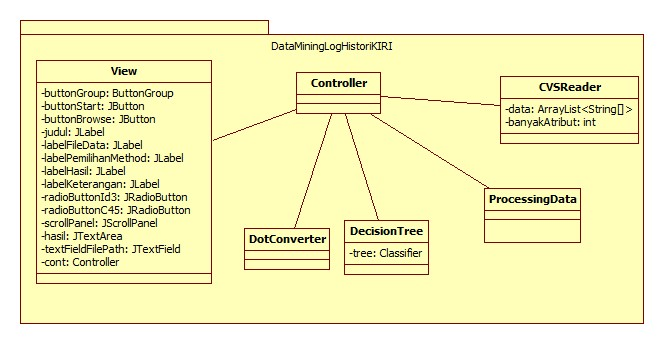
\includegraphics[scale=0.7]{Gambar/classdiagram.jpg}
\caption[Diagram \textsl{Class} Perangkat Lunak \textsl{Data Mining Log} Histori KIRI]{Diagram \textsl{Class} Perangkat Lunak \textsl{Data Mining Log} Histori KIRI} 
\label{fig:classDiagram}
\end{figure}

Berikut deskripsi kelas diagram \textsl{class}:
\begin{itemize}
	\item View, merupakan kelas untuk mengatur desain antar muka.
	\item Controller, merupakan kelas untuk mengatur view dan modul ketika program dijalankan.
	\item CSVReader, merupakan kelas yang memiliki method untuk membaca file dengan format CSV.
	\item ProcessingData, merupakan kelas yang memiliki method untuk melakukan \textsl{preprocessing data}.
	\item DecissionTree, merupakan kelas yang memiliki method untuk membuat \textsl{decision tree} dan menghitung \textsl{confident} dari pohon yang sudah dihasilkan.
	\item DotConverter, merupakan kelas yang memiliki method untuk mengubah \textsl{string} yang merupakan hasil dari kelas DecissionTree (yaitu, \textsl{decision tree} dalam bentuk string) menjadi bahasa DOT yang siap dijadikan \textsl{input} untuk graphviz.
\end{itemize}
	
















}{}
\ifdefstring{\vbabd}{1}{\chapter{Perancangan Perangkat Lunak}

Bab ini berisi tentang penjelasan perancangan perangkat lunak untuk melakukan proses \textsl{data mining} sesuai analisa yang sudah dibahas pada bab 3.

\section{Perancangan Perangkat Lunak}

\subsection{Perancangan Kelas}
Agar perangkat lunak dapat menjalankan fungsi yang sudah dibahas pada pemodelan fungsi di bab 3, maka pada subbab ini akan dibahas rancangan kelas dan \textsl{method} yang akan dibuat.

\begin{itemize}
	\item Kelas Controller, merupakan kelas untuk mengatur view dan modul ketika program dijalankan.
	\begin{itemize}
		\item Method
		\begin{itemize}
			\item public controller(), merupakan konstruktor dari kelas controller.
			\item public void startMining(String inputFilePath, String miningAlgo, JLabel label, JTextArea textArea), merupakan method untuk menjalankan modul-modul yang melakukan \textsl{data mining} dan membuat \textsl{decision tree} dari data yang menjadi masukan program.
			\item public static void main(String[] args), merupakan method main untuk menjalankan program.		
		\end{itemize}	
	\end{itemize}
	
	
	\item Kelas View, merupakan kelas untuk mengatur desain antar muka.
	\begin{itemize}
		\item Atribut
		\begin{itemize}
			\item ButtonGroup buttonGroup, digunakan untuk mengelompokkan jRadioButton.
			\item JButton buttonStart, merupakan sebuah tombol yang dapat memanggil method buttonStartActionPerformed() bila diklik.
			\item JButton buttonBrowse, merupakan sebuah tombol yang dapat memanggil method buttonBrowseActionPerformed() bila diklik.
			\item JLabel judul, merupakan sebuah label yang berisi judul dari aplikasi ini.
			\item JLabel labelFileData, merupakan label untuk menunjukkan bagian pemilihan file data \textsl{path}.
			\item JLabel labelPemilihanMethod, merupakan label untuk menunjukkan bagian pemilihan method.
			\item JLabel labelHasil, merupakan label untuk menunjukkan bagian hasil program.
			\item JLabel labelKeterangan, merupakan label untuk menunjukkan keterangan dari program.
			\item JRadioButton radioButtonId3, merupakan \textsl{radio button} yang menunjukkan bahwa user memilih metode ID3 atau tidak.
			\item JRadiioButton radioButtonC4.5, merupakan \textsl{radio button} yang menunjukkan bahwa user memilih metode C4.5 atau tidak.
			\item JScrollPanel scrollPanel, merupakan variabel yang digunakan untuk mengaktifkan fungsi scroll pada JTextArea hasil.
			\item JTextArea hasil, merupakan sebuah JTextArea yang digunakan untuk menunjukkan hasil \textsl{data mining} dari program.
			\item JTextField textFieldFilePath, digunakan untuk melakukan \textsl{input path file }baik dilakukan secara manual atau melalui tombol \textsl{browse}.
			\item Controller cont, digunakan untuk memanggil \textsl{method} startMining ketika tombol buttonStart diklik.
		\end{itemize}
		\item Method
		\begin{itemize}
			\item public void buttonBrowseActionPerformed(java.awt.event.ActionEvent evt), digunakan untuk membuat jFileChooser yang berfungsi untuk memilih file dan mendapatkan \textsl{file path} dari file yang dipilih dan memasukkan \textsl{string }tersebut ke textFieldFilePath.
			\item public void buttonStartActionPerformed(java.awt.event.ActionEvent evt), digunakan untuk mengambil String dari textFieldFilePath serta method yang dipilih pada jRadioButton (Id3 atau C4.5) kemudian memanggil method startMining dengan masukan kedua string tersebut, label dan textArea.
		\end{itemize}
	\end{itemize}

	\item Kelas CSVReader, merupakan kelas yang memiliki method untuk membaca file dengan format CSV.
	\begin{itemize}
		\item Atribut
		\begin{itemize}
			\item ArrayList<String[]> data, digunakan untuk menyimpan isi dari file CSV yang sudah dibaca.
			\item int banyakAtribut, digunakan untuk menyimpan banyak atribut yang akan dibaca oleh CSV.
		\end{itemize}
		\item Method
		\begin{itemize}
			\item public CSVReader(), merupakan konstruktor dari kelas CSVReader.
			\item public void setEmpty, merupakan method untuk menghapus isi variabel data.
			\item public ArrayList readCSV(String file), digunakan untuk membaca file CSV.
			\item public ArrayList getData(), digunakan untuk mendapatkan variabel data.
			\item public void setData(ArrayList data), digunakan untuk mengganti nilai variabel data sesuai dengan parameter.
			\item public int getBanyakAtribut(), digunakan untuk mendapatkan nilai variabel banyakAtribut.
			\item public void setBanyakAtribut(int banyakAtribut), digunakan untuk menggati nilai variabel banyakAtribut sesuai dengan parameter.
		\end{itemize}
	\end{itemize}

	\item Kelas ProcessingData, merupakan kelas yang memiliki method untuk melakukan \textsl{preprocessing data}.
	\begin{itemize}
		\item Method
		\begin{itemize}
			\item public ProcessingData(), merupakan konstruktor dari kelas ProcessingData.
			\item public void processSorting(ArrayList array, ArrayList data, String action), digunakan untuk memilah arraylist sehingga arraylist tersebut hanya berisi \textsl{action} yang diinginkan saja (pada penelitian ini, \textsl{action} yang diharapkan adalah FINDROUTE). Hasil pilah akan disimpan pada varibel array dari parameter method sehingga tidak diperlukan return value.
			\item public ArrayList preprocessingData(ArrayList<String[]> data), Digunakan untuk melakukan tahap \textsl{preprocessing data} seperti yang sudah dijelaskan pada pemodelan data di bab 3. Tujuan dari fungsi ini adalah mendapatkan nilai waktu yang sudah diubah menjadi GMT+7 dan sudah dikelompokkan menjadi jam, hari, bulan, dan tahun serta mengetahui klasifikasi kelas dari untuk setiap \textsl{record} dengan menghitung jarak dari titik keberangkatan terhadap titik pusat Bandung dan titik tujuan terhadap titik pusat Bandung.
			\item public int KlasifikasiKelas(double jarakKeberangkatan, double jarakTujuan), Digunakan untuk menentukan kelas dari hasil jarak titik keberangkatan dengan titik pusat Bandung dan titik tujuan dengan titik pusat Bandung. 
		\end{itemize}
	\end{itemize}

	\item Kelas DecisionTree, merupakan kelas yang memiliki method untuk membuat \textsl{decision tree} dan menghitung akurasi dari pohon yang sudah dihasilkan.
	\begin{itemize}
		\item Atribut
		\begin{itemize}
			\item Classifier tree, digunakan untuk menyimpan \textsl{decision tree} yang sudah dihasilkan.
		\end{itemize}
		\item Method
		\begin{itemize}
			\item public DecisionTree(), merupakan konstruktor untuk kelas DecisionTree.
			\item public double calculatePrecision(Instances data), digunakan untuk mendapatkan nilai akurasi dari \textsl{decision tree} yang dihasilkan.
			\item public String id3(Instances data), digunakan untuk membuat \textsl{decision tree} dengan menggunakan metode ID3 dari API Weka.
			\item public String j48(Instances data), digunakan untuk membuat \textsl{decision tree} dengan menggunakan metode C4.5 dari API Weka.
		\end{itemize}
	\end{itemize}

	\item Kelas Dot Converter, merupakan kelas yang memiliki method untuk mengubah \textsl{string} yang merupakan hasil dari kelas DecissionTree (yaitu, \textsl{decision tree} dalam bentuk string) menjadi bahasa dot yang siap dijadikan masukan untuk graphviz.
	\begin{itemize}
		\item Method
		\begin{itemize}
			\item public String convert(String data, String miningAlgo, String nodeName), Digunakan untuk mengubah nilai string yang sudah diperoleh dari kelas DecisionTree menjadi bahasa DOT untuk membuat visualisasi dengan menggunakan graphviz.
		\end{itemize}
	\end{itemize}
\end{itemize}
	
	Pada kelas ProcessingData, nilai data waktu perlu diganti menjadi GMT+7 dan perlu menghitung jarak antar dua titik. Maka dari itu, akan dibuat dua kelas tambahan untuk melakukan kedua hal tersebut, yaitu TimezoneConverter dan DistanceHaversine.
	
\begin{itemize}
	\item Kelas TimezoneConverter, merupakan kelas yang memiliki \textsl{method} untuk mengubah waktu dari UTC menjadi GMT+7
	\begin{itemize}
		\item Method
		\begin{itemize}
			\item public static String convertToGMT7(String date), digunakan untuk mengubah waktu dari UTC menjadi GMT+7.
		\end{itemize}
	\end{itemize}

	\item Kelas DistanceHaversine, kelas yang memiliki \textsl{method} untuk menghitung jarak dua titik di bumi.
	\begin{itemize}
		\item Atribut
		\begin{itemize}
			\item double r, digunakan untuk menyimpan nilai radius dari bumi.
		\end{itemize}
		\item Method
		\begin{itemize}
			\item public double calculateDistance(double latitude1, double longitude1, double latitude2, double longitude2), Digunakan untuk menghitung jarak dari dua titik (latitude dan longitude).
		\end{itemize}
	\end{itemize}
\end{itemize}

	Setelah melakukan penelitian tentang API Weka, diperoleh bahwa input untuk membuat \textsl{decision tree} merupakan kelas Instances dari API Weka. Selain itu, diperlukan juga pengecekkan untuk hasil dari kelas tersebut, apakah sudah sesuai dengan aplikasi Weka atau belum (karena menggunakan API Weka, seharusnya \textsl{decision tree} yang dihasilkan sama). Oleh karena itu, akan ditambahkan kelas ArffIO yang berfungsi untuk menulis dan membaca data dengan format arff, sehingga ketika program melakukan \textsl{data mining}, program akan menghasilkan file dengan format .arff yang dapat dibaca oleh aplikasi Weka untuk melakukan pengetesan. Karena kita sudah memiliki file .arff tersebut, ada baiknya jika menggunakan fungsi membaca arff dari API Weka yang menghasilkan \textsl{return value} berupa kelas Instances yang dapat digunakan untuk membuat \textsl{decision tree}.

\begin{itemize}
	\item Kelas ArffIO, merupakan kelas yang berfungsi untuk melakukan penyimpanan dan membaca data dengan format arff.
	\begin{itemize}
		\item Method
		\begin{itemize}
			\item public ArffIO, merupakan konstruktor dari kelas ArffIO.
			\item public void writeArffIO(String name, ArrayList<int[]> data), digunakan untuk menulis file .arff sesuai data pada parameter.
			\item public Instances arffRead(String name), digunakan untuk membaca file .arff dengan menggunakan \textsl{method} dari API Weka.
		\end{itemize}
	\end{itemize}
\end{itemize}

Ketika mulai merancang \textsl{method} convert yang berada di kelas DotConverter, akan lebih mudah jika dirancang menjadi rekursif. Karena data yang diolah pada \textsl{method}
tersebut cukup banyak dan diperlukan nama yang berbeda pada setiap node yang akan ditulis pada DOT, maka perlu ditambah kelas yang berfungsi untuk struktur data pada kelas tersebut, yaitu SDForConvertTree.

\begin{itemize}
	\item kelas SDForConvertTree, kelas yang berfungsi untuk menyimpan data yang dibutuhkan untuk mengubah String hasil dari kelas DecisionTree menjadi bahasa DOT.
	\begin{itemize}
		\item Atribut
		\begin{itemize}
			\item String[] data, digunakan untuk menyimpan nama-nama atribut yang akan diubah ke dalam bahasa DOT.
			\item int[] count, digunakan untuk menghitung penggunaan nama setiap atribut sehingga dapat menghasilkan nama node yang berbeda untuk setiap atribut.
		\end{itemize}
		\item Method
		\begin{itemize}
			\item public SDForConvertTree(String[] data), merupakan konstruktor untuk kelas ini dan akan melakukan inisialisasi data pada atribut dengan nilai data pada parameter serta melakukan inisialisasi nilai variabel count dengan 0.
			\item public void setData(String data, index int), digunakan untuk mengubah nilai data pada index tertentu.
			\item public String[] getData(), digunakan untuk mendapatkan nilai atribut data.
			\item public String getData(int index), digunakan untuk mendapatkan nilai data pada index tertentu.
			\item public void setCount(int count, int index), digunakan untuk mengubah nilai count pada index tertentu.
			\item public int getCount(int index), digunakan untuk mendapatkan nilai count pada index tertentu.
			\item public boolean hasNext(), digunakan untuk mengecek apakah isi dari varibel data masih ada atau tidak.
			\item public void buangArrayPertama(), digunakan untuk membuang nilai array yang pertama (index ke-0).
			\item public String getDataNumber(String atribut), digunakan untuk mendapatkan angka pada nama atribut tertentu untuk membuat nama node pada kelas DotConverter agar semua nama node berbeda.
		\end{itemize}
	\end{itemize}
\end{itemize}

Setelah melakukan \textsl{convert} dari \textsl{string} hasil dari \textsl{method} pembuatan \textsl{decision tree} dari API Weka ke bahasa Dot, maka diperlukan pemanggilan fungsi dot yang terdapat pada graphviz. Cara memanggilan fungsi tersebut yaitu dengan menggunakan \textsl{command prompt}. Maka dari itu, akan diperlukan kelas yang memiliki \textsl{method} untuk memanggil \textsl{command prompt} dan menjalankan fungsi dot tersebut, yaitu kelas CMD.


\begin{itemize}
	\item kelas CMD, merupakan kelas yang digunakan untuk memanggil \textsl{command prompt}.
	\begin{itemize}
		\item Method
		\begin{itemize}
			\item public static void makeJpgUsingDotCommand(), digunakan untuk memanggil \textsl{command prompt} dan menjalankan fungsi dot dan menghasil gambar visualisasi grafik sesuai dengan file yang menjadi masukan fungsi tersebut.
		\end{itemize}
	\end{itemize}
\end{itemize}

Karena cara yang untuk memanggil fungsi dot adalah \textsl{command prompt}, maka hasil dari \textsl{method} convert harus disimpan dalam bentuk file text agar dapat dibaca oleh \textsl{command prompt}.

Dari perancangan kelas dan \textsl{method} yang sudah dilakukan, maka akan diperoleh diagram kelas seperti pada \ref{fig:classDiagram2}

\begin{figure}[H]
\includegraphics[scale=0.5, angle =90]{Gambar/classdiagram2.jpg}
\caption[Diagram \textsl{Class} Perangkat Lunak \textsl{Data Mining Log} Histori KIRI]{Diagram \textsl{Class} Perangkat Lunak \textsl{Data Mining Log} Histori KIRI} 
\label{fig:classDiagram2}
\end{figure}

\subsection{Sequence Diagram}

Pada subbab ini, akan dijelaskan alur program dengan menggunakan \textsl{sequence diagram} pada \ref{fig:sequenceDiagram}.

Pertama, program akan menampilkan desain antar muka yang dihasilkan oleh kelas View. Kemudian user akan menulis \textsl{file path} atau memilih (dengan menggunakan tombol \textsl{browse}) \textsl{input} file pada JTextField serta memilih metode pembuatan \textsl{decision tree} (tahap  pertama). Setelah memilih file dan metode, user akan menekan tombol start, dan kelas View akan memanggil \textsl{method} startMining dari kelas controller (tahap 3-4).

Kelas Controller akan mengakses file sesuai dengan masukan \textsl{file path} dengan memanggil \textsl{method} readCSV dari kelas CSVReader dan mendapat nilai kembalian berupa arraylist (tahap 5-6). Setelah mendapatkan data dari file CSV yang dipilih, data tersebut akan dipilah dan menggambil \textsl{record} dengan \textsl{action} FINDROUTE dengan cara memanggil \textsl{method} processSorting pada kelas ProcessingData dan mengembalikan ArrayList dengan data yang sudah dipilah (tahap 7-8). Kemudian data tersebut akan dilakukan \textsl{preprocessing data} dengan cara memanggil \textsl{method} preprocessingData dari kelas ProcessingData(tahap 9).

Ketika \textsl{method} preprocessingData dijalankan, perlu mengubah nilai waktu dari UTC menjadi GMT+7 dengan cara memanggil \textsl{method} convertGMT7 dari kelas TimezoneConverter dan mengembalikan nilai bertipe Date (tahap 10-11). Setelah nilai waktu diubah, diperlukan perhitungan jarak antara dua titik dengan cara memanggil \textsl{method} calculateDistance  dari kelas DistanceHaversine dan mengembalikan nilai double yang berisi jarak dari kedua titik(tahap 12-13). Kemudian diperlukan klasifikasi kelas dari jarak yang sudah dihasilkan dengan cara memanggil \textsl{method} klasifikasiKelas dari kelas ProcessingData (tahap 14-15). Kemudian semua data yang sudah diproses akan dikembalikan dalam bentuk ArrayList(tahap 16).

Setelah didapat data yang sudah dilakukan \textsl{preprocessing data}, data tersebut akan disimpan dengan format arff dengan cara memanggi \textsl{method} writeArff pada kelas ArffIO(tahap 17). Setelah disimpan, diperlukan mengambil data dari file arff yang sudah disimpan untuk mendapatkan data dengan tipe Instance dengan cara memanggil \textsl{method}readArff(tahap 18-19).

Kemudian program akan membuat \textsl{decision tree} dengan cara memanggil \textsl{method} id3 atau j48 pada kelas DecisionTree dan mengembalikan \textsl{decision tree} dalam bentuk \textsl{String}(tahap 20-21). Setelah \textsl{decision tree} dibuat, perlu dicari nilai akurasi yang diperoleh dari \textsl{decision tree} tersebut dengan cara memanggil \textsl{method} calculatePrecision dan nilai akurasi yang dihasilkan dikembalikan dalam bentuk double(tahap 22-23).

Tahap selanjutnya adalah mengubah nilai String yang diperoleh dari \textsl{method} id3 atau j48 menjadi bahasa DOT dengan cara memanggil \textsl{method} convert pada kelas DotConverter dan akan mengembalikan nilai String(tahap 24-25). Setelah diperoleh hasil dari \textsl{method} convert, maka diperlukan \textsl{command prompt} untuk menghasilkan gambar grafik untuk melakukan visualisasi \textsl{decision tree} yang sudah dihasilkan(tahap 26-27).

Setelah gambar \textsl{decision tree} dihasilkan, maka \textsl{method} startMining akan membuat JFrame yang baru untuk memperlihatkan hasil gambar \textsl{decision tree} yang sudah diperoleh serta mengembalikan nilai String \textsl{decision tree} kepada kelas View yang akan ditampilkan di JTextArea(tahap 28-29).


\begin{figure}[H]
\includegraphics[scale=0.42, angle =90]{Gambar/sequenceDiagram.jpg}
\caption[Diagram \textsl{Class} Perangkat Lunak \textsl{Data Mining Log} Histori KIRI]{Diagram \textsl{Class} Perangkat Lunak \textsl{Data Mining Log} Histori KIRI} 
\label{fig:sequenceDiagram}
\end{figure}

\subsection{Perancangan Desain Antar Muka}

Pada subbab ini, akan diperlihatkan rancangan desain antar muka yang akan digunakan untuk program ini.

Aplikasi ini memiliki dua form untuk melakukan \textsl{data mining} dan membuat \textsl{decision tree}. Pada form pertama(dapat dilihat di \ref{fig:MU1}) disediakan JTextbox dan JButton yang digunakan untuk memilih file, JRadioButton yang digunakan untuk memilih metode pembuatan \textsl{decision tree}, JTextArea yang digunakan untuk memperlihatkan hasil \textsl{decision tree} yang diperoleh dalam bentuk String, serta JTextButton yang kedua (dengan label Start) yang digunakan untuk memulai proses \textsl{data mining}. Sedangkan form kedua, berisi gambar visualisasi \textsl{decision tree} yang sudah dihasilkan(dapat dilihat di \ref{fig:MU2}).
\begin{figure}[H]
\centering
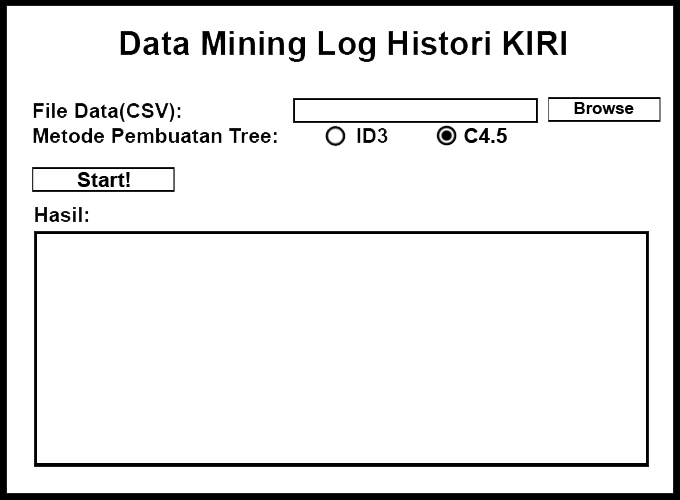
\includegraphics[scale=1.2]{Gambar/mockUp1.jpg}
\caption[Mock Up Form Pertama]{Mock Up Form Pertama} 
\label{fig:MU1}
\end{figure}

\begin{figure}[H]
\centering
\includegraphics[scale=1.2]{Gambar/mockUp2.jpg}
\caption[Mock Up Form Kedua]{Mock Up Form Kedua} 
\label{fig:MU2}
\end{figure}}{}
\ifdefstring{\vbabe}{1}{\chapter{Implementasi Program dan Pengujian}

Bab ini menjelaskan tentang lingkupan pembangunan, implementasi rancangan antarmuka, serta pengujian secara fungsional dan experimental pada aplikasi \textsl{data mining}.

\section{Lingkungan Pembangunan}
Lingkungan perangkat lunak dan perangkat keras yang digunakan untuk membangun dan menguji aplikasi \textsl{data mining} ini adalah:

\begin{enumerate}
	\item CPU
	\begin{itemize}
		\item Prosesor: Intel(R) Core(TM) i7, 1.60 GHz
		\item RAM: 6 GB
		\item VGA: NVDIA GeForce GT 330M
		\item Hardisk: 300 GB
	\end{itemize}
	\item Sistem operasi: Windows 7 Professional
	\item Platform: NetBeans: IDE 8.0
\end{enumerate}

\section{Hasil Tampilan Antarmuka}
Pada aplikasi \textsl{data mining} ini, terdapat dua form. Form pertama berfungsi untuk memilih file CSV yang dilakukan \textsl{data mining}, memilih metode pembuatan \textsl{decision tree}, serta menunjukkan hasil \textsl{decision tree} yang dihasilkan dalam bentuk String. Sedangkan untuk form kedua, berfungsi untuk memvisualisasikan \textsl{decision tree} yang sudah diperoleh dalam bentuk gambar.

TextField yang pertama berfungsi untuk mengisi alamat file CSV yang dilakukan \textsl{data mining}. RadioButton berfungsi untuk memilih metode manakah yang digunakan untuk membuat \textsl{decision tree}. TextArea digunakan untuk memperlihatkan hasil \textsl{decision tree} dalam bentuk String. Tampilan awal aplikasi dapat dilihat di \ref{fig:GUI1}.

\begin{figure}[H]
\centering
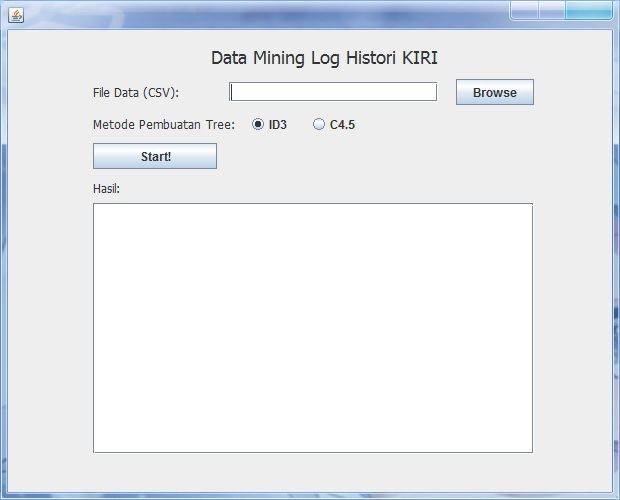
\includegraphics[scale=0.7]{Gambar/GUI1.jpg}
\caption[Tampilan Form Awal Aplikasi \textsl{Data Mining}]{Tampilan Form Awal Aplikasi \textsl{Data Mining}} 
\label{fig:GUI1}
\end{figure}

Terdapat dua cara untuk mengisi TextField, yaitu ditulis secara manual alamat file CSV atau dengan cara mengklik tombol button browse dan memilih file CSV pada FileSelector. Tampilan memilih file CSV dapat dilihat pada gambar \ref{fig:GUI2} dan tampilan setelah memilih file CSV dapat dilihat pada gambar \ref{fig:GUI3}.

\begin{figure}[H]
\centering
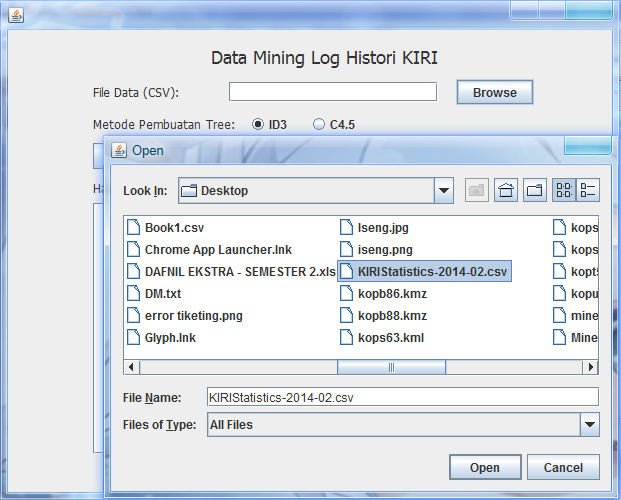
\includegraphics[scale=0.7]{Gambar/GUI2.jpg}
\caption[Tampilan FileSelector untuk Memilih File CSV]{Tampilan FileSelector untuk Memilih File CSV} 
\label{fig:GUI2}
\end{figure}

\begin{figure}[H]
\centering
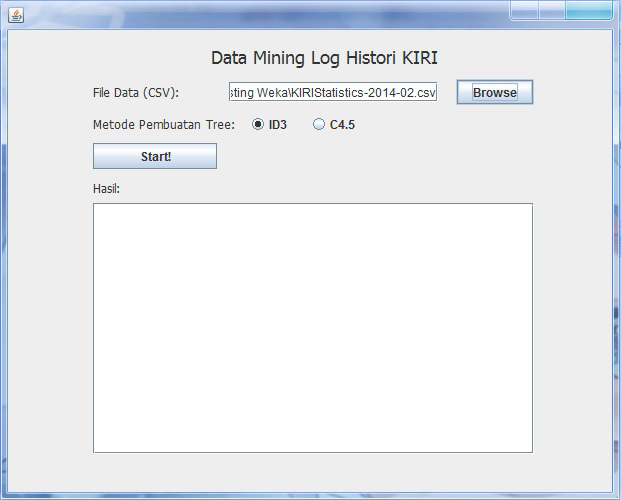
\includegraphics[scale=0.7]{Gambar/GUI3.jpg}
\caption[Tampilan Form setelah Memilih File CSV]{Tampilan Form setelah Memilih File CSV} 
\label{fig:GUI3}
\end{figure}

Setelah alamat file CSV diisi, hal selanjutnya yang dilakukan adalah memilih metode pembuatan \textsl{decision tree} pada RadioButton. RadioButton memilih metode ID3 jika \textsl{setting} ini tidak diubah. Tampilan tersebut dapat dilihat di gambar \ref{fig:GUI3and4}.

\begin{figure}[H]
\centering
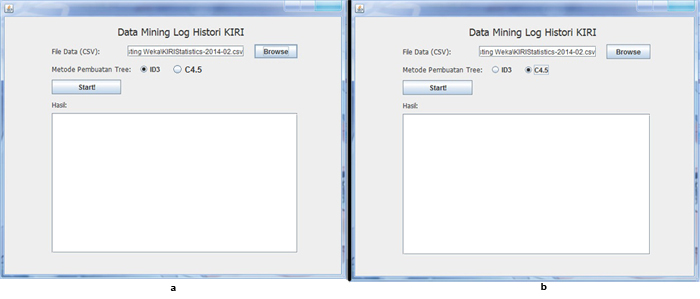
\includegraphics[scale=0.5]{Gambar/GUI3and4.jpg}
\caption[Tampilan Form Pemilihan Metode Pembuatan \textsl{Decision Tree}]{Tampilan Form Pemilihan Metode Pembuatan \textsl{Decision Tree}. Gambar a merupakan kondisi tampilan ketika metode ID3 dipilih sedangkan gambar b merupakan kondisi tampilan ketika metode C4.5 dipilih.} 
\label{fig:GUI3and4}
\end{figure}

Kemudian, tombol start diklik lalu program melakukan proses \textsl{data mining}. Setelah selesai, program menunjukkan hasil \textsl{data mining} dalam bentuk String pada TextArea dan dalam bentuk gambar pada form kedua. Tampilan akhir dari aplikasi serta form kedua dapat dilihat di gambar \ref{fig:GUI5}.

\begin{figure}[H]
\centering
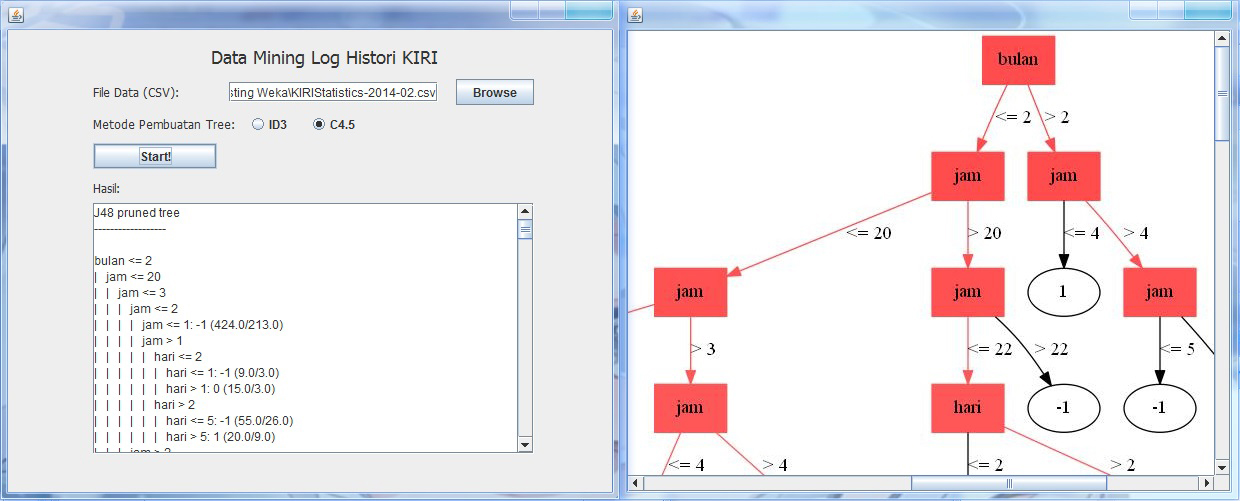
\includegraphics[scale=0.4]{Gambar/GUI5.jpg}
\caption[Tampilan Form Menampilkan Hasil \textsl{Data Mining}]{Tampilan Form Menampilkan Hasil \textsl{Data Mining}} 
\label{fig:GUI5}
\end{figure}

\section{Pengujian Aplikasi \textsl{Data Mining}}

\subsection{Pengujian Fungsional}

\subsubsection{Rancangan Pengujian}

Dalam pengujian aplikasi \textsl{data mining} ini, digunakan teknik pengujian \textsl{black box}. Pengujian yang dilakukan:
\begin{enumerate}
	\item Pengujian \textsl{method} utama untuk mencapai tujuan dari aplikasi \textsl{data mining} ini. Terdapat beberapa \textsl{method} yang perlu diuji, yaitu
	\begin{enumerate}
		\item Membaca file CSV
		\item Melakukan \textsl{preprocessing data}
		\item Membuat \textsl{decision tree}
		\item Mengubah \textsl{decision tree} dalam bentuk String menjadi bahasa DOT
	\end{enumerate}
	\item Kebenaran perangkat lunak hanya dilihat pada hasil keluaran program atau kondisi masukan yang diberikan tanpa melihat bagaimana proses untuk mendapatkan keluaran tersebut.
	\item Dari keluaran yang dihasilkan, kemampuan program untuk memenuhi kebutuhan pemakai dapat diukur dan dapat diketahui kesalahan jika ada.
\end{enumerate}


\subsubsection{Hasil Pengujian}

Dibuat sebuah \textsl{test case} yang berisi 20 data \textsl{log} histori KIRI dengan data pada tabel \ref{table:dataTestCase}

\begin{table}[H]
\rotatebox{90}{
\begin{tabular}{|l|l|l|l|l|}
\hline
\textbf{logId} & \textbf{APIKey}  & \textbf{Timestamp (UTC)} & \textbf{Action} & \textbf{AdditionalData}                                        \\ \hline
114055         & E5D9904F0A8B4F99 & 2/1/2014 2:34            & FINDROUTE       & -6.88968,107.59632/-6.88461,107.61361/3                        \\ \hline
114056         & E5D9904F0A8B4F99 & 2/1/2014 2:34            & FINDROUTE       & -6.88968,107.59632/-6.88461,107.61361/3                        \\ \hline
114057         & E5D9904F0A8B4F99 & 2/1/2014 2:34            & FINDROUTE       & -6.88968,107.59632/-6.88461,107.61361/3                        \\ \hline
114058         & A44EB361A179A49E & 2/1/2014 2:35            & FINDROUTE       & -6.9112484,107.6275648/-6.875449306549391,107.60455314069986/1 \\ \hline
114059         & E5D9904F0A8B4F99 & 2/1/2014 2:37            & PAGELOAD        & /5.10.83.99/                                                   \\ \hline
114060         & A44EB361A179A49E & 2/1/2014 2:38            & SEARCHPLACE     & cimol\%2C+/10                                                  \\ \hline
114061         & A44EB361A179A49E & 2/1/2014 2:38            & FINDROUTE       & -6.8779112,107.612129/-6.92663,107.63644/1                     \\ \hline
114062         & A44EB361A179A49E & 2/1/2014 2:38            & SEARCHPLACE     & gedebage\%2C+/10                                               \\ \hline
114063         & A44EB361A179A49E & 2/1/2014 2:38            & SEARCHPLACE     & gedebage\%2C+cimol/10                                          \\ \hline
114064         & A44EB361A179A49E & 2/1/2014 2:39            & FINDROUTE       & -7.3275023,108.3614085/-6.93269,107.69734/1                    \\ \hline
114065         & A44EB361A179A49E & 2/1/2014 2:39            & WIDGETLOAD      & /66.249.77.219/                                                \\ \hline
114066         & A44EB361A179A49E & 2/1/2014 2:39            & FINDROUTE       & -6.863680050774415,107.5951399281621/-6.93269,107.69734/1      \\ \hline
114067         & A44EB361A179A49E & 2/1/2014 2:43            & FINDROUTE       & -6.9423325,107.7486968/-6.90112,107.60787/1                    \\ \hline
114068         & A44EB361A179A49E & 2/1/2014 2:43            & FINDROUTE       & -6.9423325,107.7486968/-6.88623,107.60821/1                    \\ \hline
114069         & A44EB361A179A49E & 2/1/2014 2:44            & FINDROUTE       & -6.9423062,107.7490084/-6.88623,107.60821/1                    \\ \hline
114070         & A44EB361A179A49E & 2/1/2014 2:45            & FINDROUTE       & -6.9072888,107.6143937/-6.90855,107.61082/1                    \\ \hline
114071         & A44EB361A179A49E & 2/1/2014 2:46            & FINDROUTE       & -6.9286306,107.6227444/-6.91708,107.60880/1                    \\ \hline
114072         & A44EB361A179A49E & 2/1/2014 2:46            & FINDROUTE       & -6.908639785445589,107.61091567575932/-6.90855,107.61082/1     \\ \hline
114073         & A44EB361A179A49E & 2/1/2014 2:47            & SEARCHPLACE     & hotel+harapan+i/10                                             \\ \hline
114074         & A44EB361A179A49E & 2/1/2014 2:47            & SEARCHPLACE     & hotel+harapan+ind/10                                           \\ \hline
\end{tabular}}
\caption{Data untuk \textsl{Test Case} Aplikasi \textsl{Data Mining}}
\label{table:dataTestCase}
\end{table}

Berikut hasil pengujian yang dilakukan dengan menggunakan data tersebut:
\begin{enumerate}
	\item Pengujian pertama: Membaca file CSV, data diambil oleh program dan dipilah, hanya record dengan \textsl{action} FINDROUTE yang diambil sedangkan yang lain dibuang. Berikut hasil dengan contoh data diatas dengan menggunakan sistem \textsl{debug} untuk melihat data yang diambil dari CSV pada gambar \ref{fig:Pengujian1} dan \ref{fig:Pengujian12}
	
	\begin{figure}[H]
	\centering
	\includegraphics[scale=0.4]{Gambar/pengujian1.jpg}
	\caption[Pengujian Mengambil Data CSV]{Pengujian Mengambil Data CSV} 
	\label{fig:Pengujian1}
	\end{figure}

	\begin{figure}[H]
	\centering
	\includegraphics[scale=0.4]{Gambar/pengujian12.jpg}
	\caption[Pengujian \textsl{Data Selection} untuk Mengambil Data dengan \textsl{Action} FINDROUTE]{Pengujian \textsl{Data Selection} untuk Mengambil Data dengan \textsl{Action} FINDROUTE} 
	\label{fig:Pengujian12}
	\end{figure}

	Gambar pertama memperlihatkan bahwa data pertama yang diperoleh 21 array String dengan array pertama adalah atributnya sedangkan array selanjutnya adalah isi data yang diperoleh. Pada gambar kedua, terdapat 13 array String dimana semua array tersebut merupakan record dengan nilai \textsl{action} FINDROUTE saja. Dengan demikian, pengujian membaca CSV berhasil dilakukan.

	\item Pengujian kedua: Melakukan \textsl{preprocessing data}, data yang digunakan adalah 13 array String yang sudah diperoleh dari pengujian pertama. Pengujian dilakukan dengan cara mengecek data menggunakan weka untuk melihat data yang sudah dihasilkan. Hasil yang diperoleh dari pengujian dapat dilihat pada \ref{fig:Pengujian214} dan \ref{fig:Pengujian25} 
	
	\begin{figure}[ht]
	\centering
	\includegraphics[scale=0.35]{Gambar/pengujian214.jpg}
	\caption[Pengujian \textsl{Preprocessing Data}]{Pengujian \textsl{Preprocessing Data}. Gambar a menunjukkan nilai pada atribut bulan. Gambar b menunjukkan nilai pada atribut tahun. Gambar c menunjukkan nilai pada atribut hari. Gambar d menunjukkan nilai pada atribut jam.} 
	\label{fig:Pengujian214}
	\end{figure}
	
	\begin{figure}[ht]
	\centering
	\includegraphics[scale=0.4]{Gambar/pengujian25.jpg}
	\caption[Pengujian \textsl{Preprocessing Data} untuk Klasifikasi Data]{Pengujian \textsl{Preprocessing Data} untuk Klasifikasi Data} 
	\label{fig:Pengujian25}
	\end{figure}

	Terdapat dua tahap penting pada \textsl{prerpocessing data}, yaitu pengubahan waktu dari UTC menjadi GMT+7 dan klasifikasi area. Pada tahap pengubahan waktu dari UTC menjadi GMT+7, pada gambar \ref{fig:Pengujian214} d, atribut jam yang dimiliki menjadi bernilai sembilan karena pada testcase, nilai atribut jam adalah dua. Pada tahap klasifikasi area, dapat dilihat pada tabel \ref{table:PenentuanAreaDanKlasifikasi}
	
	\begin{table}[ht]
	\centering
	\begin{tabular}{|l|l|l|}
	\hline
	\multicolumn{1}{|c|}{\textbf{Region Keberangkatan}} & \multicolumn{1}{c|}{\textbf{Region Tujuan}} & \multicolumn{1}{c|}{\textbf{Hasil Klasifikasi}} \\ \hline
	3                                                   & 3                                           & 0                                               \\ \hline
	3                                                   & 3                                           & 0                                               \\ \hline
	3                                                   & 3                                           & 0                                               \\ \hline
	3                                                   & 4                                           & 1                                               \\ \hline
	4                                                   & 4                                           & 0                                               \\ \hline
	11                                                  & 10                                          & -1                                              \\ \hline
	5                                                   & 10                                          & 1                                               \\ \hline
	11                                                  & 1                                           & -1                                              \\ \hline
	11                                                  & 3                                           & -1                                              \\ \hline
	11                                                  & 3                                           & -1                                              \\ \hline
	1                                                   & 1                                           & 0                                               \\ \hline
	2                                                   & 0                                           & -1                                              \\ \hline
	1                                                   & 1                                           & 0                                               \\ \hline
	\end{tabular}
	\caption{Hasil Penentuan area dan Klasifikasi}
	\label{table:PenentuanAreaDanKlasifikasi}
	\end{table}
	
	Terdapat lima data dengan klasifikasi -1, enam data dengan klasifikasi 0, dan 2 data dengan klasifikasi 1. Dari kedua hasil tersebut, dapat disimpulkan bahwa tahap \textsl{preprocessing data} sudah berjalan dengan baik.
	
	\item Pengujian ketiga: Membuat \textsl{decision tree}, dilakukan perbandingan antara hasil dari program dengan hasil dari weka, dapat dilihat pada gambar \ref{fig:Pengujian31} dan 
	\ref{fig:Pengujian32}. Dari kedua gambar tersebut, dapat disimpulkan bahwa hasil \textsl{decision tree} yang dihasilkan sama dan benar.
	
	\begin{figure}[ht]
	\centering
	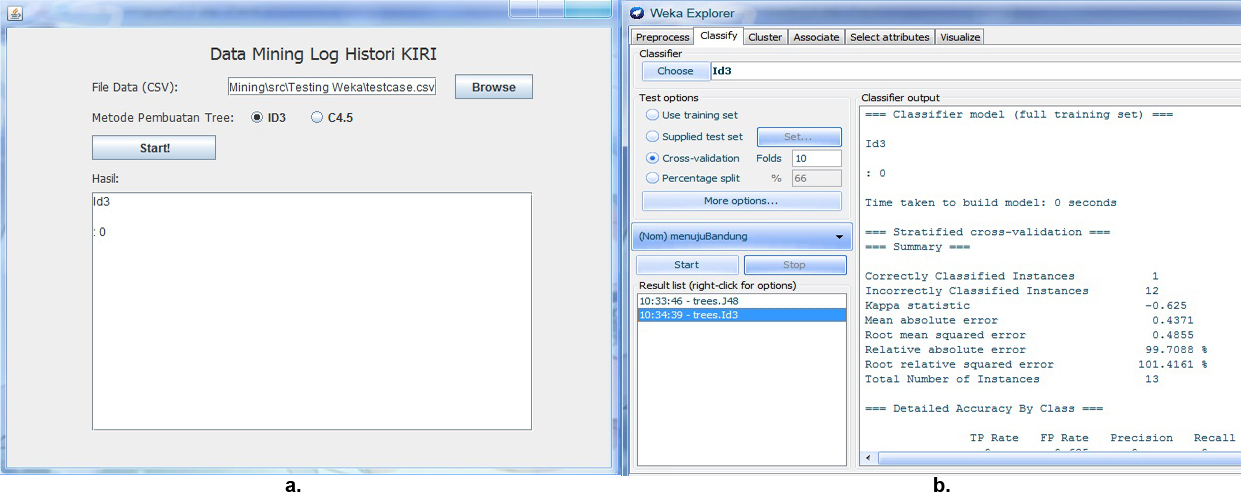
\includegraphics[scale=0.4]{Gambar/pengujian31.jpg}
	\caption[Pengujian Pembuatan \textsl{Decision Tree} ID3]{Pengujian Pembuatan \textsl{Decision Tree} ID3. Gambar a merupakan hasil dari aplikasi \textsl{data mining} sedangkan gambar b merupakan hasil dari weka.} 
	\label{fig:Pengujian31}
	\end{figure}

	\begin{figure}[ht]
	\centering
	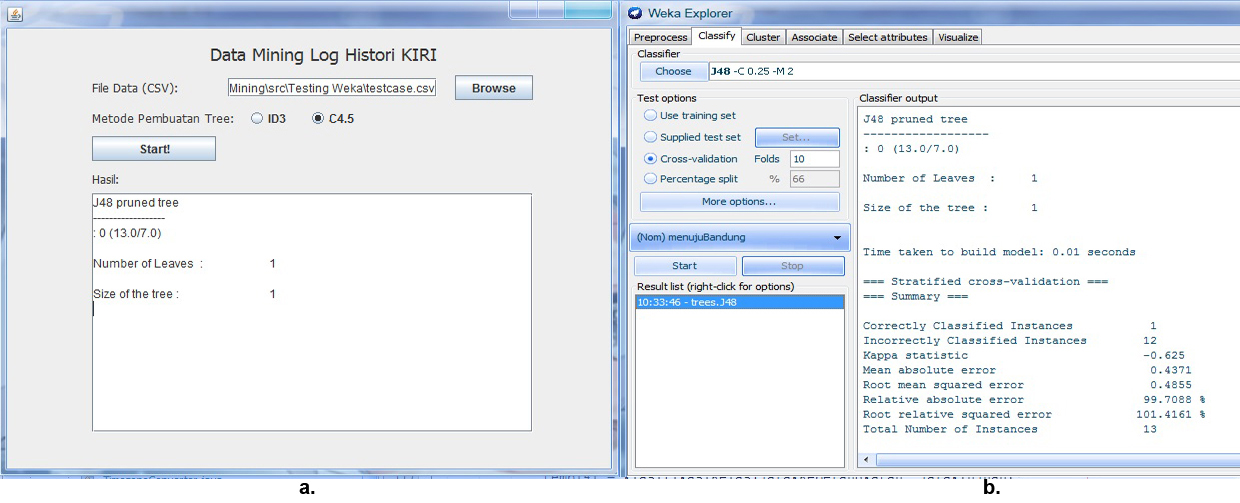
\includegraphics[scale=0.4]{Gambar/pengujian32.jpg}
	\caption[Pengujian Pembuatan \textsl{Decision Tree} C4.5]{Pengujian  Pembuatan \textsl{Decision Tree} C4.5. Gambar a merupakan hasil dari aplikasi \textsl{data mining} sedangkan gambar b merupakan hasil dari weka.} 
	\label{fig:Pengujian32}
	\end{figure}

	
	\item Pengujian keempat: Mengubah \textsl{decision tree} dalam bentuk String menjadi bahasa DOT, melakukan visualisasi \textsl{decision tree} dengan membuat graph dalam bahasa DOT, dapat dilihat pada gambar \ref{fig:Pengujian4}. Dari gambar tersebut, dapat disimpulkan bahwa pengubahan \textsl{decision tree} menjadi bahasa DOT telah berhasil.
	
	\begin{figure}[H]
	\centering
	\includegraphics[scale=0.4]{Gambar/pengujian4.jpg}
	\caption[Pengujian Hasil Visualisasi dengan Menggunakan Bahasa DOT]{Pengujian Hasil Visualisasi dengan Menggunakan Bahasa DOT.} 
	\label{fig:Pengujian4}
	\end{figure}
	

\end{enumerate}

\subsection{Pengujian Eksperimental}

Pada subbab ini, dilakukan pengujian pada data 1 bulan dari \textsl{log} histori KIRI bulan Febuari.

Ketika Pengujian dilakukan, ditemukan \textsl{bug} data yaitu terdapat nilai dari data \textsl{log} histori KIRI pada \textsl{action} FINDROUTE kolom additionalData dengan format String yang berbeda. Kesalahan format tersebut adalah nilai pembatas angka dibelakang koma yang seharusnya menggunakan titik menjadi koma, sehingga pemotongan nilai String menghasilkan data yang salah dan menyebabkan \textsl{error} berupa data tidak dapat diproses. Dari pengujian ini, maka diperlukan \textsl{data cleaning} pada tahap \textsl{preprocessing data} agar data dengan format yang salah dapat dibuang dan tidak menyebabkan \textsl{error}. Hasil error yang ditemukan dari \textsl{data cleaning} dapat dilihat pada gambar \ref{fig:percobaanError}.

\begin{figure}[H]
\centering
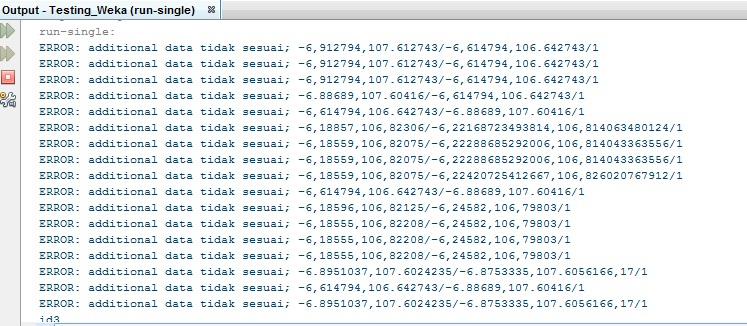
\includegraphics[scale=0.5]{Gambar/percobaanError.jpg}
\caption[Percobaan \textsl{Data Mining} untuk Melakukan Data Cleaning]{Percobaan \textsl{Data Mining} untuk Melakukan Data Cleaning.} 
\label{fig:percobaanError}
\end{figure}

Setelah melakukan \textsl{data cleaning}, program dapat berjalan dengan baik. Berikut hasil dari percobaan metode ID3 pada gambar \ref{fig:percobaan1} dan metode C4.5 pada gambar \ref{fig:percobaan2}.

\begin{figure}[H]
\centering
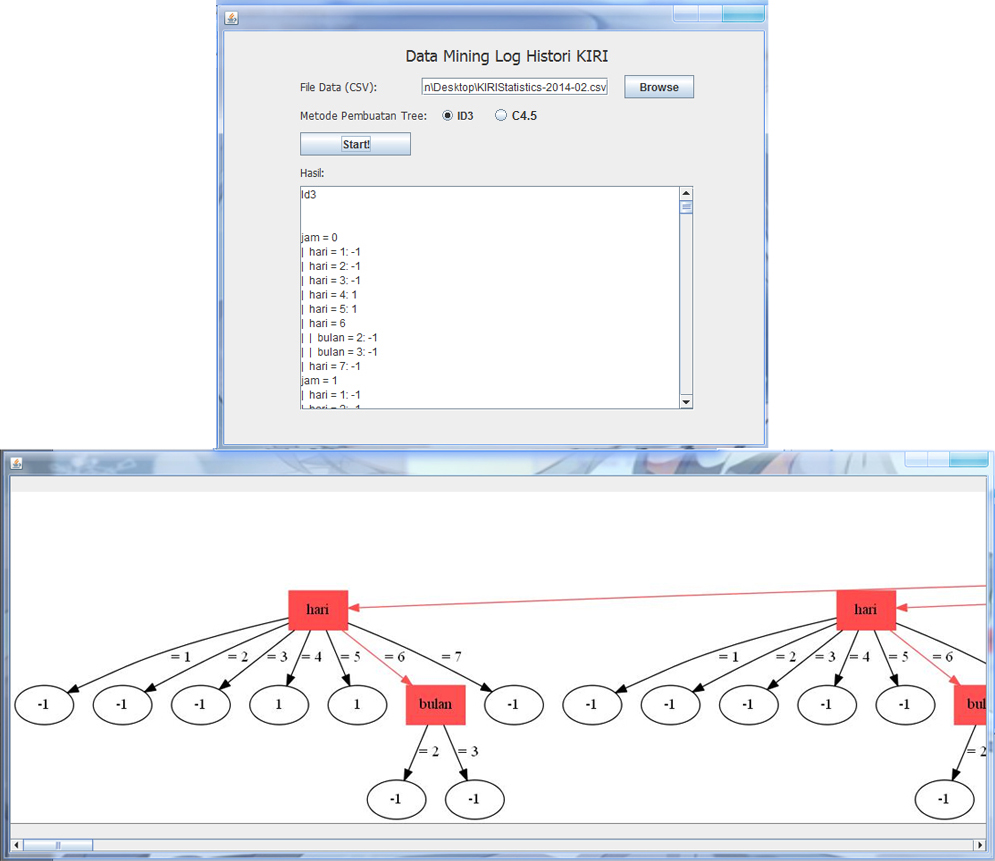
\includegraphics[scale=0.43]{Gambar/percobaan1.jpg}
\caption[Percobaan \textsl{Data Mining} dengan Menggunakan Metode ID3 pada \textsl{Log} Histori KIRI pada Bulan 2 Tahun 2014]{Percobaan \textsl{Data Mining} dengan Menggunakan Metode ID3 pada \textsl{Log} Histori KIRI pada Bulan 2 Tahun 2014.} 
\label{fig:percobaan1}
\end{figure}

\begin{figure}[H]
\centering
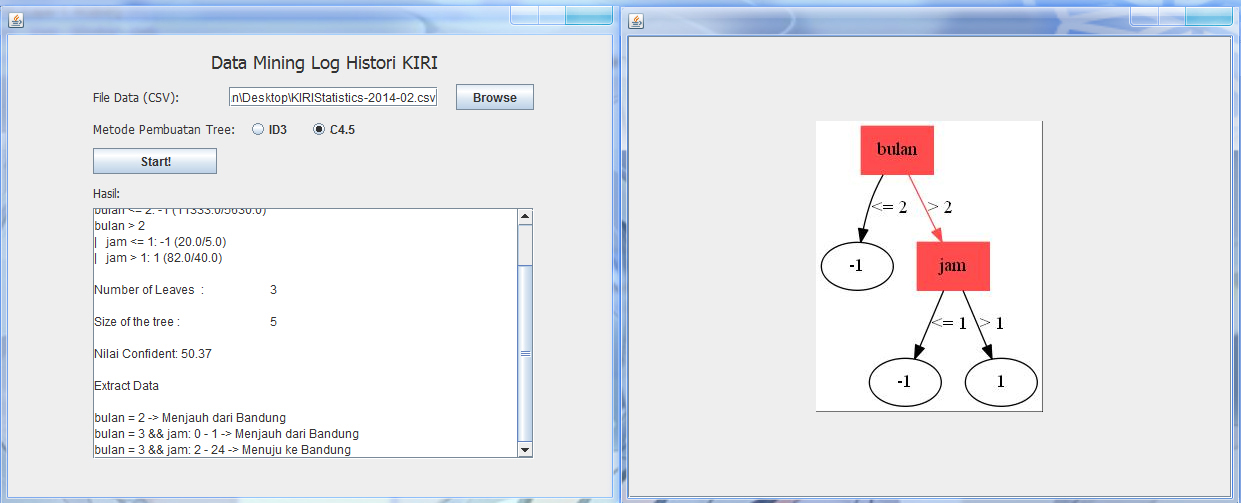
\includegraphics[scale=0.3]{Gambar/percobaan2.jpg}
\caption[Percobaan \textsl{Data Mining} dengan Menggunakan Metode C4.5 pada \textsl{Log} Histori KIRI pada Bulan 2 Tahun 2014]{Percobaan \textsl{Data Mining} dengan Menggunakan Metode C4.5 pada \textsl{Log} Histori KIRI pada Bulan 2 Tahun 2014.} 
\label{fig:percobaan2}
\end{figure}

Pada kedua percobaan, terdapat perbedaan bulan, hal ini dikarenakan perubahan waktu dari UTC menuju GMT+7 sehingga terdapat perubahan bulan atau tahun. Karena data pada bulan selanjutnya hanya tujuh jam, maka hasil pada bulan selanjutnya lebih baik tidak dianggap karena data tersebut tidak cukup untuk merepresentasikan waktu satu bulan.

Hasil percobaan pembuatan \textsl{decision tree} pada metode ID3 mengalami overfitting karena menghasilkan klasifikasi pada hampir setiap kemungkinan. Oleh karena itu, dapat disimpulkan bahwa \textsl{decision tree} dengan metode ID3 menghasilkan \textsl{tree} yang jelek. Namun pada percobaan metode C4.5, menghasilkan \textsl{decision tree} yang cukup besar namun tidak overfitting dan banyak \textsl{user} yang menjauhi Bandung. Tetapi, \textsl{tree} yang dihasilkan cukup kecil. Dapat disimpulkan hasil \textsl{decision tree} pada percobaan di bulan ini cukup jelek.

Nilai akurasi dari percobaan dengan metode ID3 adalah 38.22\% sedangkan untuk percobaan dengan metode C4.5 adalah 50.37\%, dari sini dapat dinyatakan bahwa hasil \textsl{decision tree} dari C4.5 lebih tepat daripada ID3 dan metode ID3 menghasilkan nilai akurasi yang belum memuaskan karena masih dibawah 50\%.

Selain itu, dari kedua percobaan ini, diperoleh bahwa cukup sulit untuk membaca hasil \textsl{decision tree} terutama seperti hasil \textsl{decision tree} dengan metode ID3. Oleh karena itu, ditambahkan fungsi agar \textsl{decision tree} lebih mudah dibaca. Program ditambah satu kelas baru yaitu SDForExtractData yang berfungsi untuk menyimpan data dan membuat kesimpulan dari setiap \textsl{leaf} yang dihasilkan.

%Nilai akurasi dari percobaan dengan metode ID3 adalah 37.49\% sedangkan untuk percobaan dengan metode C4.5 adalah 49.79\%, dari sini dapat dinyatakan bahwa hasil \textsl{decision tree} dari C4.5 lebih tepat daripada ID3 namun kedua metode tersebut menghasilkan nilai akurasi yang belum memuaskan, karena masih dibawah 50\%

%Selain itu, dari kedua percobaan ini, diperoleh bahwa cukup sulit untuk membaca hasil \textsl{decision tree} terutama pada \textsl{node} dengan kedalaman lebih dari 4 tingkat. Oleh karena itu, akan ditambahkan fungsi agar \textsl{decision tree} lebih mudah dibaca. Program akan ditambah satu kelas baru yaitu SDForExtractData yang berfungsi untuk menyimpan data dan membuat kesimpulan dari setiap \textsl{leaf} yang dihasilkan.

Berikut hasil dari fungsi yang dibuat agar \textsl{decision tree} lebih mudah dibaca, dapat dilihat pada gambar \ref{fig:percobaan3}. Dengan fungsi tersebut, diharapkan user dapat lebih mudah membaca \textsl{decision tree} yang dihasilkan.

\begin{figure}[H]
\centering
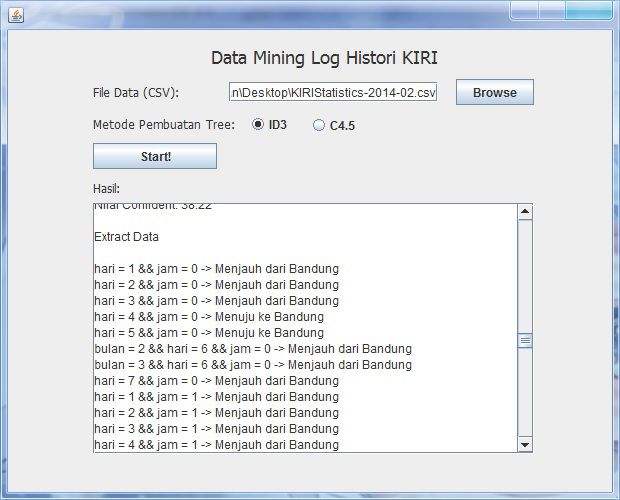
\includegraphics[scale=0.7]{Gambar/percobaan3.jpg}
\caption[Hasil dari SDForExtractData]{Hasil dari SDForExtractData} 
\label{fig:percobaan3}
\end{figure}

\subsection{Analisis Hasil Uji}

Berdasarkan pengujian di atas, dapat disimpulkan bahwa 

\begin{enumerate}
	\item Metode ID3 menghasilkan \textsl{decision tree} yang bersifat overfitting pada data \textsl{log} histori KIRI dengan  \textsl{preprocessing data} dan klasifikasi yang sudah dijelaskan pada bab 3.
	\item Metode C4.5 menghasilkan \textsl{decision tree} yang lebih baik dan tepat daripada ID3, khususnya pada data \textsl{log} histori KIRI dengan \textsl{preprocessing data} dan klasifikasi yang sudah dijelaskan pada bab 3 (C4.5 menghasilkan 50.37\% sedangkan ID3 menghasilkan 38.22\%).
	\item Metode ID3 belum menghasilkan nilai akurasi yang memuaskan, karena masih dibawah 50\%.
	\item Dari data \textsl{log} histori KIRI pada bulan Febuari 2014, \textsl{decision tree} dengan metode C4.5 menyatakan bahwa \textsl{user} lebih sering menjauhi Bandung daripada mendekati Bandung atau berangkat menuju daerah yang sama.
	\item \textsl{Decision tree} yang dihasilkan di bulan ini tidak memberikan nilai lebih yang signifikan dibandingkan statistik biasa karena \textsl{decision tree} yang dihasilkan hanya memiliki satu \textsl{leaf}.
	%\item Metode C4.5 menghasilkan \textsl{decision tree} yang lebih baik dan tepat daripada ID3, khususnya pada data \textsl{log} histori KIRI dengan \textsl{preprocessing data} dan klasifikasi yang sudah dijelaskan pada bab 3 (C4.5 menghasilkan 49.79\% sedangkan ID3 menghasilkan 37.49\%).
	%\item Kedua metode belum menghasilkan nilai akurasi yang memuaskan, karena masih dibawah 50\%.
	%\item Dari data \textsl{log} histori KIRI pada bulan Febuari 2014, \textsl{decision tree} dengan metode C4.5 menyatakan bahwa \textsl{user} sering menjauhi Bandung dan mendekati Bandung, namun hampir tidak ada \textsl{user} yang berangkat menuju daerah yang sama. Dari pernyataan tersebut, dapat disimpulkan bahwa \textsl{user} sering berpergian dengan jarak lebih dari satu kilometer.
\end{enumerate}













}{}
\ifdefstring{\vbabf}{1}{\chapter{Kesimpulan dan Saran}

\section{Kesimpulan}

Kesimpulan yang dapat diambil dari penelitian \textsl{data mining log} histori KIRI ini adalah 

Salah satu cara untuk memperoleh pola yang menarik dan bermakna, diperlukan pengolahan data dengan cara membuat klasifikasi dari data yang dihasilkan sesuai dengan tujuan yang ingin dicari. Pada penelitian ini dilakukan klasifikasi tujuan dari \textsl{user} apakah mereka ingin menuju Bandung atau keluar Bandung atau masih berada di area yang sama sehingga diperoleh pergerakan \textsl{user} KIRI di Bandung.

Pembuatan perangkat lunak untuk melakukan \textsl{data mining} pada \textsl{log} histori KIRI dapat dilakukan.

Pola yang diperoleh dari data \textsl{log} histori KIRI adalah \textsl{user} sering pergi menjauhi Bandung pada bulan Febuari 2014.

\section{Saran}
Untuk pengembangan aplikasi \textsl{data mining log} histori KIRI lebih lanjut, dapat dilakukan dengan cara menggunakan klasifikasi yang lebih baik dan detail. Perbedaannya dengan manggunakan klasifikasi yang lebih detail adalah hasil dari \textsl{decision tree} mungkin lebih besar (jika dibandingkan dengan \textsl{decision tree} yang dihasilkan dengan metode C4.5) namun diharapkan lebih memiliki makna dan dapat menghasilkan nilai akurasi yang lebih besar.

%Untuk pengembangan aplikasi \textsl{data mining log} histori KIRI lebih lanjut, dapat dilakukan dengan cara menggunakan klasifikasi yang lebih baik dan detail. Perbedaannya dengan manggunakan klasifikasi yang lebih detail adalah hasil dari \textsl{decision tree} belum tentu lebih kecil namun diharapkan lebih memiliki makna dan dapat menghasilkan nilai akurasi yang lebih besar.}{}
\ifdefstring{\vbabg}{1}{\include{Bab/bab7}}{}
\ifdefstring{\vbabh}{1}{\include{Bab/bab8}}{}
\ifdefstring{\vbabi}{1}{\include{Bab/bab9}}{}

\bibliographystyle{ieeetr}
\bibliography{pustaka}

\appendix
\apptoc

\tampillmp{\vlmp}
\begin{landscape}
\ifdefstring{\vlmpa}{1}{\include{Lampiran/lampA}}{}
\end{landscape}
\ifdefstring{\vlmpb}{1}{\chapter{The Source Code}
\label{app:B}

%selalu gunakan single spacing untuk source code !!!!!
\singlespacing 
% language: bahasa dari kode program
% terdapat beberapa pilihan : Java, C, C++, PHP, Matlab, R, dll
%
% basicstyle : ukuran font untuk kode program
% terdapat beberapa pilihan : tiny, scriptsize, footnotesize, dll
%
% caption : nama yang akan ditampilkan di dokumen akhir, lihat contoh
\begin{lstlisting}[language=Java,basicstyle=\tiny,caption=Controller.java]
package DataMiningLogHistoriKIRIWithoutDateAndMinutes;

import java.awt.image.BufferedImage;
import java.io.BufferedWriter;
import java.io.File;
import java.io.FileWriter;
import java.io.IOException;
import java.io.PrintWriter;
import java.util.ArrayList;
import javax.imageio.ImageIO;
import javax.swing.ImageIcon;
import javax.swing.JFrame;
import javax.swing.JLabel;
import javax.swing.JScrollPane;
import javax.swing.JTextArea;
import weka.core.Instances;

/**
 *
 * @author Jovan Gunawan
 */
public class Controller
{
    public Controller()
    {
    }
    
    public void startMining(String inputFilePath, String miningAlgo, JLabel label, JTextArea textArea) throws IOException
    {
        CSVReader csv = new CSVReader();
        ArrayList<String[]> data = csv.readCSV(inputFilePath);
        
        ArrayList<String[]> findRoute = new ArrayList<String[]>();
        ProcessingData pd = new ProcessingData();
        pd.processSorting(findRoute, data, "FINDROUTE");
        
        //int maxMin digunakan untuk menyimpan nilai max dan min dari variable bulan dan tahun. Untuk ketentuan posisi array dapat dilihat di method preprocessing data
        int[] maxMin = new int[4];
        ArrayList<int[]> dataAfterPreprocessing = pd.preprocessingData(findRoute, maxMin);
        
        ArffIO io = new ArffIO();
        io.writeArrf("tempArff", dataAfterPreprocessing);
        
        Instances arff = io.readArff("temp.arff");
        //arff.setClassIndex(arff.numAttributes() - 1);
        DecisionTree dt = new DecisionTree();
        String [] tempTreeDataResult;
        System.out.println(miningAlgo);
        if(miningAlgo.equals("id3"))
        {
             textArea.setText(dt.id3(arff));
        }
        else
        {
             textArea.setText(dt.j48(arff));
        }
        tempTreeDataResult = textArea.getText().split("\n");
        textArea.setText(textArea.getText() + "\nNilai Confident: " + dt.calculatePrecision(arff) + "\n");
        String[] treeDataResult;
        System.out.println(tempTreeDataResult.length);
        if(tempTreeDataResult.length < 8)
        {
            if(miningAlgo.equals("id3"))
            {
                treeDataResult = new String[tempTreeDataResult.length-2];
            }
            else
            {
                treeDataResult = new String[tempTreeDataResult.length-6];
            }
            System.arraycopy(tempTreeDataResult, 2, treeDataResult, 0, treeDataResult.length);
        }
        else
        {
            if(miningAlgo.equals("id3"))
            {
                treeDataResult = new String[tempTreeDataResult.length-3];
            }
            else
            {
                treeDataResult = new String[tempTreeDataResult.length-7];
            }
            System.arraycopy(tempTreeDataResult, 3, treeDataResult, 0, treeDataResult.length);
        }
        System.out.println(treeDataResult[0]);
        SDForConvertTree dataTree = new SDForConvertTree(treeDataResult);
        
        try {
            PrintWriter out = new PrintWriter(new BufferedWriter(new FileWriter("tree.txt")));
            SDForExtractData extract = new SDForExtractData(new String[]{"bulan", "tahun", "hari", "jam"},new int[]{maxMin[0],maxMin[1],7,24}, new int[]{maxMin[2],maxMin[3],1,0});
            out.println("digraph{" + DotConverter.convert(dataTree, extract, miningAlgo, 0, "") + "}");
            out.close();
            
            textArea.setText(textArea.getText());
            ArrayList<String> extractData = extract.getList();
            
            if(extractData.size() > 0)
            {
                textArea.setText(textArea.getText() + "\nExtract Data\n");
            }
            for(int i = 0; i < extractData.size(); i++)
            {
                textArea.setText(textArea.getText() + "\n" + extractData.get(i));
            }
            
        } catch (IOException ex) {
            System.out.println("Error ketika menulis file txt");
        }
        
        Cmd.makeJpgUsingDotCommand();
        
        JFrame jf2 = new JFrame();
        
        jf2.setVisible(true);
        jf2.setSize(620, 500);
        BufferedImage image = null;
        image = ImageIO.read(new File("tree.jpg"));
        ImageIcon image2 = new ImageIcon(image);
        JLabel labels = new JLabel(image2);
        JScrollPane pane = new JScrollPane(labels);
        jf2.setContentPane(pane);
    }
    
    
    public static void main (String [] args) 
    {
        Controller cont = new Controller();
        
        JFrame jf = new JFrame();
        View v = new View(cont);
        
        jf.setVisible(true);
        jf.setSize(620, 500);
        jf.setDefaultCloseOperation(JFrame.EXIT_ON_CLOSE);
        
        jf.add(v);
    }
}

\end{lstlisting}

\begin{lstlisting}[language=Java,basicstyle=\tiny,caption=View.java]
package DataMiningLogHistoriKIRIWithoutDateAndMinutes;

import java.io.File;
import java.io.IOException;
import java.util.logging.Level;
import java.util.logging.Logger;
import javax.swing.JFileChooser;

/**
 *
 * @author Jovan Gunawan
 */
public class View extends javax.swing.JPanel {

    /**
     * Creates new form View
     */
    public View(Controller cont) {
        this.cont = cont;
        initComponents();
        buttonGroup1.add(radioButtonId3);
        buttonGroup1.add(radioButtonC45);
    }

    /**
     * This method is called from within the constructor to initialize the form.
     * WARNING: Do NOT modify this code. The content of this method is always
     * regenerated by the Form Editor.
     */
    @SuppressWarnings("unchecked")
    // <editor-fold defaultstate="collapsed" desc="Generated Code">                          
    private void initComponents() {

        buttonGroup1 = new javax.swing.ButtonGroup();
        judul = new javax.swing.JLabel();
        labelFileData = new javax.swing.JLabel();
        labelPemilihanMethod = new javax.swing.JLabel();
        radioButtonId3 = new javax.swing.JRadioButton();
        radioButtonC45 = new javax.swing.JRadioButton();
        textFieldFilePath = new javax.swing.JTextField();
        buttonStart = new javax.swing.JButton();
        scrollPanel = new javax.swing.JScrollPane();
        hasil = new javax.swing.JTextArea();
        labelHasil = new javax.swing.JLabel();
        buttonBrowse = new javax.swing.JButton();
        labelKeterangan = new javax.swing.JLabel();

        judul.setFont(new java.awt.Font("Tahoma", 0, 18)); // NOI18N
        judul.setHorizontalAlignment(javax.swing.SwingConstants.CENTER);
        judul.setText("Data Mining Log Histori KIRI");

        labelFileData.setFont(new java.awt.Font("Tahoma", 0, 12)); // NOI18N
        labelFileData.setText("File Data (CSV):");

        labelPemilihanMethod.setFont(new java.awt.Font("Tahoma", 0, 12)); // NOI18N
        labelPemilihanMethod.setText("Metode Pembuatan Tree:");

        radioButtonId3.setSelected(true);
        radioButtonId3.setText("ID3");

        radioButtonC45.setText("C45");
        radioButtonC45.addActionListener(new java.awt.event.ActionListener() {
            public void actionPerformed(java.awt.event.ActionEvent evt) {
                radioButtonC45ActionPerformed(evt);
            }
        });

        buttonStart.setText("Start!");
        buttonStart.addActionListener(new java.awt.event.ActionListener() {
            public void actionPerformed(java.awt.event.ActionEvent evt) {
                buttonStartActionPerformed(evt);
            }
        });

        hasil.setColumns(20);
        hasil.setRows(5);
        scrollPanel.setViewportView(hasil);

        labelHasil.setFont(new java.awt.Font("Tahoma", 0, 12)); // NOI18N
        labelHasil.setText("Hasil:");

        buttonBrowse.setText("Browse");
        buttonBrowse.addActionListener(new java.awt.event.ActionListener() {
            public void actionPerformed(java.awt.event.ActionEvent evt) {
                buttonBrowseActionPerformed(evt);
            }
        });

        labelKeterangan.setFont(new java.awt.Font("Tahoma", 0, 12)); // NOI18N

        javax.swing.GroupLayout layout = new javax.swing.GroupLayout(this);
        this.setLayout(layout);
        layout.setHorizontalGroup(
            layout.createParallelGroup(javax.swing.GroupLayout.Alignment.LEADING)
            .addGroup(javax.swing.GroupLayout.Alignment.TRAILING, layout.createSequentialGroup()
                .addGroup(layout.createParallelGroup(javax.swing.GroupLayout.Alignment.TRAILING)
                    .addGroup(javax.swing.GroupLayout.Alignment.LEADING, layout.createSequentialGroup()
                        .addGap(117, 117, 117)
                        .addComponent(judul, javax.swing.GroupLayout.PREFERRED_SIZE, 399, javax.swing.GroupLayout.PREFERRED_SIZE)
                        .addGap(0, 0, Short.MAX_VALUE))
                    .addGroup(javax.swing.GroupLayout.Alignment.LEADING, layout.createSequentialGroup()
                        .addGap(85, 85, 85)
                        .addGroup(layout.createParallelGroup(javax.swing.GroupLayout.Alignment.LEADING)
                            .addGroup(layout.createSequentialGroup()
                                .addComponent(labelFileData, javax.swing.GroupLayout.DEFAULT_SIZE, 138, Short.MAX_VALUE)
                                .addPreferredGap(javax.swing.LayoutStyle.ComponentPlacement.UNRELATED)
                                .addComponent(textFieldFilePath, javax.swing.GroupLayout.PREFERRED_SIZE, 209, javax.swing.GroupLayout.PREFERRED_SIZE)
                                .addGap(18, 18, 18)
                                .addComponent(buttonBrowse))
                            .addGroup(layout.createSequentialGroup()
                                .addGroup(layout.createParallelGroup(javax.swing.GroupLayout.Alignment.LEADING, false)
                                    .addGroup(layout.createSequentialGroup()
                                        .addComponent(labelPemilihanMethod, javax.swing.GroupLayout.PREFERRED_SIZE, 147, javax.swing.GroupLayout.PREFERRED_SIZE)
                                        .addPreferredGap(javax.swing.LayoutStyle.ComponentPlacement.RELATED)
                                        .addComponent(radioButtonId3)
                                        .addGap(18, 18, 18)
                                        .addComponent(radioButtonC45))
                                    .addComponent(buttonStart, javax.swing.GroupLayout.PREFERRED_SIZE, 124, javax.swing.GroupLayout.PREFERRED_SIZE)
                                    .addComponent(labelHasil, javax.swing.GroupLayout.PREFERRED_SIZE, 89, javax.swing.GroupLayout.PREFERRED_SIZE)
                                    .addComponent(scrollPanel, javax.swing.GroupLayout.DEFAULT_SIZE, 441, Short.MAX_VALUE)
                                    .addComponent(labelKeterangan, javax.swing.GroupLayout.DEFAULT_SIZE, javax.swing.GroupLayout.DEFAULT_SIZE, Short.MAX_VALUE))
                                .addGap(0, 0, Short.MAX_VALUE)))))
                .addGap(84, 84, 84))
        );
        layout.setVerticalGroup(
            layout.createParallelGroup(javax.swing.GroupLayout.Alignment.LEADING)
            .addGroup(layout.createSequentialGroup()
                .addContainerGap()
                .addComponent(judul, javax.swing.GroupLayout.PREFERRED_SIZE, 31, javax.swing.GroupLayout.PREFERRED_SIZE)
                .addPreferredGap(javax.swing.LayoutStyle.ComponentPlacement.RELATED)
                .addGroup(layout.createParallelGroup(javax.swing.GroupLayout.Alignment.BASELINE)
                    .addComponent(labelFileData, javax.swing.GroupLayout.PREFERRED_SIZE, 26, javax.swing.GroupLayout.PREFERRED_SIZE)
                    .addComponent(textFieldFilePath, javax.swing.GroupLayout.PREFERRED_SIZE, javax.swing.GroupLayout.DEFAULT_SIZE, javax.swing.GroupLayout.PREFERRED_SIZE)
                    .addComponent(buttonBrowse))
                .addPreferredGap(javax.swing.LayoutStyle.ComponentPlacement.RELATED)
                .addGroup(layout.createParallelGroup(javax.swing.GroupLayout.Alignment.BASELINE)
                    .addComponent(labelPemilihanMethod, javax.swing.GroupLayout.PREFERRED_SIZE, 26, javax.swing.GroupLayout.PREFERRED_SIZE)
                    .addComponent(radioButtonC45)
                    .addComponent(radioButtonId3))
                .addPreferredGap(javax.swing.LayoutStyle.ComponentPlacement.RELATED)
                .addComponent(buttonStart)
                .addPreferredGap(javax.swing.LayoutStyle.ComponentPlacement.RELATED)
                .addComponent(labelHasil, javax.swing.GroupLayout.PREFERRED_SIZE, 26, javax.swing.GroupLayout.PREFERRED_SIZE)
                .addGap(2, 2, 2)
                .addComponent(scrollPanel, javax.swing.GroupLayout.PREFERRED_SIZE, 251, javax.swing.GroupLayout.PREFERRED_SIZE)
                .addPreferredGap(javax.swing.LayoutStyle.ComponentPlacement.RELATED, 10, Short.MAX_VALUE)
                .addComponent(labelKeterangan, javax.swing.GroupLayout.PREFERRED_SIZE, 26, javax.swing.GroupLayout.PREFERRED_SIZE))
        );
    }// </editor-fold>                        

    private void buttonBrowseActionPerformed(java.awt.event.ActionEvent evt) {                                             
        final JFileChooser fc = new JFileChooser();
        int returnVal = fc.showOpenDialog(buttonStart);

        if (returnVal == JFileChooser.APPROVE_OPTION) {
            File file = fc.getSelectedFile();
            textFieldFilePath.setText(file.getPath());
        } else {
            System.out.println("Error in capture the path");
            System.exit(1);
        }
    }                                            

    private void buttonStartActionPerformed(java.awt.event.ActionEvent evt) {                                            
        String inputPath = textFieldFilePath.getText();
        String miningAlgo = "";
        if(radioButtonId3.isSelected())
        {
            miningAlgo = "id3";
        }
        else
        {
            miningAlgo = "c45";
        }
        
        try {
            cont.startMining(inputPath, miningAlgo, labelKeterangan, hasil);
        }catch(IOException e)
        {
            System.out.println("Error start mining");
            System.exit(1);
        }
    }                                           

    private void radioButtonC45ActionPerformed(java.awt.event.ActionEvent evt) {                                               
        // TODO add your handling code here:
    }                                              


    // Variables declaration - do not modify                     
    private javax.swing.JButton buttonBrowse;
    private javax.swing.ButtonGroup buttonGroup1;
    private javax.swing.JButton buttonStart;
    private javax.swing.JTextArea hasil;
    private javax.swing.JLabel judul;
    private javax.swing.JLabel labelFileData;
    private javax.swing.JLabel labelHasil;
    private javax.swing.JLabel labelKeterangan;
    private javax.swing.JLabel labelPemilihanMethod;
    private javax.swing.JRadioButton radioButtonId3;
    private javax.swing.JRadioButton radioButtonC45;
    private javax.swing.JScrollPane scrollPanel;
    private javax.swing.JTextField textFieldFilePath;
    // End of variables declaration                   
    private Controller cont;
}

\end{lstlisting}

\begin{lstlisting}[language=Java,basicstyle=\tiny,caption=CSVReader.java]
package DataMiningLogHistoriKIRIWithoutDateAndMinutes;

import java.io.BufferedReader;
import java.io.FileReader;
import java.io.IOException;
import java.util.ArrayList;
import java.util.Set;

/**
 *
 * @author Jovan Gunawan
 */
public class CSVReader
{
    private ArrayList<String[]> data;
    private int banyakAtribut;
    public CSVReader() 
    {
        data = new ArrayList<String[]>();
        banyakAtribut = 0;
    }

    public void setEmpty()
    {
        getData().clear();
    }
    public ArrayList readCSV(String [] file)
    {
        for(int i = 0; i < file.length; i++)
        {
            readCSV(file[i]);
        }
        return getData();
    }
    public ArrayList readCSV(String file)
    {
        try
        {
            String temp;
            String [] splited;
            int i=0;
            BufferedReader br = new BufferedReader(new FileReader(file));
            while ((temp = br.readLine()) != null)
            {
                splited = temp.split("\"");
                if(i==0)
                {
                    //baca atributnya terlebih dahulu
                    ArrayList al = new ArrayList<String>();
                    String tempAtribut ="";
                    for(int j = 0; j < splited.length; j++)
                    {
                        if(j%2 == 0)
                        {
                            String [] splitedKoma = splited[j].split(",");
                            for(int k = 0; k < splitedKoma.length; k++)
                            {
                                if(!(k == 0 && splitedKoma[k].length() ==0)||(k==splitedKoma.length-1 && splitedKoma[k].length() == 0))
                                {
                                    al.add(splitedKoma[k]);
                                }
                            }
                        }
                        else
                        {
                            al.add(splited[j]);
                        }
                    }
                    banyakAtribut = al.size();
                    String[] tempDataAtribut = new String[banyakAtribut];
                    for(int j = 0; j < banyakAtribut; j++)
                    {
                        tempDataAtribut[j] = (String)al.get(j);
                    }
                    getData().add(tempDataAtribut);
                    i++;
                }
                else
                {
                    //baca untuk datanya
                    int index = 0;
                    String [] tempData = new String[banyakAtribut];
                    for(int j = 0; j < splited.length; j++)
                    {
                        if(j%2 == 0)
                        {
                            String [] splitedKoma = splited[j].split(",");
                            for(int k = 0; k < splitedKoma.length; k++)
                            {
                                if(!(k == 0 && splitedKoma[k].length() ==0)||(k==splitedKoma.length-1 && splitedKoma[k].length() == 0))
                                {
                                    tempData[index] = splitedKoma[k];
                                    index++;
                                }
                            }
                        }
                        else
                        {
                            tempData[index] = splited[j];
                            index++;
                        }
                    }
                    getData().add(tempData);
                    i++;
                }
            }
            for(int j = 0; j < i; j++)
            {
                String [] temp2 = (String[])getData().get(j);
            }
            br.close();
        }catch(IOException e)
        {
            System.out.println("Failed to read data");
        }
        return getData();
    }

    public ArrayList getData()
    {
        return data;
    }
    public void setData(ArrayList data)
    {
        this.data = data;
    }
    public int getBanyakAtribut()
    {
        return banyakAtribut;
    }
    public void setBanyakAtribut(int banyakAtribut)
    {
        this.banyakAtribut = banyakAtribut;
    }
}
\end{lstlisting}

\begin{lstlisting}[language=Java,basicstyle=\tiny,caption=ProcessingData.java]
package DataMiningLogHistoriKIRIWithoutDateAndMinutes;

import java.util.ArrayList;

/**
 *
 * @author Jovan Gunawan
 */
public class ProcessingData
{
    ProcessingData()
    {
    }

    public void processSorting(ArrayList addApiKey, ArrayList findRoute, ArrayList login, ArrayList nearbyTransport, ArrayList pageLoad, ArrayList register, ArrayList searchPlace, ArrayList widgetError, ArrayList widgetLoad, ArrayList data)
    {
        System.out.println("Banyak Data: " + data.size());
        for(int i =0; i < data.size(); i++)
        {
            String [] tempData = (String[])data.get(i);
            if(tempData[3].equals("ADDAPIKEY"))
            {
                addApiKey.add(tempData);
            }
            else if(tempData[3].equals("FINDROUTE"))
            {
                findRoute.add(tempData);
            }
            else if(tempData[3].equals("LOGIN"))
            {
                login.add(tempData);
            }
            else if(tempData[3].equals("NEARBYTRANSPORT"))
            {
                nearbyTransport.add(tempData);
            }
            else if(tempData[3].equals("PAGELOAD"))
            {
                pageLoad.add(tempData);
            }
            else if(tempData[3].equals("REGISTER"))
            {
                register.add(tempData);
            }
            else if(tempData[3].equals("SEARCHPLACE"))
            {
                searchPlace.add(tempData);
            }
            else if(tempData[3].equals("WIDGETERROR"))
            {
                widgetError.add(tempData);
            }
            else if(tempData[3].equals("WIDGETLOAD"))
            {
                widgetLoad.add(tempData);
            }
        }
    }
    public void processSorting(ArrayList array, ArrayList data, String action)
    {
        for(int i =0; i < data.size(); i++)
        {
            String [] tempData = (String[])data.get(i);
            if(tempData[3].equals(action))
            {
                array.add(tempData);
            }
        }
    }
    public ArrayList preprocessingData(ArrayList<String[]> data, int[] maxMin)
    {
        // 2 int[] untuk mendapatkan nilai max dan min dari varible bulan dan tahun yang digunakan untuk inisialisasi max min pada kelas SDForExtractData.
        // array pertama untuk bulan, dan array kedua untuk tahun
        int []max = new int[2];
        int []min = new int[2];
        max[0] = 0;
        max[1] = 0;
        min[0] = Integer.MAX_VALUE;
        min[1] = Integer.MAX_VALUE;
        
        ArrayList<int[]> result = new ArrayList<int[]>();
        
        // tahap pertama: ubah waktu dari UTC ke GMT+7
        for(int i = 0; i < data.size(); i++)
        {
            data.get(i)[2] = TimezoneConverter.convertToGMT7(data.get(i)[2]);
        }
        
        // tahap kedua sampai kesembilan
        DistanceHaversine haversine = new DistanceHaversine();
        for(int i = 0; i < data.size(); i++)
        {
            //cek apakah format sudah benar atau belum
            if(data.get(i)[4].split(",").length == 3)
            {
                // tahap kedua: pecah string atribut tanggal
                int[] temp = new int[5];
                String[] splited = data.get(i)[2].split(" ");
                temp[2] = Integer.parseInt(splited[0]);
                // tahap ketiga: pecah nilai string yang tanggal
                String[] splited2 = splited[1].split("/");
                temp[0] = Integer.parseInt(splited2[0]);
                temp[1] = Integer.parseInt(splited2[2]);
                // tahap keempat: pecah nilai string yang jam
                splited2 = splited[2].split(":");
                temp[3] = Integer.parseInt(splited2[0]);
                // tahap kelima: pecah string atribut additional data
                splited = data.get(i)[4].split("/");
                // tahap keenam: pecah lokasi keberangkatan dan lokasi tujuan untuk mendapatkan lat n lon dan (ini tahap ketujuh) menghitung jarak terhadap titik pusat
                splited2 = splited[0].split(",");
                double jarakKeberangkatan = haversine.calculateDistance(Double.parseDouble(splited2[0]), Double.parseDouble(splited2[1]), -6.916667,107.6) * 1000;
                splited2 = splited[1].split(",");
                double jarakTujuan = haversine.calculateDistance(Double.parseDouble(splited2[0]), Double.parseDouble(splited2[1]), -6.916667,107.6) * 1000;
                // tahap kedelapan, set semua data ke array
                temp[4] = klasifikasiKelas(jarakKeberangkatan, jarakTujuan);

                if(temp[4] != -2)
                {
                    result.add(temp);
                    //proses untuk mencatat nilai max dan min
                    if(max[0] < temp[0])
                    {
                        max[0] = temp[0];
                    }
                    if(min[0] > temp[0])
                    {
                        min[0] = temp[0];
                    }
                    if(max[1] < temp[1])
                    {
                        max[1] = temp[1];
                    }
                    if(min[1] > temp[1])
                    {
                        min[1] = temp[1];
                    }
                }
            }
            else
            {
                System.out.println("ERROR: additional data tidak sesuai; " + data.get(i)[4]);
            }
        }
        maxMin[0] = max[0];
        maxMin[1] = max[1];
        maxMin[2] = min[0];
        maxMin[3] = min[1];
        return result;
    }
    
    public int klasifikasiKelas(double jarakKeberangkatan, double jarakTujuan)
    {
        int regionKeberangkatan, regionTujuan;
        int klasifikasi = 0; // -1 --> tidak menuju Bandung, 0 --> menuju Bandung, 1 --> menuju region yang sama
        
        regionKeberangkatan = (int)jarakKeberangkatan;
        regionTujuan = (int)jarakTujuan;
        
        if(regionKeberangkatan >= 11 && regionTujuan >= 11)
        {
            return -2;
        }
        else
        {
            if (regionKeberangkatan > regionTujuan)
            {
                klasifikasi = -1;
            }
            else if (regionKeberangkatan < regionTujuan)
            {
                klasifikasi = 1;
            }
            else
            {
                klasifikasi = 0;
            }
            return klasifikasi;
        }
    }
}
\end{lstlisting}

\begin{lstlisting}[language=Java,basicstyle=\tiny,caption=TimezoneConverter.java]
package DataMiningLogHistoriKIRIWithoutDateAndMinutes;

import java.text.ParseException;
import java.text.SimpleDateFormat;
import java.util.Date;
import java.util.TimeZone;
import java.util.logging.Level;
import java.util.logging.Logger;

/**
 *
 * @author Jovan Gunawan
 */
public class TimezoneConverter 
{
    // Mengubah input waktu menjadi waktu GMT+7
    // Jika ingin mengubah dari UTC ke GMT+7 maka komputer harus set timezone ke UTC
    // input parameter string harus dalam format dd-MM-yyyy HH:mm:ss --> contoh 1/1/2014  3:51:15 AM
    // output akan mengubah waktu menjadi GMT+7 dalam String dengan format EEE MM/dd/yyyy HH:mm:ss --> contoh Wed 01/01/2014 03:51:15
    public static String convertToGMT7(String date)
    {
        Date d = null;
        long milliseconds = 0;
        
        try {
            SimpleDateFormat f = new SimpleDateFormat("MM/dd/yyyy HH:mm");
            d = (Date)f.parse(date);
        } catch (ParseException ex) {
            SimpleDateFormat f = new SimpleDateFormat("yyyy-MM-dd HH:mm:ss");
            try {
                d = (Date)f.parse(date);
            } catch (ParseException ex1) {
                Logger.getLogger(TimezoneConverter.class.getName()).log(Level.SEVERE, null, ex);
                System.exit(1);
            }
        }
        milliseconds = d.getTime();
        
        Date currentTime = new Date(milliseconds);
        // untuk hari --> 1 = senin,..., 7 = minggu
        SimpleDateFormat sdf = new SimpleDateFormat("u MM/dd/yyyy HH:mm:ss");
        
        sdf.setTimeZone(TimeZone.getTimeZone("GMT+7"));
        return sdf.format(currentTime);
    }
}
\end{lstlisting}

\begin{lstlisting}[language=Java,basicstyle=\tiny,caption=DistanceHaversine.java]
package DataMiningLogHistoriKIRIWithoutDateAndMinutes;

/**
 *
 * @author Jovan Gunawan
 */
public class DistanceHaversine
{
    private double r;
    public DistanceHaversine()
    {
         r = 6.371;
    }

    public double calculateDistance(double latitude1, double longitude1, double latitude2, double longitude2)
    {
        latitude1 = Math.toRadians(latitude1);
        longitude1 = Math.toRadians(longitude1);
        latitude2 = Math.toRadians(latitude2);
        longitude2 = Math.toRadians(longitude2);

        double dlon = longitude2 - longitude1;
        double dlat = latitude2 - latitude1;

        double a = Math.pow((Math.sin(dlat/2)),2) + Math.cos(latitude1) * Math.cos(latitude2) * Math.pow(Math.sin(dlon/2),2);

        double c = 2 * Math.atan2(Math.sqrt(a), Math.sqrt(1-a));
        return r * c;
    }
}
\end{lstlisting}

\begin{lstlisting}[language=Java,basicstyle=\tiny,caption=ArffIO.java]
package DataMiningLogHistoriKIRIWithoutDateAndMinutes;

import java.io.BufferedReader;
import java.io.BufferedWriter;
import java.io.FileReader;
import java.io.FileWriter;
import java.io.IOException;
import java.io.PrintWriter;
import java.util.ArrayList;
import java.util.logging.Level;
import java.util.logging.Logger;
import weka.core.Instances;

/**
 *
 * @author Jovan Gunawan
 */
public class ArffIO 
{
    public ArffIO()
    {
    }
    
    // method writer ini dibuat KHUSUS untuk skripsi data log KIRI
    // input berupa arraylist dengan objek int[]
    // Setiap array int, terdapat 7 nilai yaitu tanggal, bulan, tahun, hari, jam, menit, menujuBandung
    // disini nilai hari akan diubah menjadi string, 1 akan menjadi senin, ..., dan 7 akan menjadi minggu
    public void writeArrf(String name, ArrayList<int[]> data)
    {
        String result = "@relation " + name + "\n\n@attribute bulan REAL\n@attribute tahun REAL\n"
                + "@attribute hari REAL"
                + "\n@attribute jam REAL\n@attribute menujuBandung {-1,0,1}\n\n@data";
        
        for(int i = 0; i < data.size(); i++)
        {
            int[] temp = data.get(i);
            result += "\n" + temp[0] + "," + temp[1] + "," + temp[2] + "," + temp[3] + "," + temp[4]; 
        }
        
        try {
            PrintWriter out = new PrintWriter(new BufferedWriter(new FileWriter("temp.arff")));
            out.println(result);
            out.close();
        } catch (IOException ex) {
            System.out.println("Error ketika menulis file arff");
        }
    }
    
    public Instances readArff(String name) throws IOException
    {
        Instances data;
        data = new Instances(new BufferedReader(new FileReader("temp.arff")));
        data.setClassIndex(data.numAttributes() - 1);
        return data;
    }
}
\end{lstlisting}

\begin{lstlisting}[language=Java,basicstyle=\tiny,caption=DecisionTree.java]
package DataMiningLogHistoriKIRIWithoutDateAndMinutes;

import java.util.logging.Level;
import java.util.logging.Logger;
import weka.classifiers.Classifier;
import weka.classifiers.trees.Id3;
import weka.classifiers.trees.J48;
import weka.core.Instances;
import weka.filters.Filter;
import weka.filters.unsupervised.attribute.NumericToNominal;

/**
 *
 * @author Jovan Gunawan
 */
public class DecisionTree 
{
    private Classifier tree;
    
    public double calculatePrecision(Instances arff)
    {
        int nilaiBenar = 0, resultInt;
        float result = 0;
        for (int i = 0; i < arff.numInstances(); i++)
        {    
            try {
                result = (float)tree.classifyInstance(arff.instance(i));
                resultInt = Math.round(result)-1;
                if(resultInt == Integer.parseInt(arff.instance(i).stringValue(4)))
                {
                    nilaiBenar++;
                }
            } catch (Exception ex) {
            }
        }
        double confident = Math.round(nilaiBenar * 1.0 / arff.numInstances() * 10000)/100.0;
        return confident;
    }
    
    public String id3(Instances arff)
    {
        tree = new Id3();
        try {
            NumericToNominal convert= new NumericToNominal();
            String[] options= new String[2];
            options[0]="-R";
            options[1]="1-4"; 

            convert.setOptions(options);
            convert.setInputFormat(arff);

            Instances newData=Filter.useFilter(arff, convert);
            
            tree.buildClassifier(newData);
        } catch (Exception ex) {
            Logger.getLogger(Controller.class.getName()).log(Level.SEVERE, null, ex);
        }
        
        return tree.toString();
    }
    
    public String j48(Instances arff)
    {
        tree = new J48();
        try {
            tree.buildClassifier(arff);
        } catch (Exception ex) {
            Logger.getLogger(Controller.class.getName()).log(Level.SEVERE, null, ex);
        }
        
        return tree.toString();
    }
}
\end{lstlisting}

\begin{lstlisting}[language=Java,basicstyle=\tiny,caption=DotConverter.java]
package DataMiningLogHistoriKIRIWithoutDateAndMinutes;

import DataMiningLogHistoriKIRI.*;

/**
 *
 * @author Jovan Gunawan
 */
public class DotConverter 
{
    // converter dot khusus untuk skripsi data mining log histori KIRI --> output berupa tree dalam string dari weka
    public static String convert(SDForConvertTree data, SDForExtractData extract, String miningAlgo, int deep, String nodeName)
    {
        String result = "";
        String [] temp;
        String nodeName1="", nodeName2="";
        //color 1  selalu 1.0 karena merah
        double color; 
        if(deep == 0 && data.getData().length == 1 && data.getData()[0].charAt(0) == ':')
        {
            result = data.getData()[0].split(" ")[1];
        }
        else
        {
            if(miningAlgo.equals("id3"))
            {
                boolean hasNext = true;
                int loop = 0;
                while(hasNext)
                {
                    hasNext = false;

                    temp = data.getData(0).split("  ");
                    boolean iniName1 = false;

                    System.out.println("Deep: " + deep + data.getData(0));
                    temp = temp[deep].split(" ");

                    color = 0.7 - deep * 0.02;
                    if(color < 0.3)
                    {
                        color = 0.3;
                    }

                    if(nodeName.equals(""))
                    {
                        if(loop == 0)
                        {
                            nodeName1 = data.getDataNumber(temp[0]);
                        }
                        result += nodeName1 + " -> ";
                        iniName1 = true;
                    }
                    else
                    {
                        result += nodeName + " -> ";
                    }

                    SDForExtractData tempExtract = new SDForExtractData(extract);

                    if(temp[2].charAt(temp[2].length()-1) == ':')
                    {
                        // masukin data buat extract
                        tempExtract.setRules(temp[0], temp[1], Integer.parseInt(temp[2].substring(0, temp[2].length()-1)));
                        try
                        {
                            tempExtract.setKelas(Integer.parseInt(temp[3]));
                        }catch(Exception a)
                        {
                            if(temp[3] == null)
                            {
                                tempExtract.setKelas(-2);
                            }
                        }
                        tempExtract.extract();
                        extract.addStringResult(tempExtract.getList());
                        // menghasilkan daun

                        nodeName2 = data.getDataNumber(temp[3]);
                        result += nodeName2 + " [label=\"" + temp[1] + " " + temp[2].substring(0, temp[2].length()-1) +  "\"]\n";
                        if(iniName1 && loop == 0)
                        {
                            result += nodeName1 + " [label=\"" + temp[0] + "\",shape=box,style=filled,color=\"1.0 " + color + " 1.0\"]\n";
                        }
                        result += nodeName2 + " [label=\"" + temp[3] + "\"]\n";
                        data.buangArrayPertama();
                    }
                    else
                    {
                        // masukin data bwt extract
                        tempExtract.setRules(temp[0], temp[1], Integer.parseInt(temp[2]));

                        // menghasilkan node
                        String [] temp2;
                        temp2 = data.getData(1).split("  ");
                        temp2 = temp2[deep+1].split(" ");
                        nodeName2 = data.getDataNumber(temp2[0]);
                        result += nodeName2 + " [label=\"" + temp[1] + " " + temp[2] +  "\",shape=box,style=filled,color=\"1.0 " + color + " 1.0\"]\n";
                        data.buangArrayPertama();

                        SDForExtractData newExtract = new SDForExtractData(tempExtract);
                        result += DotConverter.convert(data, newExtract, miningAlgo, deep+1, nodeName2);

                        if(iniName1 && loop == 0)
                        {
                            result += nodeName1 + " [label=\"" + temp[0] + "\",shape=box,style=filled,color=\"1.0 " + color + " 1.0\"]\n";
                        }
                        result += nodeName2 + " [label=\"" + temp2[0] + "\",shape=box,style=filled,color=\"1.0 " + color + " 1.0\"]\n";
                        extract.addStringResult(newExtract.getList());
                    }
                    if(data.hasNext())
                    {
                        if(data.getData(0).split("  ").length-1 == deep)
                        {
                            hasNext = true;
                        }
                    }
                    loop++;
                }
            }
            else
            {
                for(int i = 0; i < 2; i++)
                {
                    temp = data.getData(0).split("   ");
                    boolean iniName1 = false;

                    System.out.println("Deep: " + deep + data.getData(0));
                    temp = temp[deep].split(" ");

                    color = 0.7 - deep * 0.02;
                    if(color < 0.3)
                    {
                        color = 0.3;
                    }

                    if(nodeName.equals(""))
                    {
                        if(i == 0)
                        {
                            nodeName1 = data.getDataNumber(temp[0]);
                        }
                        result += nodeName1 + " -> ";
                        iniName1 = true;
                    }
                    else
                    {
                        result += nodeName + " -> ";
                    }

                    SDForExtractData tempExtract = new SDForExtractData(extract);

                    if(temp[2].charAt(temp[2].length()-1) == ':')
                    {   
                        // masukin data bwt extract
                        tempExtract.setRules(temp[0], temp[1], Integer.parseInt(temp[2].substring(0, temp[2].length()-1)));
                        tempExtract.setKelas(Integer.parseInt(temp[3]));
                        tempExtract.extract();
                        extract.addStringResult(tempExtract.getList());
                        // menghasilkan daun
                        nodeName2 = data.getDataNumber(temp[3]);
                        result += nodeName2 + " [label=\"" + temp[1] + " " + temp[2].substring(0, temp[2].length()-1) +  "\"]\n";
                        if(iniName1 && i == 0)
                        {
                            result += nodeName1 + " [label=\"" + temp[0] + "\",shape=box,style=filled,color=\"1.0 " + color + " 1.0\"]\n";
                        }
                        result += nodeName2 + " [label=\"" + temp[3] + "\"]\n";
                        data.buangArrayPertama();
                    }
                    else 
                    {
                        // masukin data bwt extract
                        tempExtract.setRules(temp[0], temp[1], Integer.parseInt(temp[2]));
                        // menghasilkan node
                        String [] temp2;
                        temp2 = data.getData(1).split("   ");
                        temp2 = temp2[deep+1].split(" ");
                        nodeName2 = data.getDataNumber(temp2[0]);
                        result += nodeName2 + " [label=\"" + temp[1] + " " + temp[2] +  "\",shape=box,style=filled,color=\"1.0 " + color + " 1.0\"]\n";
                        data.buangArrayPertama();

                        SDForExtractData newExtract = new SDForExtractData(tempExtract);
                        result += DotConverter.convert(data, newExtract, miningAlgo, deep+1, nodeName2);

                        if(iniName1 && i == 0)
                        {
                            result += nodeName1 + " [label=\"" + temp[0] + "\",shape=box,style=filled,color=\"1.0 " + color + " 1.0\"]\n";
                        }
                        result += nodeName2 + " [label=\"" + temp2[0] + "\",shape=box,style=filled,color=\"1.0 " + color + " 1.0\"]\n";
                        extract.addStringResult(newExtract.getList());
                    }
                }
            }
        }
        return result;
    }
}
\end{lstlisting}

\begin{lstlisting}[language=Java,basicstyle=\tiny,caption=SDForConvertTree.java]
package DataMiningLogHistoriKIRIWithoutDateAndMinutes;

/**
 *
 * @author Jovan Gunawan
 * Class ini dibuat untuk struktur data yang digunakan untuk mengubah hasil output dari weka menjadi gambar dengan bahasa DOT
 * Class ini khusus untuk skripsi data mining log histori KIRI 
 * 
 * count akan digunakan untuk inisialisasi nomor data --> contoh tanggal1, tanggal 2, .... etc, angka tersebut yang akan ditaruh pada array tersebut
 * array count akan digunakan sebagai berikut --> [0] = tanggal, [1] = bulan, [2] = tahun, [3] = hari, [4] = jam, [5] = menit, [6] = nilai 0, [7] = nilai 1 , [8] = nilai 2
 */
public class SDForConvertTree 
{
    private String[] data;
    private int [] count;
    
    public SDForConvertTree(String [] data)
    {
        this.data = data;
        count = new int[9];
        for(int i = 0; i < 9; i++)
        {
            count[i] = 0;
        }
    }
    
    public void setData(String data, int index)
    {
        this.data[index] = data;
    }
    public String[] getData()
    {
        return data;
    }
    public String getData(int index)
    {
        return this.data[index];
    }
    public void setCount(int count, int index)
    {
        this.count[index] = count;
    }
    public int getCount(int index)
    {
        int temp = this.count[index];
        this.count[index]++;
        return temp;
    }
    public boolean hasNext()
    {
        if(this.data.length > 0)
        {
            return true;
        }
        else
        {
            return false;
        }
    }
    
    public void buangArrayPertama()
    {
        String[] temp = new String [data.length-1];
        System.arraycopy(data, 1, temp, 0, data.length-1);
        data = temp;
    }
    public String getDataNumber(String atribut)
    {
        String result = atribut;
        if(atribut.equals("tanggal"))
        {
            result += count[0];
            count[0]++;
        }
        else if(atribut.equals("bulan"))
        {
            result += count[1];
            count[1]++;
        }
        else if(atribut.equals("tahun"))
        {
            result += count[2];
            count[2]++;
        }
        else if(atribut.equals("hari"))
        {
            result += count[3];
            count[3]++;
        }
        else if(atribut.equals("jam"))
        {
            result += count[4];
            count[4]++;
        }
        else if(atribut.equals("menit"))
        {
            result += count[5];
            count[5]++;
        }
        else if(atribut.equals("-1"))
        {
            result += count[6];
            count[6]++;
        }
        else if(atribut.equals("1"))
        {
            result += count[7];
            count[7]++;
        }
        else if(atribut.equals("0"))
        {
            result += count[8];
            count[8]++;
        }
        return result;
    }
}
\end{lstlisting}

\begin{lstlisting}[language=Java,basicstyle=\tiny,caption=SDForExtractData.java]
package DataMiningLogHistoriKIRIWithoutDateAndMinutes;

import java.util.ArrayList;

/**
 *
 * @author Jovan Gunawan
 */
public class SDForExtractData 
{
    private String[] atribut;
    private boolean[] check;
    private int[] batasAtas;
    private int[] batasBawah;
    private int[] maxBatasAtas;
    private int[] minBatasBawah;
    private int kelas;
    private ArrayList<String> list;
    
    public SDForExtractData(String[] atribut, int[] max, int[] min)
    {
        int length = atribut.length;
        this.atribut = new String[length];
        this.maxBatasAtas = new int[length];
        this.minBatasBawah = new int[length];
        this.batasAtas = new int[length];
        this.batasBawah = new int[length];
        this.check = new boolean[length];
        list = new ArrayList<String>();
        
        for(int i = 0; i < length; i++)
        {
            this.atribut[i] = atribut[i];
            this.maxBatasAtas[i] = max[i];
            this.batasAtas[i] = max[i];
            this.minBatasBawah[i] = min[i];
            this.batasBawah[i] = min[i];
            check[i] = false;
        }
    }
    
    public SDForExtractData(SDForExtractData data)
    {
        String[] atribut = data.getAtribut();
        int[] max = data.getMaxBatasAtas();
        int[] min = data.getMinBatasBawah();
        int[] bmax = data.getBatasAtas();
        int[] bmin = data.getBatasBawah();
        boolean[] check = data.getCheck();
        int length = data.getAtribut().length;
        list = data.getList();
        
        this.atribut = new String[length];
        this.maxBatasAtas = new int[length];
        this.minBatasBawah = new int[length];
        this.batasAtas = new int[length];
        this.batasBawah = new int[length];
        this.check = new boolean[length];
        
        for(int i = 0; i < length; i++)
        {
            this.atribut[i] = atribut[i];
            this.maxBatasAtas[i] = max[i];
            this.batasAtas[i] = bmax[i];
            this.minBatasBawah[i] = min[i];
            this.batasBawah[i] = bmin[i];
            this.check[i] = check[i];
        }
    }
    
    public void setKelas(int kelas)
    {
        this.kelas = kelas;
    }
    
    public void setRules(String atribut, String rulesOperation, int value)
    {
        int index = 0;
        for(int i = 0; i < this.atribut.length; i++)
        {
            if(this.atribut[i].equals(atribut))
            {
                index = i;
                break;
            }
        }
        check[index] = true;
        
        if(rulesOperation.equals("<="))
        {
            batasAtas[index] = value;
        }
        else if(rulesOperation.equals("<"))
        {
            batasAtas[index] = value-1;
        }
        else if(rulesOperation.equals(">="))
        {
            batasBawah[index] = value;
        }
        else if(rulesOperation.equals(">"))
        {
            batasBawah[index] = value+1;
        }
        else if(rulesOperation.equals("="))
        {
            batasAtas[index] = value;
            batasBawah[index] = value;
        }
    }
    
    public void extract()
    {
        String[] hari = new String[]{"Senin", "Selasa", "Rabu", "Kamis", "Jumat", "Sabtu", "Minggu"};
        boolean in = false;
        String result = "";
        for(int i = 0; i < atribut.length; i++)
        {
            if(check[i])
            {
                if(in)
                {
                    result += " && ";
                }
                if(batasBawah[i] == batasAtas[i])
                {
                    result += atribut[i] + " = " + batasAtas[i];
                }
                else
                {
                    result += atribut[i] + ": " + batasBawah[i] + " - " + batasAtas[i]; 
                }
                in = true;
            }
        }
        
        if(kelas == 1)
        {
            result += " -> Menuju ke Bandung";
        }
        else if(kelas == 0)
        {
            result += " -> Menuju daerah yang sama";
        }
        else
        {
            result += " -> Menjauh dari Bandung";
        }
        list.add(result);
    }
    
    public void addStringResult(ArrayList<String> result)
    {
        list = result;
    }

    public String[] getAtribut() {
        return atribut;
    }

    public boolean[] getCheck() {
        return check;
    }

    public int[] getBatasAtas() {
        return batasAtas;
    }

    public int[] getBatasBawah() {
        return batasBawah;
    }

    public int[] getMaxBatasAtas() {
        return maxBatasAtas;
    }

    public int[] getMinBatasBawah() {
        return minBatasBawah;
    }

    public int getKelas() {
        return kelas;
    }

    public ArrayList<String> getList() {
        return list;
    }
    
}
\end{lstlisting}

\begin{lstlisting}[language=Java,basicstyle=\tiny,caption=CMD.java]
package DataMiningLogHistoriKIRIWithoutDateAndMinutes;

import java.io.BufferedReader;
import java.io.IOException;
import java.io.InputStreamReader;

/**
 *
 * @author Jovan Gunawan
 */
public class Cmd 
{
    public static void makeJpgUsingDotCommand()
    {
        try {
            final String dir = System.getProperty("user.dir");
            
            ProcessBuilder builder = new ProcessBuilder(
            "cmd.exe", "/c", "cd graphviz && cd bin && dot \"" + dir + "\\tree.txt\" -o \"" + dir + "\\tree.jpg\" -Tjpg ");
            builder.redirectErrorStream(true);
            Process p = builder.start();
            BufferedReader r = new BufferedReader(new InputStreamReader(p.getInputStream()));
            String line;
            while (true) {
                line = r.readLine();
                if (line == null) 
                { 
                    break; 
                }
                System.out.println(line);
            }
        } catch (IOException e) {
            System.out.println("Error ketika proses CMD");
            System.exit(1);
        }
    }
}
\end{lstlisting}}{}
%\ifdefstring{\vlmpc}{1}{\include{Lampiran/lampC}}{}
%\ifdefstring{\vlmpd}{1}{\include{Lampiran/lampD}}{}
%\ifdefstring{\vlmpe}{1}{\include{Lampiran/lampE}}{}
%\ifdefstring{\vlmpf}{1}{\include{Lampiran/lampF}}{}
%\ifdefstring{\vlmpg}{1}{\include{Lampiran/lampG}}{}
%\ifdefstring{\vlmph}{1}{\include{Lampiran/lampH}}{}
%\ifdefstring{\vlmpi}{1}{\include{Lampiran/lampI}}{}

\end{document}
